
\graphicspath{{part_2/figures}{part_2/figures/}}




% 
% \section{Euler's method applied to control synthesis}\label{sec:background}
% In this Section, we recall the results obtained in \cite{SNR17}.
% We first give results concerning a system governed by a single ODE system
% (Section \ref{ss:ODE}), then consider results for a switched system composed
% of several ODEs (Section \ref{ss:switch}).
% \subsection{ODE systems}\label{ss:ODE}
% We make the following hypothesis:
% %
% $$(H0)\quad
% %\mbox{ For all  $j\in U$,
% \mbox{ $f$ is a locally Lipschitz continuous map}.$$
% 
% %As in \cite{girard2010approximately},
% We make the assumption that the vector field $f$ is such that the
% solutions of the differential equation  (\ref{eq:sys_part4}) are defined. %, e.g. by assuming that the support of the vector field $f$ is compact.
% We will denote by $\phi(t; x^0)$ the
% solution at time~$t$ of the system:
% 
% \begin{equation}
% \begin{aligned}
%   \dot  x(t) & =  f( x(t)), \\
%    x(0) & =   x^0. \\
% %  \sigma(t) & =  j \in U \ \text{for} \ t
% %  \in \lbrack k\tau , (k+1)\tau ),\ \ k=0,1,\dots
% \end{aligned}
%  \label{eq:sampled-sys_part4}
% \end{equation}
% %
% Consider a compact and convex set  $S\subset\mathbb{R}^n$,
% called ``safety set''.
% %
% We denote by~$T$ a compact overapproximation of the image by $\phi$ of $S$ for $0\leq t\leq \tau$, %and $j\in U$,
% \textit{i.e.},~$T$ is such that
% $$ T\supseteq \{\phi(t;x^0) \ |\  0\leq t\leq\tau, x^0\in S\}.$$
% %%%%
% The existence of $T$ is guaranteed by assumption $(H0)$. We know furthermore
% by~$(H0)$ that there exists a constant $L>0$ such that:
% %\label{hyp:2}
% %For all $j \in U$, there exists a constant $L>0$ such that
% \begin{equation}
% \|  f( y)- f( x) \| \leq L \, \| y- x\|\quad \forall  x, y\in S.
% \label{eq:lipschitz_part4}
% \end{equation}
% Let us define $C$:
% %We have:
% \begin{equation}
% %L\|f_{j}(x)\|\leq C_0
% C = \sup_{x\in S}\  L\|f(x)\|.
% \quad
% %\text{for all} \quad j\in U.
% \label{eq:L_part4}
% \end{equation}
% %
% We make the additional hypothesis
% that the mapping $f$ is {\em one-sided Lipschitz} (OSL)
% \cite{donchev1998stability}.
% %, which are often verified on systems modeling
% %real world applications such as temperature regulation in a building (eg., \cite{meyer2014ecc}):
% %we consider
% %%%The Lipschitz condition is classically assumed in order to ensure the existence of a (unique) integral solution $\phi_\sigma$
% %(see, e.g., \cite{liberzon2012switching}).
% %This assumption of strong monotony is original in the context of switched systems, as far as we know.
% Formally:
% %
% $$(H1)
% %\label{hyp:1}
% \quad \mbox{ There exists a constant $\lambda\in \mathbb{R}$ such that}$$
% \[
% \langle  f( y)- f( x),  y- x \rangle \leq \lambda\, \| y- x\|^2\quad
% \forall  x, y\in T,
% \]
% where $\langle \cdot, \cdot\rangle$ denotes the scalar product of two vectors of $\mathbb{R}^n$.
% %\end{definition}
% %
% %\footnote{Let  $\lambda_{min} = \min_{j \in U} \lambda$.}
% 
% \vspace{1em}
% 
% \begin{remark}
% Constants $\lambda$, $L$ and $C$   can
% be computed using (constrained) optimization algorithms.
% %See
% %Section \ref{sec:experiment} for details.
% %be computed with (constrained) optimization algorithms.
% %In practice, they are computed before the synthesis step.
% %, using Octave functions.
% \end{remark}
% 
% 
% 
% Given an  initial point $\tilde{x}^0\in S$, we define the following ``linear approximate solution''~$\tilde{\phi}(t;\tilde{x}^0)$ for $t$ on $[0,\tau]$ by:
% \begin{equation}
% \tilde{\phi}(t;\tilde{x}^0) = \tilde  x^0 + t f(\tilde  x^0).
% \label{eq:grossier_part4}
% \end{equation}
% %for $\sigma(t)=j$.
% %\newline
% %\vspace{1em}
% %Note that formula~\eqref{eq:grossier_part4} is nothing else but the explicit forward Euler scheme with ``time step'' $t$. It is thus a {consistent} approximation of order $1$ in $t$
% %of the exact solution of~\eqref{eq:sys_part4}
% %$ x_\sigma(t)$
% %under the hypothesis $\tilde  x^0= x^0$.
% % We further suppose that we have
% % \[
% % \tilde x(t)\in R\quad \forall t\geq 0.
% % \]
% % %
% 
% %We wish to synthesize a guaranteed control $\sigma$ for $\phi_{\sigma}$
% %using the approximate functions $\tilde{\phi}_\pi$.%\eqref{eq:grossier_part4}.
% We define the closed ball of center $x\in\mathbb{R}^n$ and radius $r>0$, denoted $B(x,r)$, as the set $\{x'\in\mathbb{R}^n \ |\ \|x'-x\| \leq r\}$.
% 
% 
% Given a positive real $\delta$, we now define the expression $\delta(t)$
% which, as we will see in Theorem \ref{th:1_part4}, represents (an upper bound on)
% the error associated to $\tilde{\phi}(t; \tilde{x}^0)$
% (\textit{i.e.}, $\|\tilde{\phi}(t; \tilde{x}^0)-\phi(t; x^0)\|$).
% 
% \begin{definition}\label{def:4_part4}
% %In case  $(H1)$ is not satisfied because $\lambda=\min_{j\in U} \lambda <0$, %(and $\delta \not\geq\frac{C_0\tau}{\lambda}$),
% %the conclusion of Theorem \ref{prop:bound} still holds if $B(\tilde{\phi}(t;\tilde{x}^0),\delta)$
% %is replaced by $B(\tilde{\phi}(t;\tilde{x}^0),\delta'(t))$
% %with
% Let $\delta$ be a positive constant. Let us define, for all $0\leq t\leq \tau$,
% $\delta(t)$ as follows:
% \begin{itemize}
% \item  if $\lambda <0$:
% $$\delta(t)=\left(\delta^2 e^{\lambda t}+
%  \frac{C^2}{\lambda^2}\left(t^2+\frac{2 t}{\lambda}+\frac{2}{\lambda^2}\left(1- e^{\lambda t} \right)\right)\right)^{\frac{1}{2}}$$
% %
% 
% \item if $\lambda = 0:$
% $$\delta(t)= \left( \delta^2 e^{t} + C^2 (- t^2 - 2t + 2 (e^t - 1)) \right)^\frac{1}{2}$$
% 
% 
% 
% 
% %\item if $\lambda = 0:$
% %$$\delta(t)= \frac{C t^2}{2} + \delta$$
% 
% \item if $\lambda > 0:$
% $$\delta(t)=\left(\delta^2 e^{3\lambda t}+
% \frac{C^2}{3\lambda^2}\left(-t^2-\frac{2t}{3\lambda}+\frac{2}{9\lambda^2}
% \left(e^{3\lambda t}-1\right)\right)\right)^{\frac{1}{2}}$$
% %
% \end{itemize}
% \end{definition}
% 
% Note that $\delta(t)=\delta$ for $t=0$.
% The function $\delta(\cdot)$ depends implicitly on parameter: $\delta\in\mathbb{R}$. In Section \ref{ss:switch}, we will use the notation $\delta'(\cdot)$
% where the parameter is denoted by $\delta'$.
% %\footnote{In case $\lambda \geq 0$, the radius of the safety ball computed by our method increases exponentially with~$t$.}
% %The proof is a simple adaptation of the above proof.
% 
% 
% \begin{theorem}\label{th:1_part4}
% 
% Given
% an ODE system satisfying (H0-H1), consider
% a point $\tilde{x}^0$
% and a positive real $\delta$.
% We have,
% for all $x^0\in B(\tilde{x}^0,\delta)$, $t\in [0,\tau]$:
% 
% %$$\phi(t;x^0)\in B(\tilde{x}^0-t f(\tilde{x}^0), \gamma)$$
% $$\phi(t;x^0)\in B(\tilde{\phi}(t;\tilde{x}^0),\delta(t)).$$
% \end{theorem}
% 
% \begin{figure}[t]
%   \centering
% %  \begin{tabular}{cc}
%     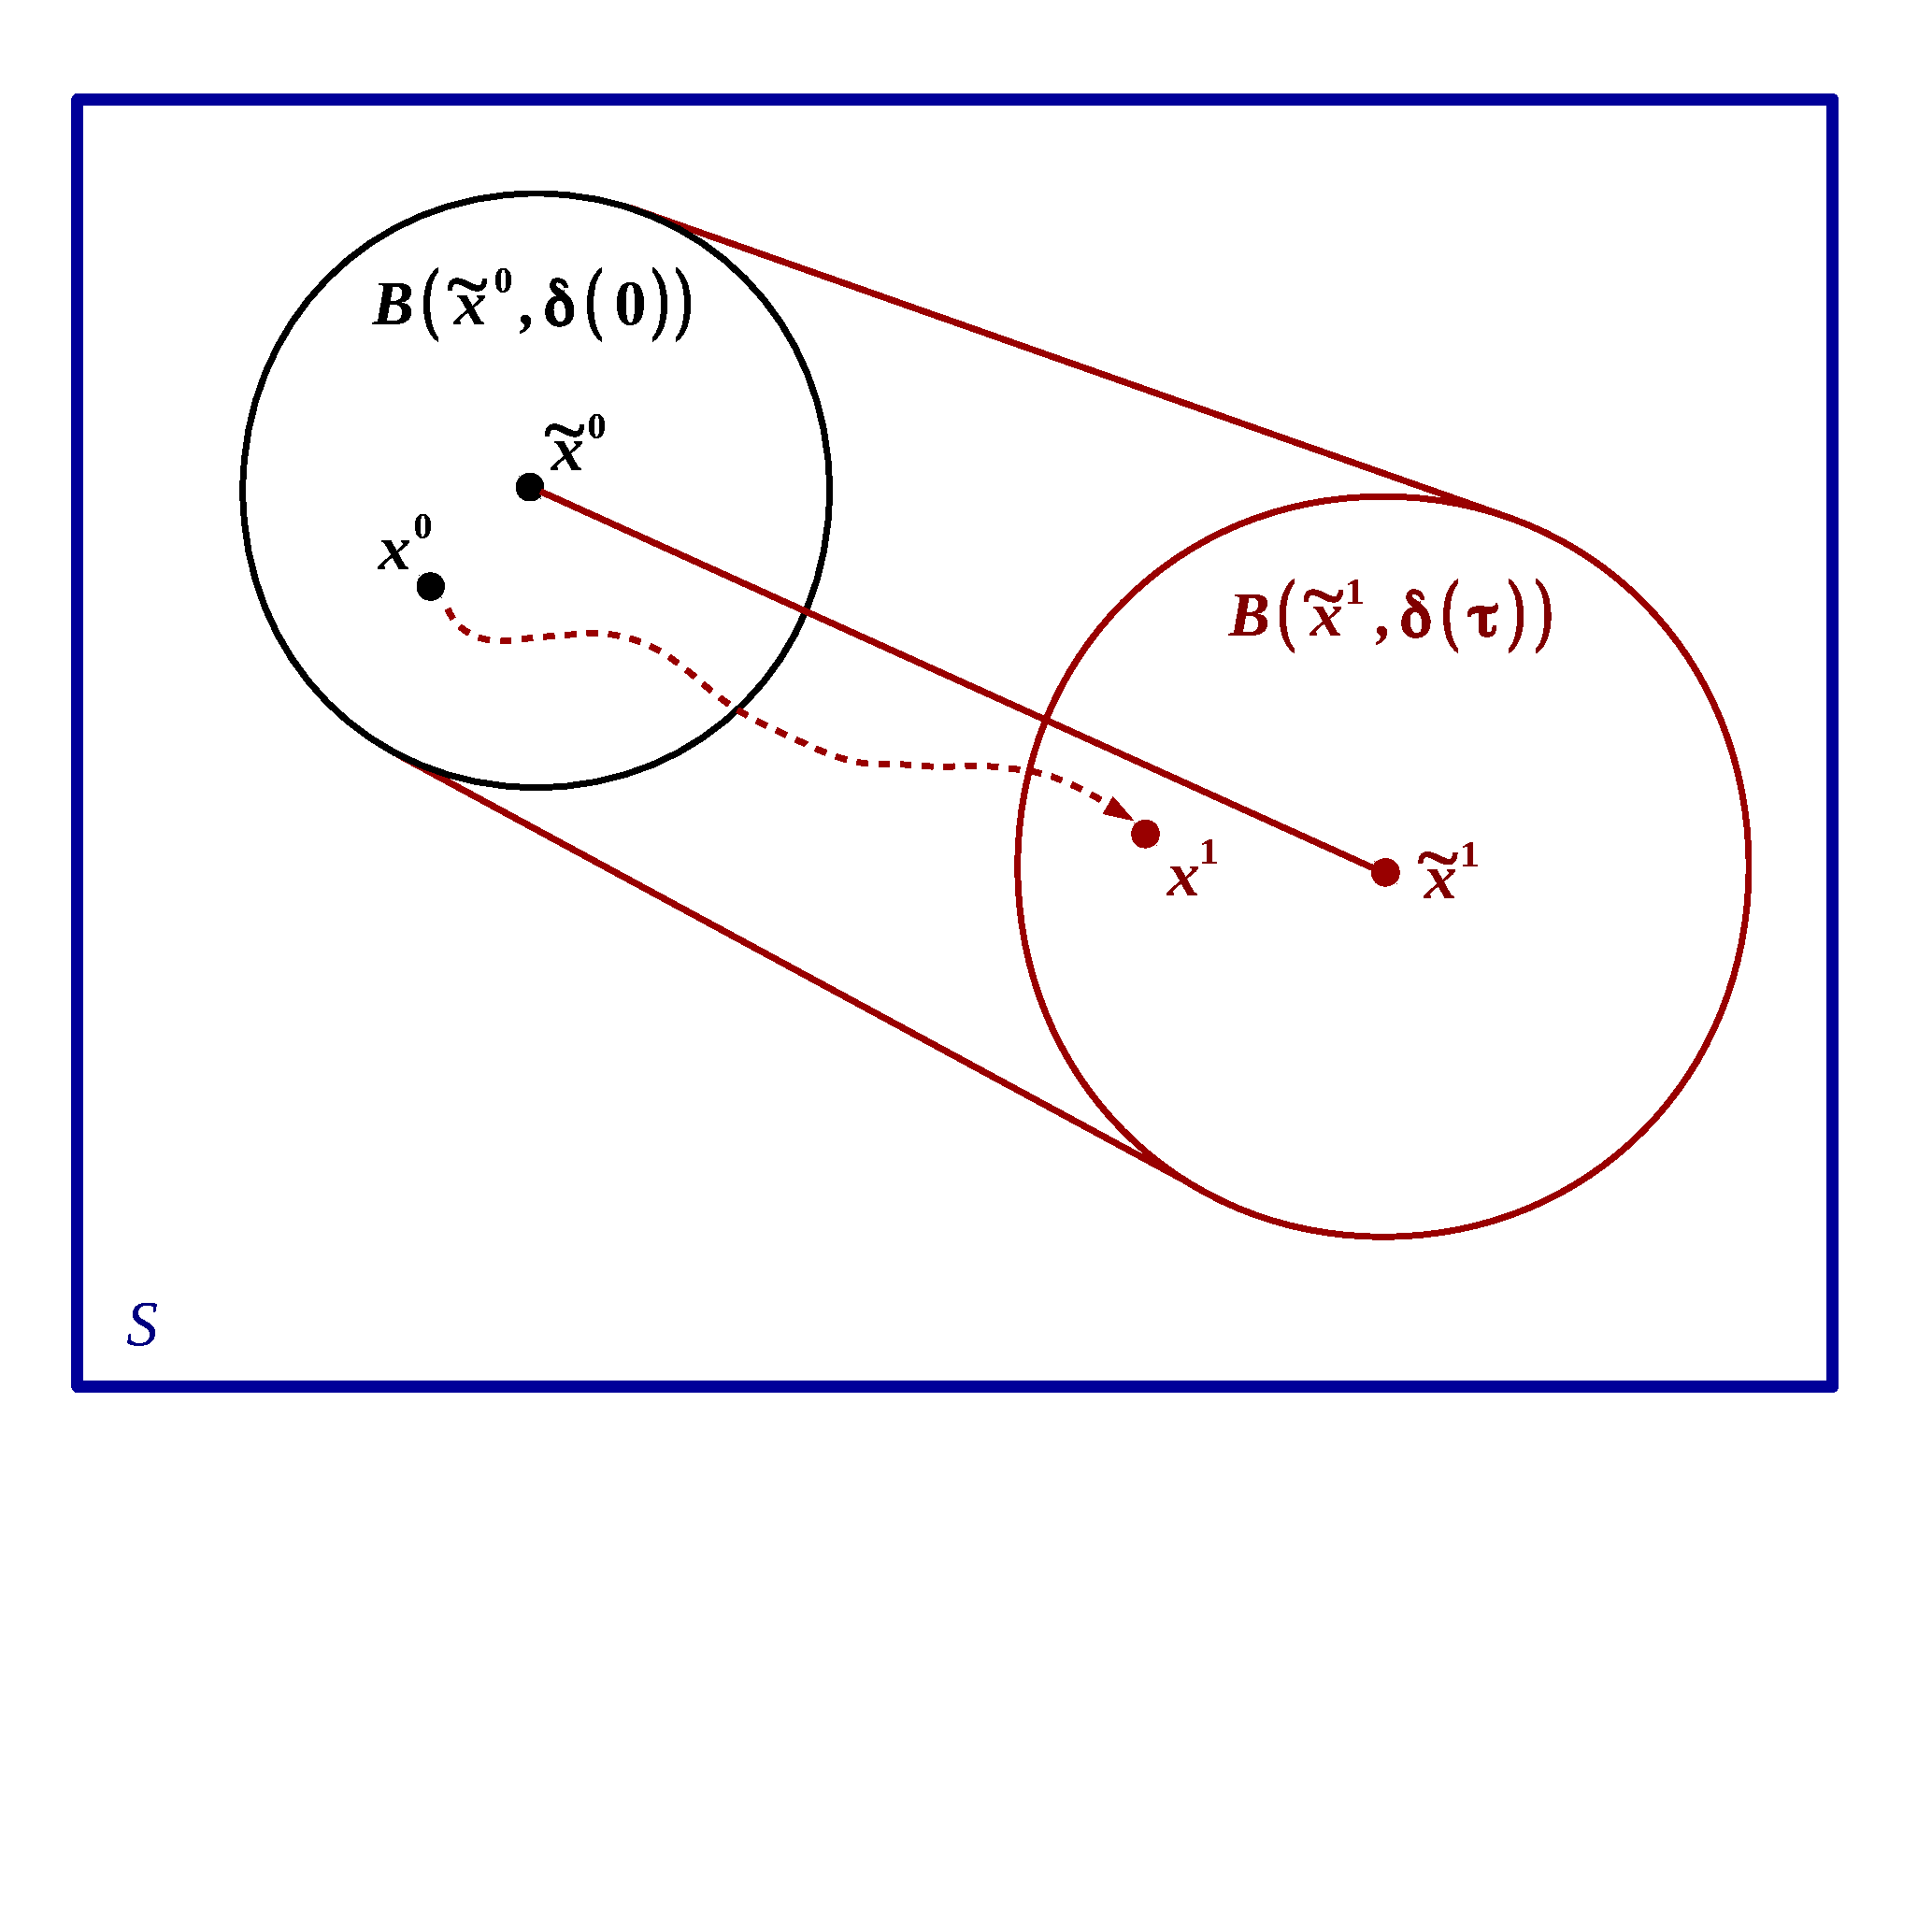
\includegraphics[width=0.49\textwidth,clip,trim = 0cm 9.5cm 0cm 0cm]{ball_image2.pdf}
%     % &
%     % 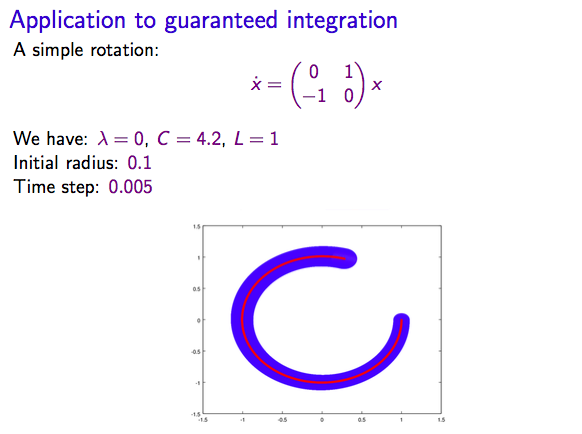
\includegraphics[width=0.49\textwidth]{rotation_Euler.png}
%     % \\
%     % (a) & (b)
% %  \end{tabular}
%   \caption{Illustration of Corollary \ref{cor:1_part4}, with $\tilde x_1 = \tilde{\phi}(\tau;\tilde{x}^0)$
%     and $x_1 = {\phi}(\tau;{x}^0)$.}
%   \label{fig:control_switch}
% \end{figure}
% 
% 
% \begin{corollary}\label{cor:1_part4}
% 
% Given an ODE system %\eqref{eq:sys_part4}
% satisfying (H0-H1), consider
% a point $\tilde{x}^0\in S$ and a real $\delta>0$ such that:
% \begin{enumerate}
% \item $B(\tilde{x}^0,\delta)\subseteq S$,
% \item $B(\tilde{\phi}(\tau;\tilde{x}^0),\delta(\tau))\subseteq S$, and
% \item $\frac{d^2(\delta(t))}{dt^2}>0$ for all $t\in [0,\tau]$.
% \end{enumerate}
% Then we have, for all $x^0\in B(\tilde{x}^0,\delta)$ and $t\in[0,\tau]$:\
% %
% %$\phi(t;x^0)\in B(\tilde{\phi}(t;\tilde{x}^0),\delta(t))\subseteq S$
% $\phi(t;x^0)\in S$.
% 
% 
% \end{corollary}
% \subsection{Sampled switched systems}\label{ss:switch}
% Let us consider the nonlinear switched system
% \begin{equation}
%  \dot  x(t) = f_{\sigma (t)}( x(t))
%  \label{eq:sys_part4}
% \end{equation}
% defined for all $t \geq 0$, where $ x(t) \in \mathbb{R}^n$ is the state
% of the system, $\sigma(\cdot) : \mathbb{R}^+ \longrightarrow U$ is the
% switching rule. The finite set $U = \{ 1, \dots , N \}$ is the set of
% switching {\em modes} of the system.  We focus on {\em sampled switched systems}:
% given a sampling period $\tau >0$, switchings will occur at times
% $\tau$, $2\tau$, \dots{} The switching rule~$\sigma(\cdot)$ is thus constant
% on the time interval $\lbrack (k-1) \tau , k \tau )$ for $k \geq 1$.
% For all $j\in U$, $f_j$ is a function from $\mathbb{R}^n$ to~$\mathbb{R}^n$.\\
% % We call ``\emph{pattern}'' a finite sequence of modes $\pi =
% % (i_1,i_2,\dots,i_k) \in U^k$.
% 
% We will denote by $\phi_\sigma(t; x^0)$ the
% solution at time~$t$ of the system:
% 
% \begin{equation}
% \begin{aligned}
%   \dot  x(t) & =  f_{\sigma (t)}( x(t)), \\
%    x(0) & =   x^0. \\
% %  \sigma(t) & =  j \in U \ \text{for} \ t
% %  \in \lbrack k\tau , (k+1)\tau ),\ \ k=0,1,\dots
% \end{aligned}
%  \label{eq:sampled-switch-sys}
% \end{equation}
% %
% 
% 
% Often, we will consider $\phi_\sigma(t;x^0)$ on the interval $0\leq t<\tau$ for which $\sigma(t)$ is equal to a constant, say $j\in U$. In this case, we will abbreviate $\phi_\sigma(t;x^0)$ as $\phi_j(t;x^0)$. We will also consider $\phi_\sigma(t;x^0)$ on the interval $0\leq t<k\tau$
% where $k$ is a positive integer, and
% $\sigma(t)$ is equal to a constant, say $j_{k'}$,
% on each interval
% $[(k'-1)\tau,k'\tau)$ with $1\leq k'\leq k$; in this case,
% we will abbreviate $\phi_\sigma(t;x^0)$ as $\phi_\pi(t;x^0)$,
% where $\pi$ is a sequence of $k$ modes (or ``pattern'') of the form
% $\pi=j_1\cdot j_2\cdot\dots\cdot j_k$.
% 
% We will assume that $\phi_\sigma$ is {\em continuous} at time $k\tau$ for all positive integer $k$.
% This means that there is no ``reset'' at time $k'\tau$ ($1\leq k'\leq k$);
% the value of
% $\phi_\sigma(t,x^0)$ for $t\in[(k'-1)\tau,k\tau]$
% corresponds to the solution of $\dot{x}(u)=f_{j_{k'}}(x(u))$  for $u\in [0,\tau]$
% with initial value $\phi_\sigma((k'-1)\tau;x^0)$.\\
% 
% More generally, given an initial point $\tilde{x}^0\in S$ and  pattern $\pi$ of $U^k$,
% we can define a ``(piecewise linear) approximate solution''
% $\tilde{\phi}_\pi(t;\tilde{x}^0)$ of $\phi_\pi$ at time $t\in[0,k\tau]$ as follows:
% \begin{itemize}
% \item $\tilde{\phi}_\pi(t;\tilde{x}^0) = t f_j(\tilde{x}^0) + \tilde{x}^0$ if $\pi=j\in U$, $k=1$ and $t\in[0,\tau]$, and
% 
% \item $\tilde{\phi}_{\pi}(k\tau+t;\tilde{x}^0) = t f_j(\tilde{z}) + \tilde{z}$
% with $\tilde{z}=\tilde{\phi}_{\pi'}((k-1)\tau;\tilde{x}^0)$, if $k\geq 2$,
% $t\in[0,\tau]$,
% $\pi=j\cdot \pi'$ for some $j\in U$ and $\pi'\in U^{k-1}$.
% \end{itemize}
% 
% %{\bf NB: } We suppose that all the intermediate points $\tilde{z}$ belong to $S$ (\`a pr\'eciser)???.\\
% 
% We wish to synthesize a safety control $\sigma$ for $\phi_{\sigma}$
% using the approximate functions $\tilde{\phi}_\pi$. %\eqref{eq:grossier_part4}.
% %
% Hypotheses (H0) and (H1), as defined in Section \ref{ss:ODE},
% are naturally extended to every mode $j$ of $U$, as well as
% definition of $T$, constants $L$, $C$ and~$\lambda$, definitions of
% $\tilde{\phi}_j$ and $\delta$ (see \cite{SNR17}). From a notation point of view,
% we will assign an index $j$ to symbols $\lambda, L, C,\dots$ in order to
% relate them to the dynamics of mode $j$.\\
% 
% Consider a point~$\tilde{x}^0\in S$, a positive real  $\delta$ %\geq \frac{C_j\tau}{|\lambda_j|}$ for all $j\in U$,
% and a pattern $\pi$ of length $k$.
% Let $\pi(k')$ denote the $k'$-th element (mode) of~$\pi$ for $1\leq k'\leq k$.
% Let us abbreviate
% the $k'$-th approximate point
% $\tilde{\phi}_{\pi}(k'\tau;\tilde{x}^{0})$
% as~$\tilde{x}_\pi^{k'}$ for $k'=1,...,k$,
% and let $\tilde{x}_\pi^{k'}=\tilde{x}^0$ for $k'=0$. It is easy to show that
% $\tilde{x}_\pi^{k'}$ can be defined recursively for $k'=1,...,k$, by:
% $\tilde{x}_\pi^{k'}=\tilde{x}_\pi^{k'-1}+\tau f_{j}(\tilde{x}_\pi^{k'-1})$
% with $j=\pi(k')$.
% 
% Let us now
% define the expression $\delta_\pi^{k'}$
% %(an upper bound on) the error associated to $\tilde{x}_\pi^{k'}$,
% %i.e. $\|\tilde{x}_\pi^{k'}- \phi_\pi(k'\tau;x^0)\|$.
% %Using repeatedly Theorem \ref{th:1_part4},
% %$\delta_{\pi}^{k'}$ can be defined recursively
% as follows:
% %\begin{itemize}
% %\item
% %(i.e., $\tilde{x}^{k'}=
% %\tilde{x}^{k'-1} +\tau f_{\pi(k')}(\tilde{x}^{k'-1})$).
% %\item
% For $k'=0$: $\delta_{\pi}^{k'}=\delta$,
% and for $1\leq k'\leq k$: $\delta^{k'}_{\pi}=\delta'_j(\tau)$
% where $\delta'$ denotes $\delta^{k'-1}_{\pi}$, and $j$ denotes
% $\pi(k')$.
% %\end{itemize}
% Likewise, for $0\leq t\leq k\tau$, let us
% define the expression $\delta_{\pi}(t)$  as follows:
% %(an upper bound on) the
% %global error associated to $\tilde{\phi}_\pi(t;\tilde{x}^0)$
% %(i.e.~$\|\tilde{\phi}_\pi(t;\tilde{x}^0)- \phi_\pi(t;x^0)\|$).
% %Using Theorem \ref{th:1_part4},
% %$\delta_{\pi}(t)$ can be defined itself as follows:
% \begin{itemize}
% \item for $t=0$:\ $\delta_\pi(t)=\delta$,
% \item for $0<t\leq k\tau$:\
% $\delta_{\pi}(t)=\delta'_{j}(t')$ with
% $\delta'=\delta_\pi^{\ell-1}$, $j=\pi(\ell)$,
% $t'=t-(\ell-1)\tau$ and
% $\ell=\lceil \frac{t}{\tau}\rceil$.
% \end{itemize}
% Note that, for $0\leq k'\leq k$, we have:
% $\delta_{\pi}(k'\tau)=\delta_\pi^{k'}$. We have
% \begin{theorem}\label{th:safety}
%   Given a sampled switched system satisfying (H0-H1), consider a
%   point~$\tilde{x}^0\in S$, a positive real $\delta$ and a pattern
%   $\pi$ of length $k$ such that, for all $1\leq k'\leq k$:
%   \begin{enumerate}
%   \item $B(\tilde{x}_\pi^{k'}, \delta_{\pi}^{k'}) \subseteq S$ and
%   \item $\frac{d^2(\delta'_j(t))}{dt^2}>0$ for all $t\in [0,\tau]$,
%     with $j=\pi(k')$ and $\delta'=\delta_\pi^{k'-1}$.
%   \end{enumerate}
%   Then we have, for all $x^0\in B(\tilde{x}^0,\delta)$ and $t\in
%   [0,k\tau]$:\ \ $\phi_{\pi}(t;x^0)\in S$.
% \label{prop:1bis_part4}
% \end{theorem}
% 
% \begin{remark}
%   In Theorem~\ref{prop:1bis_part4}, we have supposed that the step size $h$
%   used in Euler's method was equal to the sampling period $\tau$ of
%   the switching system.  Actually, in order to have better
%   approximations, it is often convenient to take a {\em fraction} of
%   $\tau$ as for $h$ (\textit{e.g.}, $h=\frac{\tau}{10}$).  Such a
%   splitting is called ``sub-sampling'' in numerical methods.
% \end{remark}
% 
% Consider now a compact set $R$, called ``recurrence set'', contained
% in the safety set $S\subset\mathbb{R}^n$ ($R\subseteq S$). We are
% interested in the synthesis of a control such that: starting from any
% initial point $x\in R$, the controlled trajectory always returns to
% $R$ within a bounded time while never leaving $S$.
% 
% \begin{corollary}
%   \label{cor:cont}
%   Given a switched system satisfying (H0-H1), consider a positive real
%   $\delta$ and a finite set of points $\tilde{x}_1,\dots\tilde{x}_m$
%   of $S$ such that all the balls $B(\tilde{x}_i,\delta)$ cover~$R$ and
%   are included into~$S$ (\textit{i.e.}, $R\subseteq
%   \bigcup_{i=1}^mB(\tilde{x}_i,\delta)\subseteq S$).
% 
%   Suppose furthermore that, for all $1\leq i\leq m$, there exists a
%   pattern $\pi_i$ of length $k_i$ such that:
%   \begin{enumerate}
%     % \item $B(\tilde{\phi}_{\pi_i}(k'\tau;\tilde{x}_i),
%     %   \delta_{\pi_i}(k'\tau)) \subseteq S$,
%   \item $B((\tilde{x}_i)_{\pi_i}^{k'},\delta_{\pi_i}^{k'}) \subseteq
%     S$, for all $k'=1,\dots,k_i-1$
% %
% \item
% %$B(\tilde{\phi}_{\pi_i}(k_i\tau;\tilde{x}_i), \delta_{\pi_i}(k_i\tau)) \subseteq R.$
%   $B((\tilde{x}_i)_{\pi_i}^{k_i}, \delta_{\pi_i}^{k_i}) \subseteq R.$
% %
% \item $\frac{d^2(\delta'_j(t))}{dt^2}>0$ with $j=\pi_i(k')$ and
%   $\delta'=\delta_{\pi_i}^{k'-1}$, for all $k'\in\{1,...,k_i\}$ and
%   $t\in [0,\tau]$.
% %$\frac{d^2(\delta'_j(t)}{dt^2}>0$ for all $t\in [0,\tau]$, $j\in U$ and $\delta'\in [\delta]$.
% \end{enumerate}
% These properties induce a control $\sigma$\footnote{Given an initial
%   point $x\in R$, the induced control $\sigma$ corresponds to a
%   sequence of patterns $\pi_{i_1},\pi_{i_2},\dots$ defined as follows:
%   Since $x\in R$, there exists a a point $\tilde{x}_{i_1}$ with $1\leq
%   i_1\leq m$ such that $x\in B(\tilde{x}_{i_1},\delta)$; then using
%   pattern $\pi_{i_1}$, one has: $\phi_{\pi_{i_1}}(k_{i_1}\tau;x)\in
%   R$. Let $x'=\phi_{\pi_{i_1}}(k_{i_1}\tau;x)$; there exists a point
%   $\tilde{x}_{i_2}$ with $1\leq i_2\leq m$ such that $x'\in
%   B(\tilde{x}_{i_2},\delta)$, etc.}
% %
% which guarantees
% %Let $k_{max}=\max_{i=1,\dots,m}\{k_i\}$.
% \begin{itemize}
% \item (safety): if $x\in R$, then $\phi_{\sigma}(t;x) \in S$ for all
%   $t\geq 0$, and
% \item (recurrence): if $x\in R$ then $\phi_{\sigma}(k\tau;x)\in R$ for
%   some $k\in\{k_1,\dots,k_m\}$.
% \end{itemize}
% %
% \label{prop:ter1_part4}
% \end{corollary}
% 
% Corollary~\ref{prop:ter1_part4} gives the theoretical foundations of the
% following method for synthesizing $\sigma$ ensuring recurrence in $R$
% and safety in $S$:
% \begin{itemize}
% \item we (pre-)compute $\lambda_j, L_j, C_j$ for all $j\in U$;
% \item we find $m$ points $\tilde{x}_1,\dots\tilde{x}_m$ of $S$ and
%   $\delta>0$ such that $R\subseteq \bigcup_{i=1}^m
%   B(\tilde{x}_i,\delta)\subseteq S$;
% %for some $\delta>0$;%\geq \frac{C_j\tau}{\lambda}$;
% \item we find $m$ patterns $\pi_i$ ($i=1,...,m$) such that conditions
%   1-2-3 of Corollary~\ref{prop:ter1_part4} are satisfied.
% \end{itemize}
% %
% A covering of $R$ with balls as stated in Corollary~\ref{prop:ter1_part4} is
% illustrated in Figure~\ref{fig:post_part4}~(a).  The control synthesis
% method based on~Corollary \ref{prop:ter1_part4} is illustrated in
% Figure~\ref{fig:post_part4}~(b).
% %(left)
% %together with an illustration of method of \cite{NL_minimator} (right).
% 
% 
% 
% 
% %  \begin{column}{0.48\textwidth}
%  \begin{figure}[t]
%  \centering
% \begin{tabular}{cc}
% 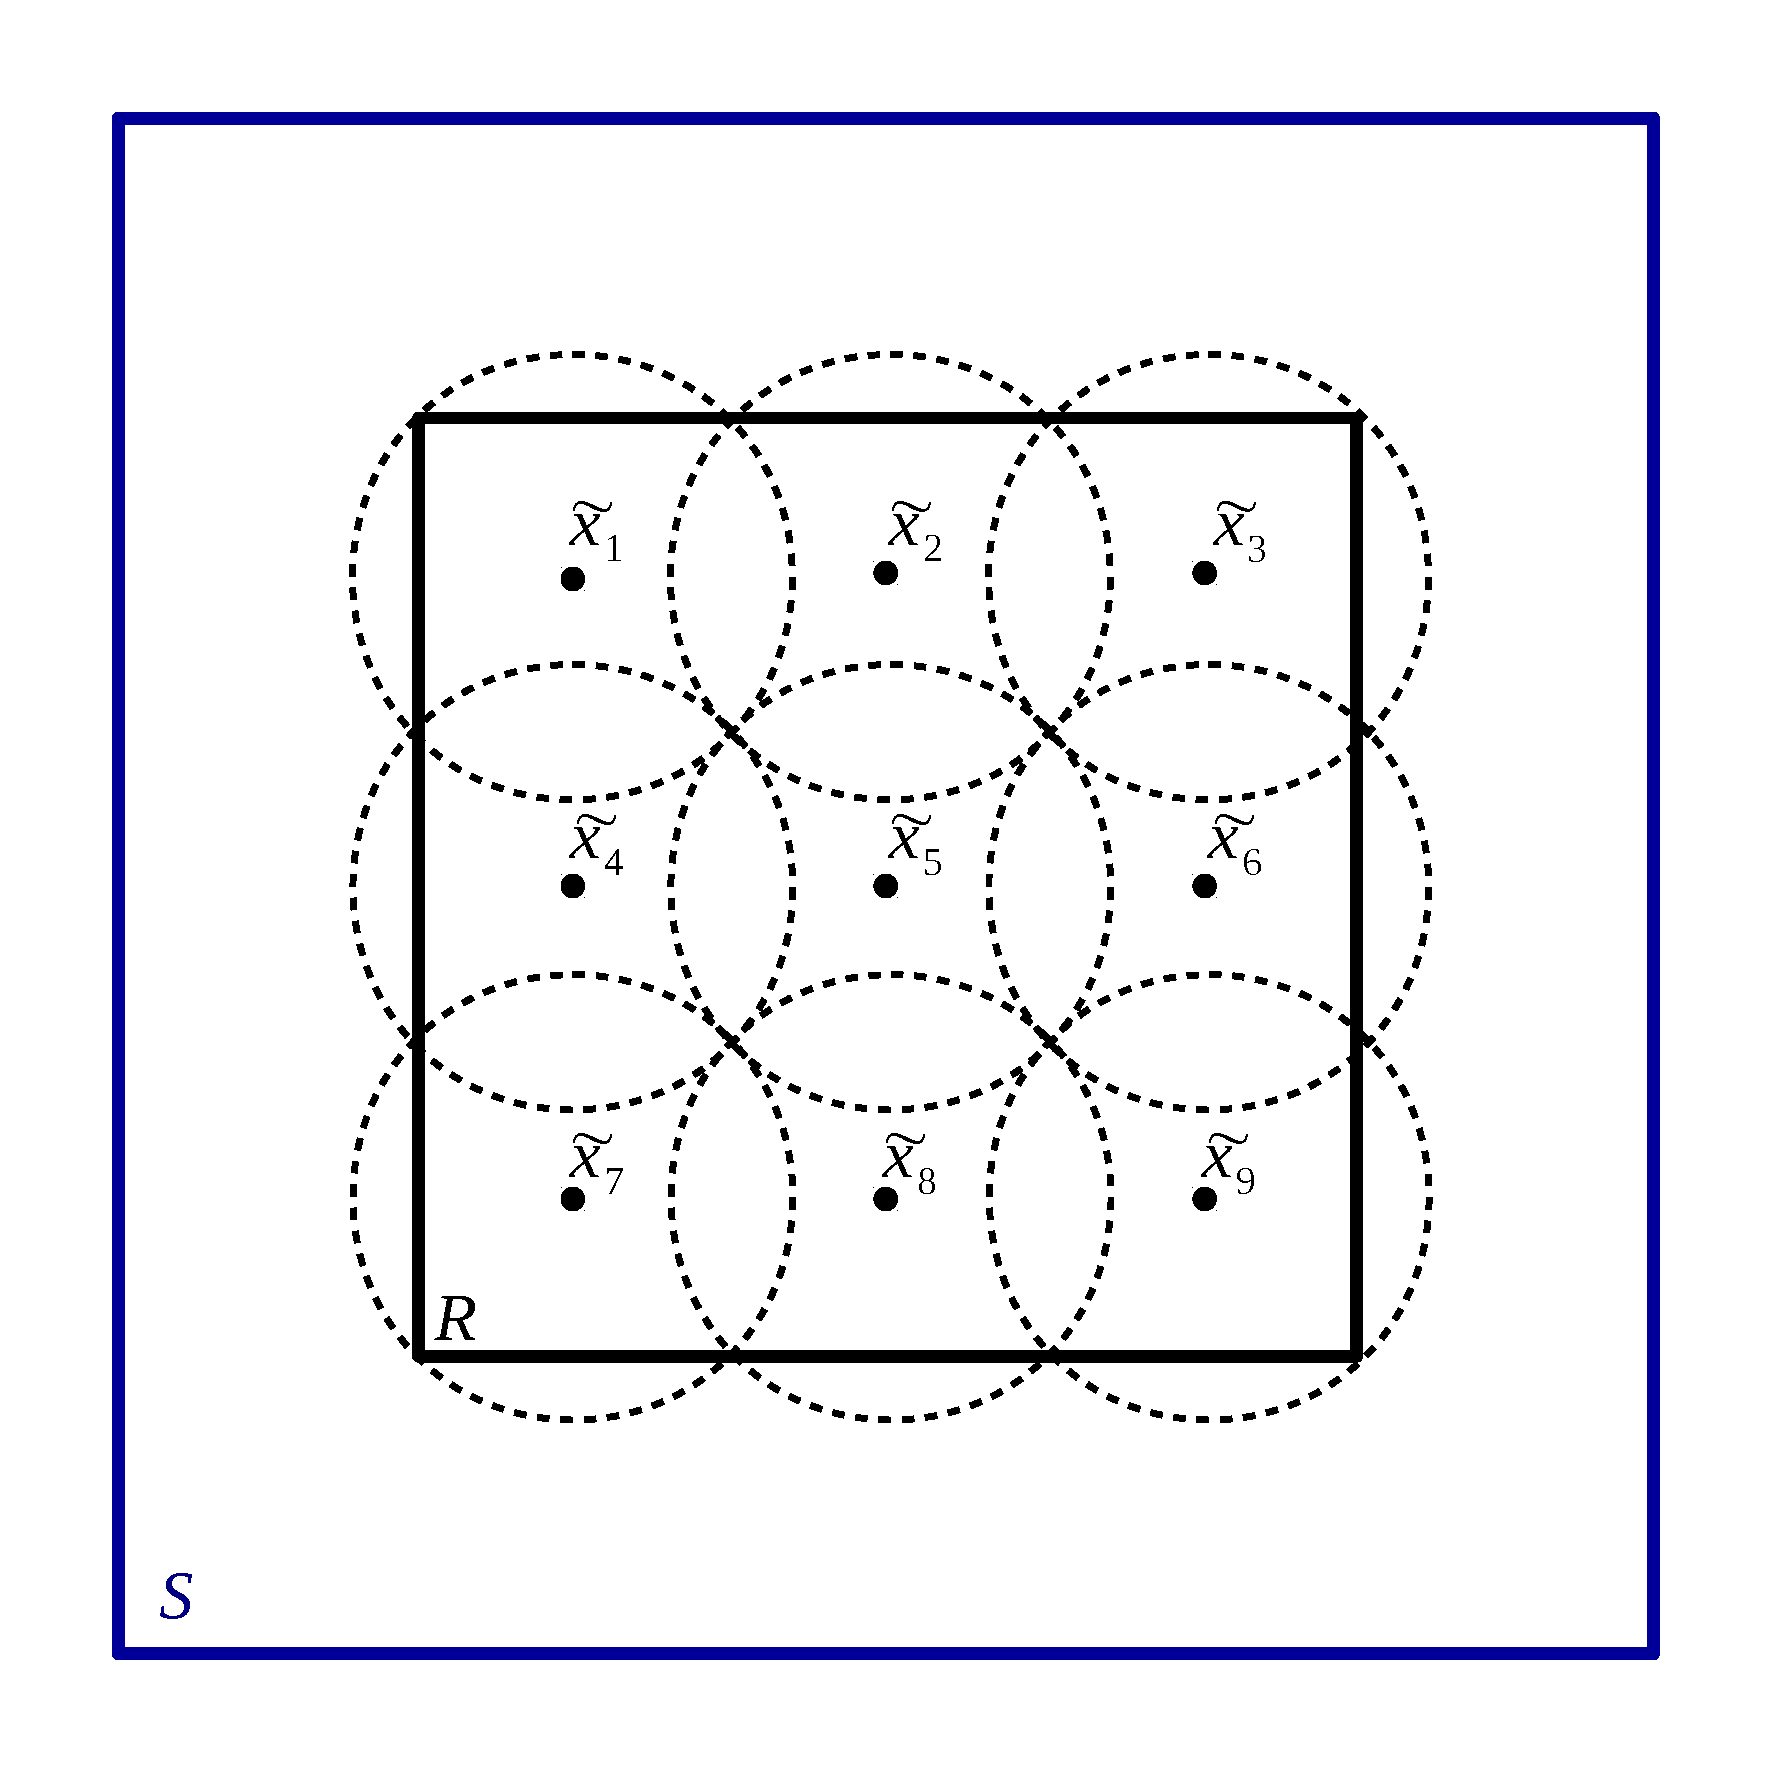
\includegraphics[width=0.42\textwidth,clip,trim=1cm 0cm 1cm 0cm]{tilingball2.pdf}
% &
%  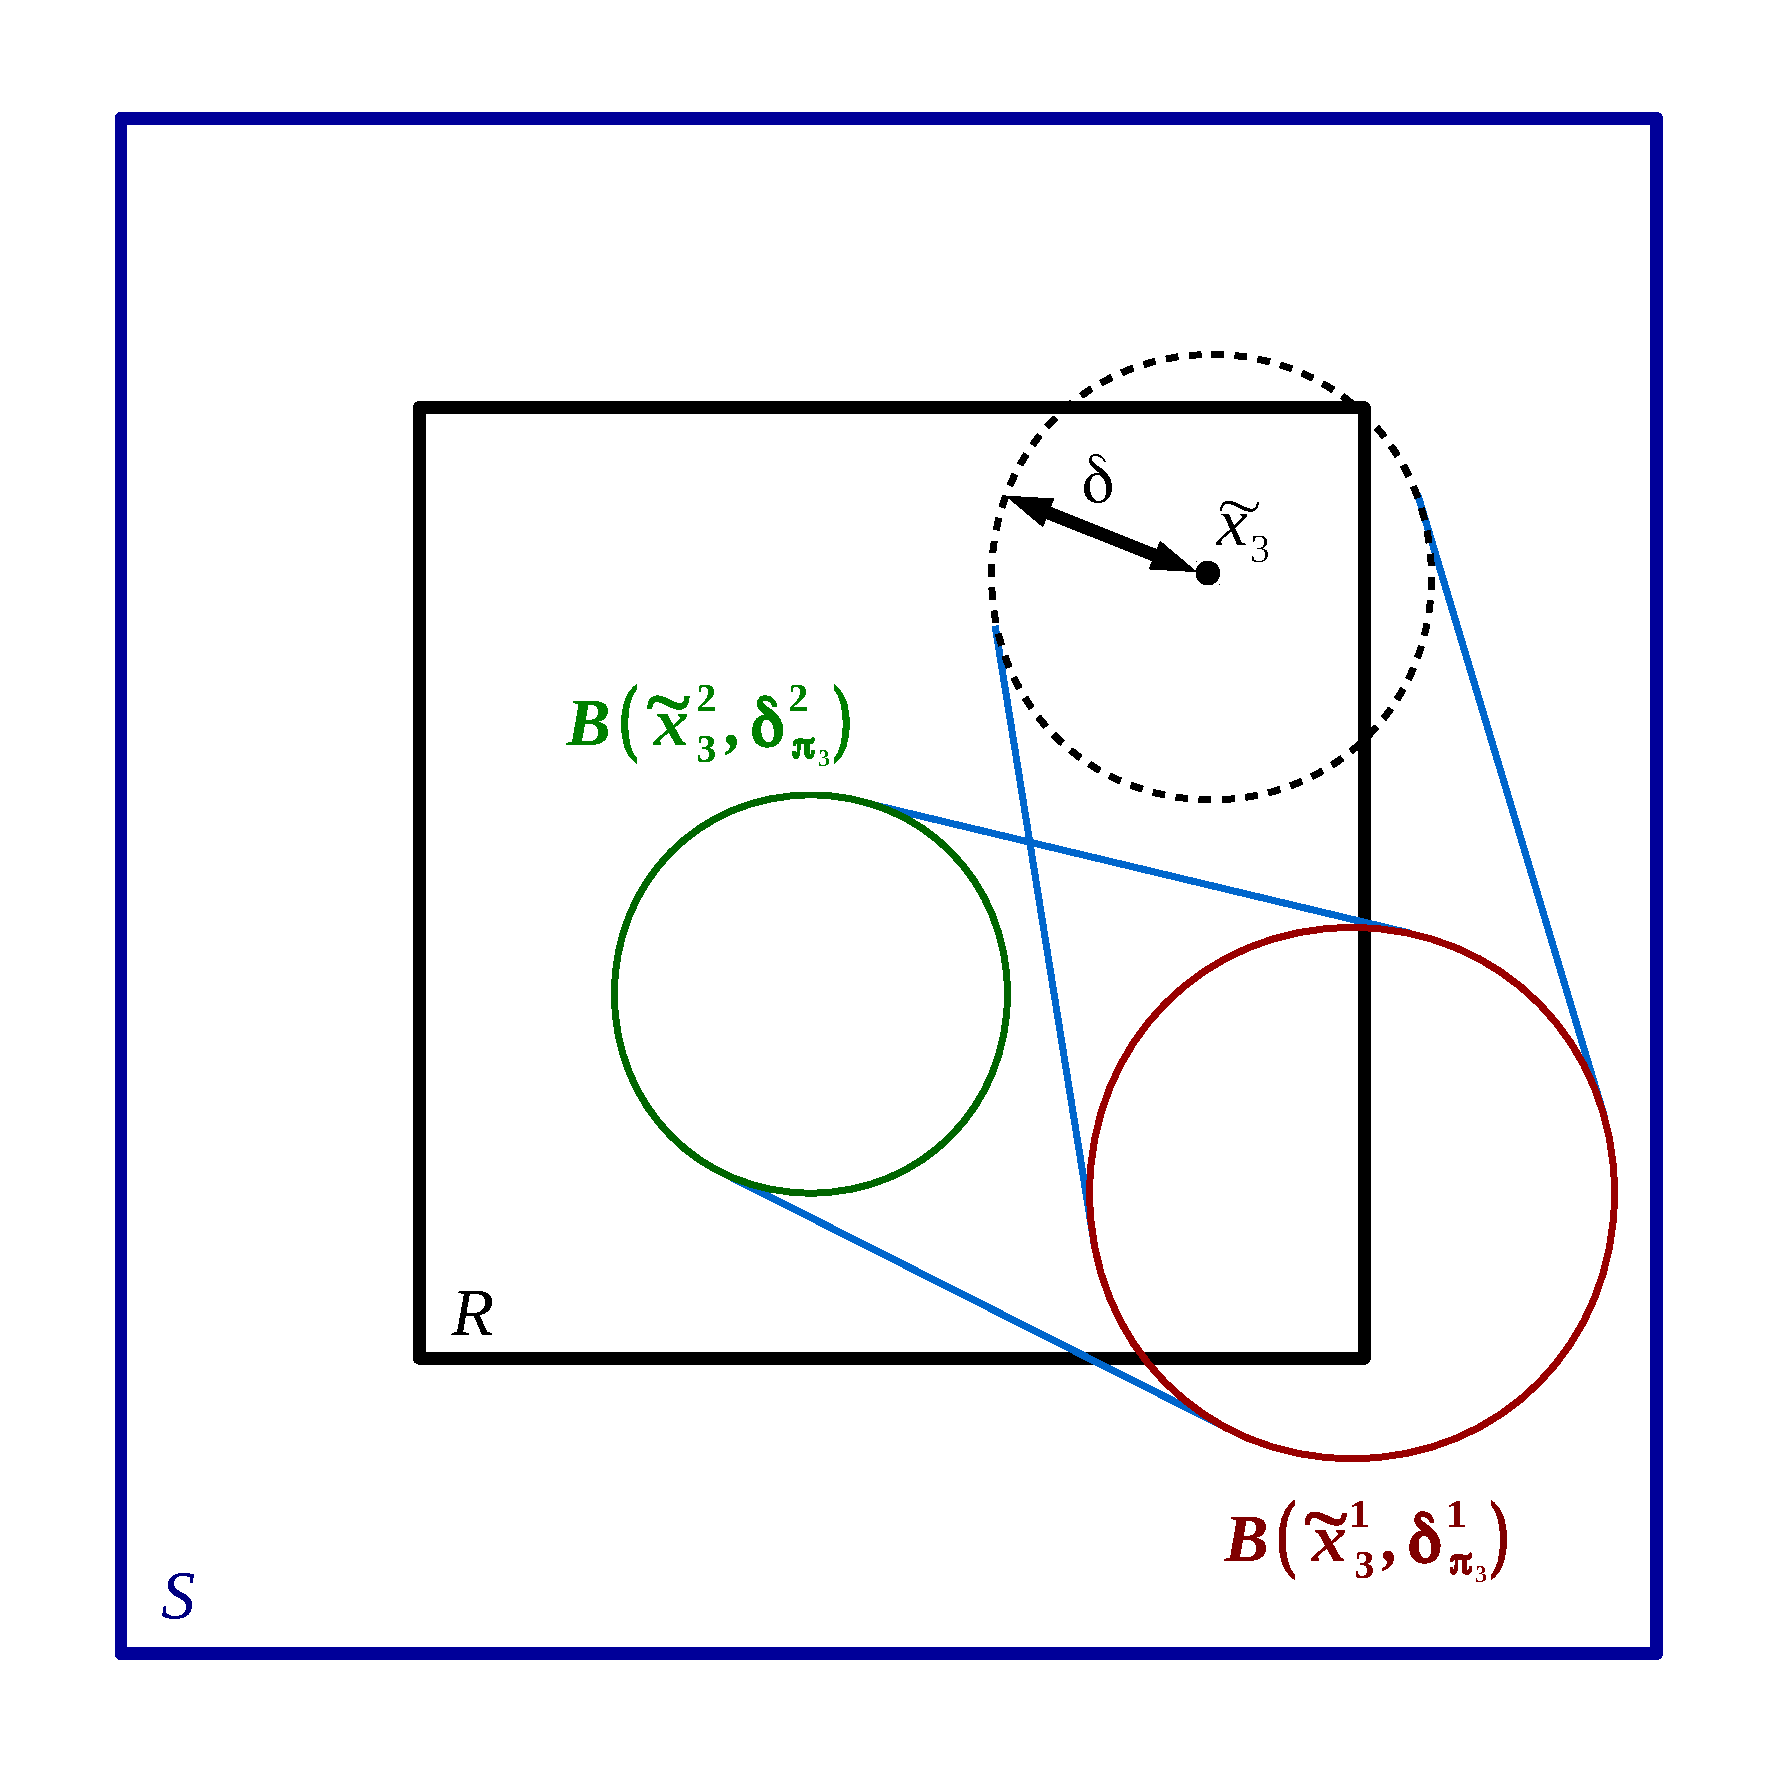
\includegraphics[width=0.42\textwidth,clip,trim=1cm 0cm 1cm 0cm]{tilingballimage.pdf}
%  \\
%  (a) & (b)
% \end{tabular}
% \caption{(a): A set of balls covering $R$ and contained in $S$. (b): Control of ball $B(\tilde x_3,\delta)$ with Euler-based method.}
% \label{fig:post_part4}
% \end{figure}
% 
% 


In this chapter, we extend the results of the previous chapter to 
systems subject to disturbances and varying parameters. 
The introduction of varying parameters is an important step 
to the applicability of the method because real systems 
can be identified to switched system of the form \eqref{eq:switched_system0}
up to a certain (finite) precision. We also present how disturbances can be used to 
perform distributed (also called compositional) control synthesis.
Provided that the modes do not affect each dimension of the system, 
system \eqref{eq:switched_system0} can be rewritten as two sub-systems with independent control modes, 
but sharing some state variables. Those shared state variables 
can be viewed as disturbances, and using a method close to assume-guarantee reasoning \cite{???},
we synthesize two controllers, much cheaper to compute than a centralized one.






\section{Distributed control using zonotopes}
\paragraph{Plan}
%
The structure of this section is as follows.  The~class of 
discrete-time systems
considered and some preliminary definitions are given in
Section~\ref{sec:switch}.  Our~symbolic approach, which is based on
the tiling of the state space and backward reachability, is explained
in Section~\ref{sec:tiling}.  In~Section~\ref{sec:one-step},
we~present a centralized method to synthesize a controller based on a
``generate-and-test'' tiling procedure.  A~distributed approach is
then given in Section~\ref{sec:distr}, where we introduce a state
over-approximation technique in order to avoid the use of non-local
information by the subsystem controllers.  For both methods, we
provide reachability and stability guarantees on the controlled
trajectories of the system. Our~distributed approach is applied
in~Section~\ref{sec:case_study0} on a real case study of temperature
control in a building with $11$ rooms and $2^{11}=2048$ switching
modes of control.   The~method is extended in the 
continuous-time framework in Section~\ref{sec-continuous}.
%We~conclude in Section~\ref{sec:conc}.

%\fbox{+ Section~\ref{sec-nonlinear} continuous
%  non-linear case + other case study}




\subsection{State-dependent Switching Control}\label{sec:switch}
We first consider the \emph{discrete-time} setting.
The~time~$t$ then takes its values in~$\mathbb{N}$.
\subsubsection{Control modes}\label{ss:modes}
Consider the following discrete-time system with \emph{finite control}:
\begin{xalignat*}2
 x_1(t+1) &= f_1(x_1(t),x_2(t),u_1)  &
 x_2(t+1) &= f_2(x_1(t),x_2(t),u_2)
\end{xalignat*}
where $x_1$ (resp.~$x_2$) is the first (resp.~second) component
of the state vector, and takes its values
in $\mathbb{R}^{n_1}$ (resp.~$\mathbb{R}^{n_2}$), 
and where $u_1$ (resp.~$u_2$) is
the first (resp.~second) component of the control \emph{mode},
and takes its values in the \emph{finite} set~$U_1$ (resp.~$U_2$).
We~will often write~$x$ for~$(x_1,x_2)$, $u$~for~$(u_1,u_2)$,
and $n$ for~$n_1+n_2$.
We~will also abbreviate the set $U_1\times U_2$ as~$U$.
%
Let~$N_1$ (resp.~$N_2$) by the cardinality
of~$U_1$ (resp.~$U_2$), and $N=N_1 \cdot N_2$ be the cardinality of~$U$.

More generally, we abbreviate the discrete-time system under
the form:
%
\[
x(t+1)=f(x(t),u)
\]
where $x$ is a vector state variable, taking
its values in $\mathbb{R}^n=\mathbb{R}^{n_1}\times \mathbb{R}^{n_2}$,
and where $u$ is of the form $(u_1,u_2)$,
where $u_1$~takes its values in~$U_1$ and $u_2$ in~$U_2$.

%Let $n=n_1+n_2$, be the dimension of the state space.
In this context, we are interested by the following \emph{centralized}
control-synthesis problem: at~each discrete-time~$t$, select some
appropriate mode $u\in U$ in order to satisfy a given
property. In~this paper we focus on \emph{state-dependent} control,
which means that, at each time~$t$, the~selection of the value of~$u$
is performed by only considering the values of~$x(t)$.
%
In~a \emph{distributed} setting, the control-synthesis problem
consists in selecting the value of~$u_1$ in~$U_1$ according to the
value of~$x_1(t)$ \emph{only}, and the value of~$u_2$ in~$U_2$
according to the value of~$x_2(t)$ \emph{only}.

The properties that we consider are \emph{reachability} properties:
given a set~$S$ and a set~$R$, we~look for a control which
steers any element of~$S$ into~$R$ in a bounded number of steps.
We~also consider \emph{stability} properties, requiring that
once the state~$x$ of the system is in~$R$ at time~$t$,
the control will maintain it in~$R$ indefinitely.
%at $t+1, t+2,\cdots$.
%
Actually, given a state set~$R$, we will present a method that
does not start from a given set~$S$, but \emph{constructs}~it,
together with a control that steers all the elements
of~$S$ to~$R$ within a bounded number of steps
%\fbox{bounded time? (for continuous case)}
($S$~can be seen as a ``capture set'' of~$R$).
%%nFurthermore, the method can also be used to
%construct a control which makes $R$ stable.\\

In this paper, we consider that $R$ and~$S$ are ``rectangles''
of the state space.
More precisely, $R=R_1\times R_2$ is a rectangle of reals, i.e.,
$R$~is a product of $n$ closed intervals of reals,
%${\cal I}(\mathbb{R})\times{\cal I}(\mathbb{R})$
and $R_1$ (resp.~$R_2$) is a product of~$n_1$ (resp.~$n_2$) closed intervals
of reals.
Likewise, we assume that $S=S_1\times S_2$ is a rectangular
sub-area of the state space.
%\footnote{In the following, for the sake of simplicity, we will often assume 
%implicitly
%that $n_1=n_2=1$ and $n=2$, and will use the terminology of ``rectangles'' 
%for $R$ and $S$, and ``intervals'' for $R_1,R_2,S_1,S_2$.???}\\
%The \emph{(one-step backward reachability state-dependent) centralized control  problem} for $R$
%consists in finding a set $S$ %(containing $R$) 
%such that,
%for each $x\in R$ there exists~$u\in U$
%with:
%
%$f(x,u)\in R.$
%
%The \emph{(one-step backward reachability state-dependent) distributed control  problem} for $R$
%consists in finding a set $S=S_1\times S_2$ 
%(containing $R$) 
%such that,
%for each $x_1\in S_1$ there exists $u_1\in U_1$ with
%
%$\forall x_2\in S_2\ f_1(x_1,x_2,u_1)\in R_1$, and\\
%
%for each $x_2\in S_2$ there exists~$u_2\in U_2$ with:
%
%$\forall x_1\in S_1\ f_2(x_1,x_2,u_2)\in R_2$.\\
%\footnote{Actually, we will focus on sets which contain $S$
%(``capture set'')}
\begin{example}\label{ex:spec}
The centralized and distributed approaches will be illustrated by the
example of a two-room apartment, heated by one heater in each room
(adapted from~\cite{girard2012low}). In~this example, the~objective is
to control the temperature of both rooms. There~is heat exchange
between the two rooms and with the environment. The~\emph{continuous}
dynamics of the system is given by the equation:
\[
\dot{\left(
  \begin{matrix}T_1 \\ T_2 \end{matrix}
  \right)} =
\left(
\begin{matrix}
  - \alpha_{21} - \alpha_{e1}-\alpha_f{u_1} \hskip-5mm& \alpha_{21} \\
    \alpha_{12}        &-\alpha_{12}-\alpha_{e2} - \alpha_f u_2
\end{matrix}
\right)
\left(
\begin{matrix}T_1 \\ T_2 \end{matrix} \right) +
\left(
\begin{matrix} 
  \alpha_{e1} T_e + \alpha_f T_f { u_1} \\
  \alpha_{e2}T_e + \alpha_fT_fu_2
\end{matrix}
\right).
\]
%
Here $T_1$ and $T_2$ are the temperatures of the two rooms, and the
state of the system corresponds to $T=(T_1,T_2)$.  The~control mode
variable~$u_1$ (respectively~$u_2$) can take the values $0$ or~$1$,
depending on whether the heater in room~1 (respectively room~2) is
switched off or~on (hence~$U_1=U_2=\{0,1\}$).  Hence, here
$n_1=n_2=1$, $N_1=N_2=2$, and $n=2$ and $N=4$.

Temperature~$T_e$ corresponds to the temperature of the environment,
and $T_f$ to the temperature of the heaters.
%
 The values of the different parameters are as follows:
 $\alpha_{12} = 5 \times 10^{-2}$, $\alpha_{21} = 5 \times 10^{-2}$,
 $\alpha_{e1} = 5 \times 10^{-3}$, $\alpha_{e2} = 5 \times 10^{-3}$,
 $\alpha_{f} = 8.3 \times 10^{-3}$, $T_e = 10$ and $T_f = 35$.

We suppose that the heaters can be switched periodically at sampling
instants $\tau$, $2\tau$,~... (here,~$\tau=5s$).  By~integration of
the continuous dynamics between $t$ and~$t+\tau$, the~system can be
easily put under the desired \emph{discrete-time} form:
\begin{xalignat*}2
T_1(t+1) &= f_1(T_1(t),T_2(t),u_1) 
&
T_2(t+1) &= f_2(T_1(t),T_2(t),u_2)
\end{xalignat*}
where $f_1$ and $f_2$ are affine functions.


Given an objective rectangle for $T=(T_1,T_2)$ of the form $R=\lbrack
18.5 , 22 \rbrack \times \lbrack 18.5 , 22 \rbrack$, the control
synthesis problem is to find a rectangular capture set~$S$ (as large as
possible) from which one can steer the state~$T$ to~$R$
(``reachability''), and then maintai $T$ within~$R$ for ever
(``stability'').
%((see Section \ref{ss:special}).see Section \ref{ss:special}).
\end{example}




\subsubsection{Control patterns}
It is often easier to design a control of the system using several
applications of~$f$ in a row rather than using just a single
application of~$f$ at each time.  We~are thus led to the notion of
``macro-step'', and ``control pattern''.
%
A \emph{(control) pattern $\pi=(\pi_1,\pi_2)$ of length~$k$} 
is a sequence of modes defined recursively~by:
\begin{enumerate}
\item $\pi$ is of the form $(u_1,u_2)\in U_1\times U_2$ if $k=1$,
\item $\pi$ is of the form $(u_1\cdot \pi'_1,u_2\cdot \pi'_2)$,
where $u_1$ (resp. $u_2$) is in $U_1$ (resp. $U_2$),
and $(\pi'_1,\pi'_2)$ is a (control) pattern of length $k-1$ if $k\geq 2$.
\end{enumerate}

The set of patterns of length~$k$ is denoted by $\Pi^k$ (for length
$k=1$, we~have $\Pi^1=U$). Likewise, for $k\geq 1$, we denote by $\Pi_1^k$
(resp.~$\Pi_2^k$) the set of sequences of $k$ elements of~$U_1$
(resp.~$U_2$).

For a system defined by $x(t+1)=f(x(t),(u_1,u_2))$ and a pattern
$\pi=(\pi_1,\pi_2)$ of length~$k$, one~can  recursively define
$x(t+k)=f(x(t),(\pi_1,\pi_2))$ with ${(\pi_1,\pi_2)\in \Pi^k}$,~by:
\begin{enumerate}
\item $f(x(t),(\pi_1,\pi_2))=f(x(t),(u_1,u_2))$, if $(\pi_1,\pi_2)$ is
  a pattern of length $k=1$ of the form $(u_1,u_2)\in U$,
\item $f(x(t),(\pi_1,\pi_2))=f(f(x(t),(\pi'_1,\pi'_2)),(u_1,u_2))$, if
  $(\pi_1,\pi_2)$ is a pattern of length $k\geq 2$ of the form
  $(u_1\cdot\pi'_1,u_2\cdot\pi'_2)$ with $(u_1,u_2)\in U$ and
  ${(\pi'_1,\pi'_2)\in \Pi^{k-1}}$.
\end{enumerate}
One defines $(f(x,\pi))_1\in \mathbb{R}^{n_1}$ and $(f(x,\pi))_2\in
\mathbb{R}^{n_2}$ to be the first and second components of $f(x,\pi)\in
\mathbb{R}^{n_1}\times\mathbb{R}^{n_2}=\mathbb{R}^{n}$, i.e:
$f(x,\pi)=((f(x,\pi))_1,f(x,\pi)_2)$.


In the following, we fix an upper bound $K\in\mathbb{N}$ 
on the length of patterns.  The~value of~$K$ can be seen as a maximum
number of time steps, for which we compute the future behaviour of the
system~(``horizon'').
%
%It is also convenient to  assume given the existence of a tiling 
%${\cal R}^0=\{r^0_{i,j}\}_{i\in I_1^0, j\in I_2^0}$ of $R$ such that
%$\forall (i,j)\in I_1^0\times I_2^0\ $ of $R$.\\
%(hence a tiling ${\cal S}$ of $S=R+(a,a)$, for any $a\geq 0$).\\
%
We~denote by~$\Pi_1^{\leq K}$ 
(resp.~$\Pi_2^{\leq K}$)
the expression $\bigcup_{1\leq k \leq K}\Pi_1^k$ 
(resp.~$\bigcup_{1\leq k \leq K} \Pi_2^k$).
Likewise, we~denote by $\Pi^{\leq K}$
the expression $\bigcup_{1\leq k \leq K} \Pi^k$.







\subsection{Control Synthesis Using Tiling}\label{sec:tiling}
\subsubsection{Tiling}\label{ss:cent0}
Let $R=R_1\times R_2$
be a rectangle.
We say that $\cal  R$
is a \emph{(finite rectangular) tiling} of
$R$ if $\cal  R$ is of the form
$\{r_{i_1,i_2}\}_{i_1\in I_1, i_2\in I_2}$,
where 
$I_1$ and $I_2$ are given finite sets of positive integers, 
each $r_{i_1,i_2}$ is a sub-rectangle of $R$ of the form
$r_{i_1}\times r_{i_2}$, and $r_{i_1}, r_{i_2}$ 
are closed sub-intervals of $R_1$
and $R_2$ respectively. Besides, we have
$\bigcup_{i_1\in I_1}r_{i_1}=R_1$ and
$\bigcup_{i_2\in I_2}r_{i_2}=R_2$
(Hence $R=\bigcup_{i_1\in I_1, i_2\in I_2}r_{i_1,i_2}$).

We will refer to $r_{i_1}, r_{i_2}$ and $r_{i_1,i_2}$
as ``tiles'' of $R_1$, $R_2$ and $R$ respectively.
The same notions hold for rectangle $S$.

%\subsection{Centralized control}\label{ss:cent0

In the centralized context, given a rectangle $R$,
the \emph{macro-step (backward reachability) control synthesis problem
with horizon $K$}
%\emph{centralized (finitely)
%controlled uniform one-step reachability problem} 
consists in finding a rectangle $S$
and a tiling ${\cal  S}=\{s_{i_1,i_2}\}_{i_1\in I_1, i_2\in I_2}$ of~$S$
such that, for each ${(i_1,i_2)\in I_1\times I_2}$,
there exists $\pi\in \Pi^{\leq K}$ such that:
\[
f(s_{i_1,i_2},\pi)\subseteq R
\]
(i.e., 
%$f_1(V_{i_1},V_{i_2},u_1)\subseteq R_1$ and $f_2(V_{i_1},V_{i_2},u_2)\subseteq R_2$
%or, 
for all~$x\in s_{i_1,i_2}$:
%$f_1(x_1,x_2,u_1)\in R_1$ and $f_2(x_1,x_2,u_2)\in R_2$, or
$f(x,\pi)\in R$).
%\begin{proposition}
%%%Let ${\cal  S}=\{s_{i_1,i_2}\}_{i_1\in I_1, i_2\in I_2}$ be a finite rectangular tiling of
%$S=S_1\times S_2$.
%If there is a (one-step reachability) uniform
%centralized control following ${\cal  S}$ from $S$ to $R$,
%then there is a (one-step reachability) centralized control from $S$ to $R$.
%\end{proposition}
%
This is illustrated in Figure~\ref{fig:reachability}.
%where the tiling of $R$ is represented with black continuous lines,
%and the tiling of $R+(a,a)$ with red dashed lines.

\begin{figure}[t]
  \centering
 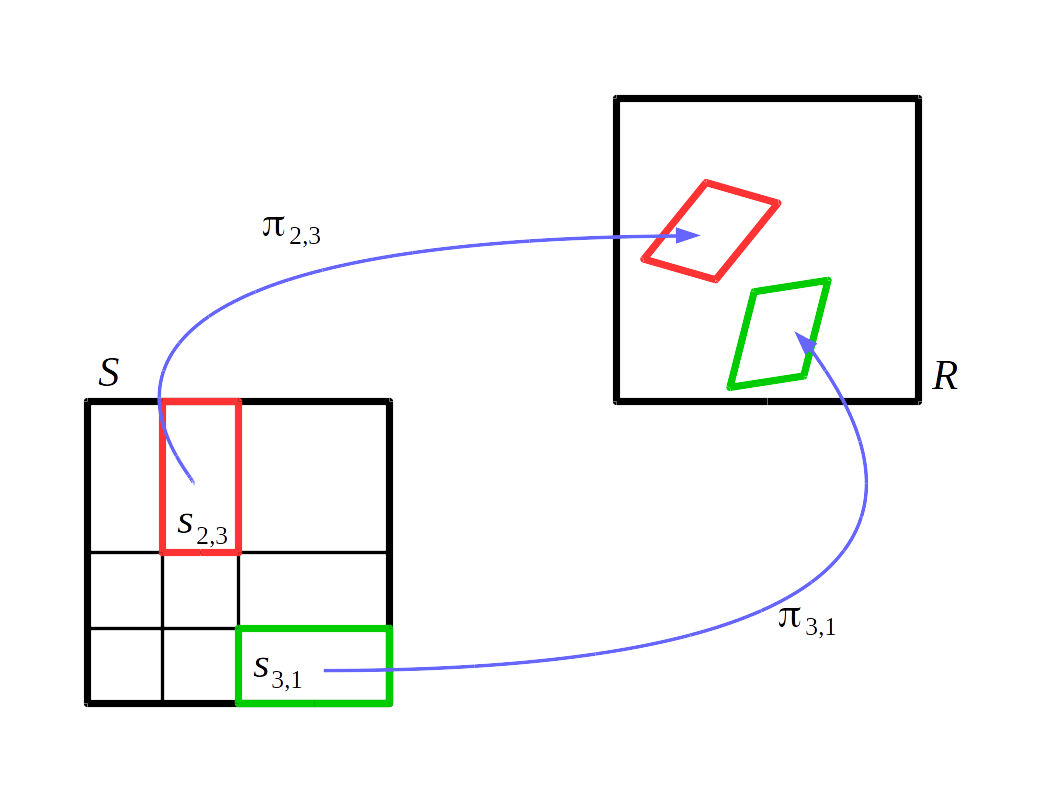
\includegraphics[trim = 0cm 2.2cm 0cm 2cm, clip, scale=0.25]{reachability.png}
  \caption{Mapping of tile $s_{2,3}$ to $R$ via pattern $\pi_{2,3}$,
and mapping of tile $s_{3,1}$ via  $\pi_{3,1}$.}
 \label{fig:reachability}
\end{figure}

%Actually, as mentioned above,
%we will focus on rectangles $S$  which  \emph{contain}  $R$
%(see Section \ref{ss:extension}).


\subsubsection{Parametric extension of tiling}\label{ss:extension}
In the following, we assume that the set $S$ we are looking for
is a \emph{parametric extension} of $R$, denoted by $R+(a,a)$,
which is defined in the following.

Suppose that $R=R_1\times R_2$ is given
as well as a tiling
${\cal R}={\cal R}_1\times {\cal R}_2=\{r_{i_1}\times r_{i_2}\}_{i_1\in I_1, i_2\in I_2}
=\{r_{i_1,i_2}\}_{i_1\in I_1, i_2\in I_2}$.
Then $R_1$ can be seen as a product of~$n_1$ closed intervals
of the form $[\ell,m]$. Consider a nonnegative real parameter~$a$.
Let $(R_1+a)$ denote the corresponding
product of $n_1$ intervals of the form
$[\ell-a,m+a]$.\footnote{Actually, we will consider in the examples
that $(R_1+a)$ is a product of intervals of
the form $[\ell-a,m]$ where the interval is extended only
at its \emph{lower} end, but the method is strictly identical.}
We define $(R_2+a)$ similarly.
Finally, we define $R+(a,a)$ as $(R_1+a)\times (R_2+a)$.

We now consider that $S$ is a (parametric) superset of~$R$
of the form $R+(a,a)$.
We define a tiling ${\cal S}={\cal S}_1\times{\cal S}_2$
of~$S$ of the form $\{s_{i_1}\times s_{i_2}\}_{i_1\in I_1,i_2\in I_2}$,
which is obtained from
%
${\cal R}={\cal R}_1\times{\cal R}_2=
\{r_{i_1}\times r_{i_2}\}_{i_1\in I_1,i_2\in I_2}$ by a simple extension,
as follows:
%
%Let ${\cal S}=\{s_{i_1,i_2}\}_{i_1\in I_1, i_2\in I_2}
%=\{s_{i_1}\times s_{i_2}\}_{i_1\in I_1, i_2\in I_2}$ be the finite rectangular 
%tiling of $S=R+(a,a)$ obtained from the tiling ${\cal R}$ as follows:
A~tile $r_{i_1}$ (resp.~$r_{i_2}$) of ${\cal R}_1$ (resp. ${\cal R}_2$)
in ``contact''
with $\partial R_1$ (resp.~$\partial R_2$)
is extended as a tile~$s_{i_1}$ (resp.~$s_{i_2}$)
in order to be in contact with~$\partial (R_1+a)$
(resp.~$\partial (R_2+a)$); 
a tile 
``interior'' to~$R_1$ (i.e.,~with no contact with~$\partial R_1$)
is kept unchanged, and coincides with~$s_{i_1}$,
and similarly for~$R_2$. 

We denote the resulting tiling ${\cal S}$ by ${\cal R}+(a,a)$.
We~also denote~$s_{i_1}$ (resp.~$s_{i_2}$)
by~$r_{i_1}+a$ (resp.~$r_{i_2}+a$), even if 
$r_{i_1}$ (resp.~$r_{i_2}$) is ``interior'' to~$R_1$
(resp.~$R_2$).
Likewise, we denote~$s_{i,j}$ by~$r_{i,j}+(a,a)$.
%
Note that a tiling of~$R$ of index set $I_1\times I_2$
induces a tiling of $R+(a,a)$ with the same index set
$I_1\times I_2$, hence the same number of tiles as~$R$, for any $a\geq 0$.
This is illustrated in Figure~\ref{fig:tiling2},
where the tiling of~$R$ is represented with black continuous lines,
and the extended tiling of $R+(a,a)$ with red dashed lines.

\begin{figure}[!h]
  \centering
 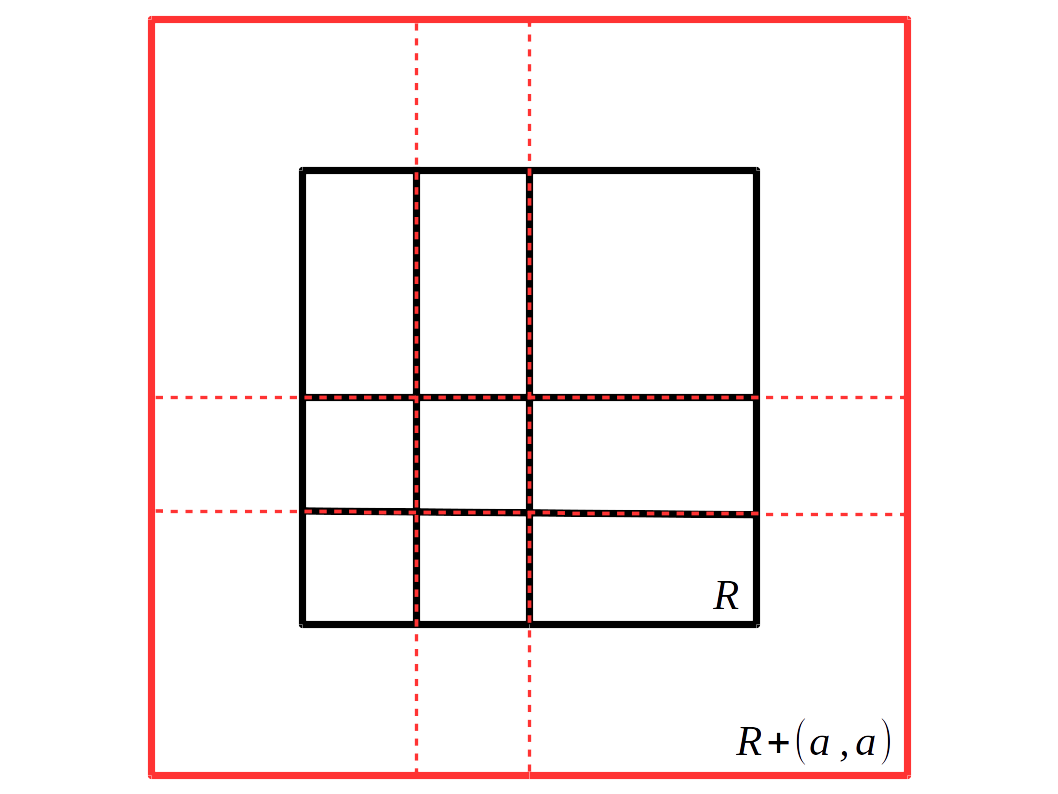
\includegraphics[trim = 0cm 0.3cm 0cm 0.3cm, clip, scale=0.18]{tiling_R.png}
  \caption{Tiling of $R+(a,a)$ induced by tiling ${\cal R}$ of $R$.}
 \label{fig:tiling2}
\end{figure}

\subsubsection{Generate-and-test tilings}\label{ss:gen}
By replacing $S$ with $R+(a,a)$ in the notions defined in
Section~\ref{ss:cent0} %and \ref{ss:dist0},
the problem of macro-step control synthesis can now be reformulated as:
``\emph{find a tiling ${\cal R}$ of~$R$ 
that induces a macro-step 
control of $R+(a,a)$  towards~$R$,  for some $a\geq 0$ (as big as possible)}''.

% besides,
%if we find such ${\cal R}$,
%we want to compute the \emph{maximum} value of $a$
%for which the induced control exists.

This problem can be solved by a simple ``generate-and-test''
procedure: we \emph{generate} a candidate tiling, and then 
\emph{test} if it satisfies the control property (the control test
procedure is explained in Section~\ref{ss:macro_cent}); if the test
fails, we~generate another candidate, and so on iteratively.

In practice, the generation of a candidate~${\cal R}$ is performed
by starting from the trivial tiling (made of one tile equal to~$R$), and
using successive \emph{bisections} of~$R$ until, either the control
test succeeds (``success''), or the depth of bisection of the new
candidate is greater than a given upper bound~$D$ (``failure'').  See
details in~\cite{fribourg2014finite}.%\fbox{+ ref previous papers}

%%%%%  Copie de l'annexe 1

%\fbox{Copie de l'annexe. A reduire un peu...}
\subsubsection{Tiling refinement}\label{ss:refinement}
Let us now explain how we find a tiling ${\cal R}$ of~$R$
such that $\Pi_{i_1,i_2}\neq \emptyset$.
We~focus on the centralized case, but the distributed case is similar.
We~start from the trivial tiling ${\cal R}^0=\{R\}$, which only contains
tile~$R$. If $f(R,\pi)\subseteq R$ for some $\pi\in \Pi^{\leq K}$,
then ${\cal R}^0$ is the desired tiling. Otherwise,
we~refine ${\cal R}^0$ by \emph{bisection}, which gives
a tiling ${\cal R}^1$ of the form $\{r_{(i,1),(j,2)}\}_{1\leq i,j\leq n}$.
If, for all $1\leq i,j\leq n$ there exists some $\pi\in \Pi^{\leq K}$ such that
$f(r_{(i,1),(j,2)},u)\subseteq R$, then ${\cal R}^1$ is the desired tiling.
Otherwise, there exist some ``bad'' tiles of the form $r_{(i,1),(j,2)}$
with $1\leq i,j\leq n$ such that $\forall \pi\in \Pi^{\leq K}\ f(r_{(i,1),(j,2)},\pi)\not\subseteq R$;
we then transform ${\cal R}^1$ into ${\cal R}^2$ by bisecting
all those bad tiles. By iterating this procedure, 
we produce tilings ${\cal R}^1, {\cal R}^2,\cdots, {\cal R}^d$, until
either no bad tiles remain in ${\cal R}^d$ (\emph{success}), 
or the bisection depth~$d$ is greater than
the given upper bound~$D$ (\emph{failure}).
%The treatment of the distributed control is similar.



\subsubsection{Iterated macro-step control synthesis}\label{ss:iteration}
Suppose that we are given an objective rectangle $R=R_1\times R_2$.
If the one-step control synthesis described in
Section~\ref{ss:refinement} succeeds, then there is a nonnegative real
$a^{(1)}=A$ and a tiling~${\cal R}$ of~$R$ that induces a control
steering all the points of $R^{(1)}=R+(a^{(1)},a^{(1)})$ to~$R$ in one
step.  Now the macro-step control synthesis can be reapplied
to~$R^{(1)}$.  If~it succeeds again, then it produces a tiling~${\cal
  R}^{(1)}$ of~$R^{(1)}$ which induces a control that steers
$R^{(2)}=R^{(1)}+(a^{(2)},a^{(2)})$ to~$R^{(1)}$ for some $a^{(2)}\geq
0$.
%in one step.
The iterated application
of macro-step control synthesis outputs a sequence of 
tilings~${\cal R}^{(i)}$,
each of which induces a control that steers 
$R^{(i+1)}=R+(\Sigma_{j=1}^{i+1}a^{(j)},\Sigma_{j=1}^{i+1}a^{(j)})$ 
to~$R^{(i)}$.
%, for some $a^{(j)}\geq 0$ ($1\leq j\leq i+1$).
In~the~end, this~synthesizes a control that steers~$R^{(i+1)}$
to~$R$ in at most $i+1$ macro-steps ($i\geq 0$),
using an increasing sequence of 
nested rectangles around~$R$.
This is illustrated in Figure \ref{fig:iteration}, for $i=1$.


The iteration process halts
at some step, say~$m$, when the last
macro-step control synthesis fails because
the maximum bisection depth~$D$ is reached while ``bad'' tiles still remain
(see~Section~\ref{ss:refinement}). We also stop
the process when the last macro-step control synthesis outputs
a real~$a^{(m)}$ which
is smaller than a given bound: this is because the 
sequence of controllable rectangles around $R$ seems to
approach a limit.


\begin{figure}[t]
  \centering
% 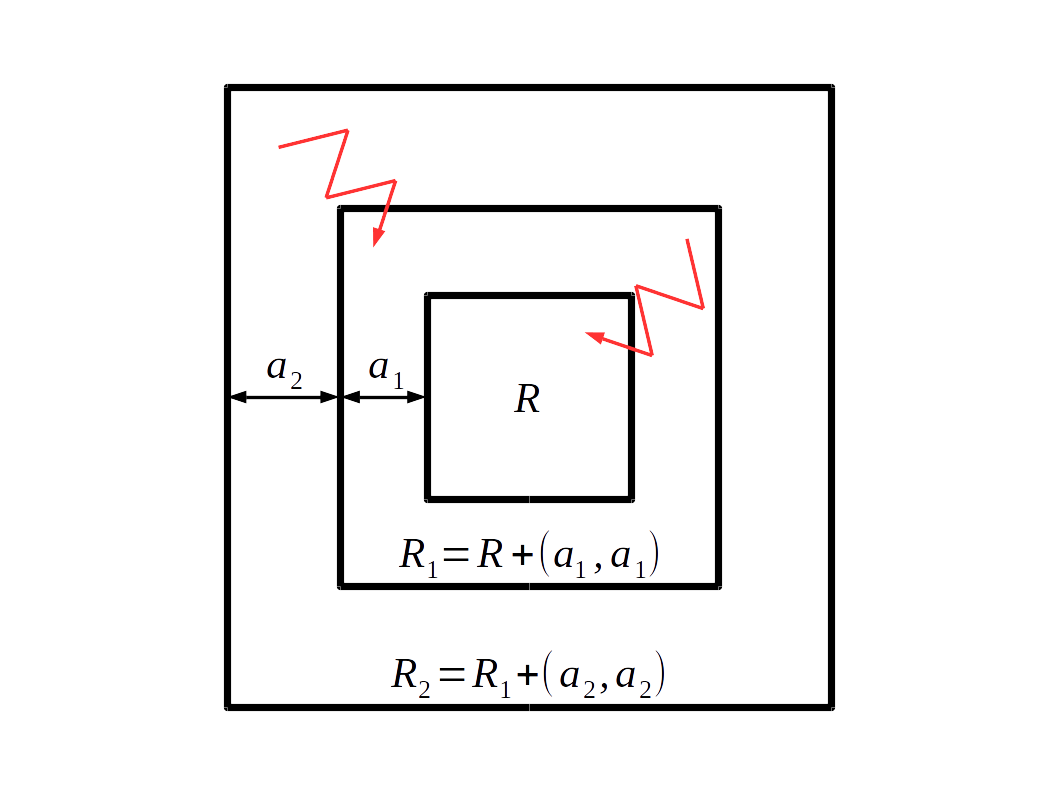
\includegraphics[scale=0.3]{iterated_reachability.png}
 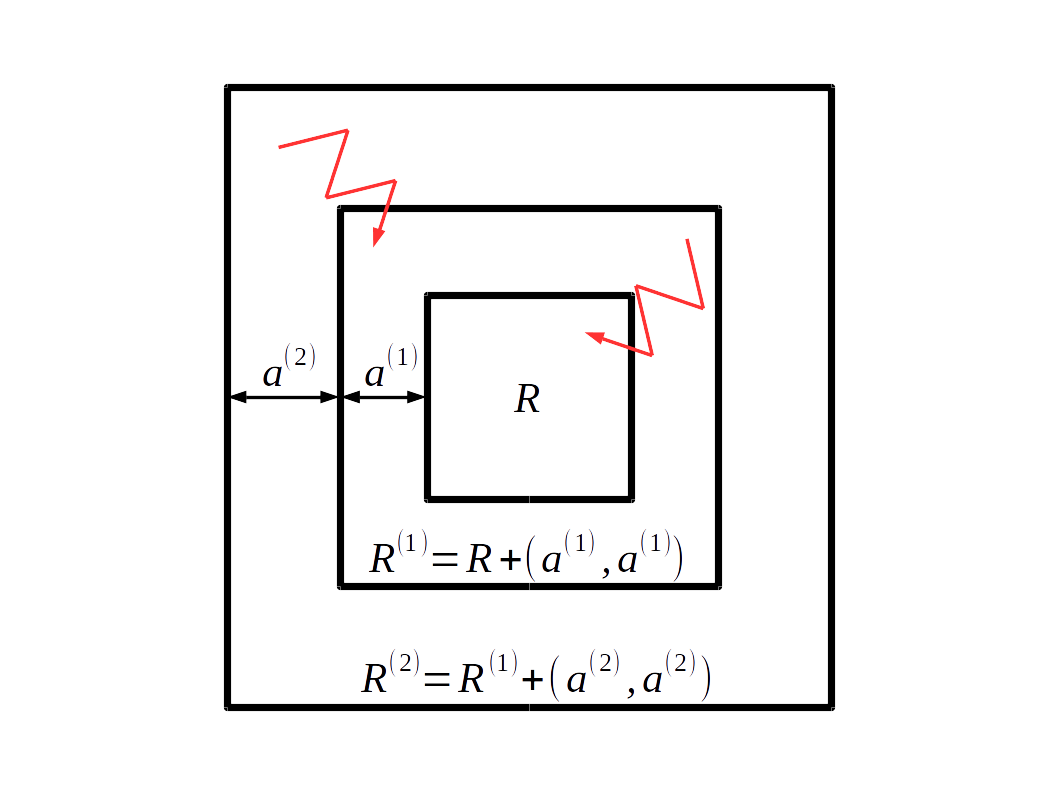
\includegraphics[trim = 0cm 1cm 0cm 1cm, clip, scale=0.25]{tiling_R_iterated.png}
  \caption{Iterated control of $R^{(1)}=R+(a^{(1)},a^{(1)})$ towards $R$,
and $R^{(2)}=R^{(1)}+(a^{(2)},a^{(2)})$ towards $R^{(1)}$.}
 \label{fig:iteration}
\end{figure}


%%%%% fin de l'annexe A1


%\emph{Remark 1.}
\begin{remark}\label{rk1}
Note that, if the generate-and-test process stops with ``success'' for a tiling
${\cal R}$, then the tiling
${\cal R}_{D,uniform}$ also solves the problem,
where ${\cal R}_{D,uniform}$
is the ``finest'' tiling obtained 
by bisecting $D$ times all the $n$ components of $R$.
Since ${\cal R}_{D,uniform}$ has exactly $2^{nD}$ tiles, 
it is in general impractical to perform directly the control test on it.
From a theoretical point of view however, 
it is convenient to suppose that ${\cal R}={\cal R}_{D,uniform}$ 
for reducing the \emph{worst case time complexity }
of the control synthesis procedure to the complexity 
of the control test part only
(see~Section~\ref{ss:macro_cent}).
\end{remark}


\subsection{Centralized control}\label{sec:one-step}
%We consider here 
%that we are given a tiling ${\cal R}$ of $R$
%of the form $\{r_{i_1,i_2}\}_{i_1\in I_1,i_2\in I_2}$.

\subsubsection{Tiling test procedure}\label{ss:macro_cent}

As seen in~Section \ref{ss:extension},
the \emph{(macro-step) 
control synthesis problem with horizon~K} 
consists in finding 
$a\geq 0$ (as big as possible), 
and a tiling ${{\cal R}=\{r_{i_1,i_2}\}_{i_1\in I_1, i_2\in I_2}}$ of~$R$
such that,
%
for each ${(i_1,i_2)\in I_1\times I_2}$,
there exists some~${\pi\in \Pi^{\leq K}}$ 
with
\begin{eqnarray}
f(r_{i_1,i_2}+(a,a),\pi)\subseteq R.
\label{a}
\end{eqnarray}
%
It is easy to see that if~\eqref{a} holds for some $a\geq 0$, then it
also holds for all $a'\leq a$.  In~order to \emph{test} if a tiling
candidate ${\cal R}=\{r_{i_1,i_2}\}_{i_1\in I_1,i_2\in I_2}$ of~$R$
satisfies the desired property, we~define, for each ${(i_1,i_2)\in
I_1\times I_2}$:
\begin{eqnarray}
\Pi_{i_1,i_2}^{\leq K}=\{\pi\in \Pi^{\leq K}\ |\ f(r_{i_1,i_2},\pi)\subseteq R\}.
%\label{a}
\end{eqnarray}
%
%$a_{i_1,i_2}$ by:
Suppose that $\Pi_{i_1,i_2}^{\leq K}\neq\emptyset$. Then we know that
Formula (\ref{a}) is satisfied for $a=0$. In~order to find~$a$ ``as
large as possible'', we~look for the existence of a pattern~$\pi$
such that Formula~\eqref{a} holds also for $a=\frac{|R|}{100}$ and
$a=\frac{|R|}{10}$, where $|R|$ denotes the length of the smallest
side of rectangle~$R$.  Numerous variants of such tests are of course
possible, but such a simple test works well in practice, and we keep
it here for the sake of simplicity.  When $\Pi_{i_1,i_2}^{\leq
  K}\neq\emptyset$, we thus define:
\begin{xalignat*}1
  a_{i_1,i_2} &=
  \max\{a\in\{0,\frac{|R|}{100},\frac{|R|}{10}\}\ |\ \exists \pi\in\Pi^{\leq K}\ 
  f(r_{i_1,i_2}+(a,a),\pi) \subseteq R\}.
 % \\
%  \pi_{i_1,i_2} &=
%%  \mathop{\textrm{argmax}}_{\pi\in\Pi_{i_1,i_2}^{\leq K}}\max\{a\geq 0\mid f(r_{i_1,i_2}+(a,a),\pi)
 %   \subseteq R\}
%    \\
\end{xalignat*}
Suppose that, for all $(i_1,i_2)\in I_1\times I_2$:
$\Pi_{i_1,i_2}^{\leq K}\neq\emptyset$, and
let $A=\min_{(i_1,i_2)\in I_1\times I_2}\{a_{i_1,i_2}\}$.
%
It is easy to see that,
for all $(i_1,i_2)\in I_1\times I_2$, there exists a pattern,
denoted by~$\pi_{i_1,i_2}$, such that:
%
$f(r_{i_1,i_2}+(A,A),\pi_{i_1,i_2}) \subseteq R.$
%




\begin{proposition}
%Let $W=\{W_{i_1}\times W_{i_2}\}_{(i_1,i_2)\in I_1\times I_2}$ be a 
%finite rectangular tiling of R.
%
%Suppose there exists a tiling 
%${\cal R}^0=\{r^0_{i,j}\}_{i\in I_1^0, j\in I_2^0}$
%of $R$ such that:
%$\forall (i,j)\in I_1^0\times I_2^0\ %\exists a\geq 0, 
%\exists \pi\in \Pi^{\leq K}\ 
%f((W_{i_1}+a)\times (W_{i_2}+a),\pi)\subseteq R,$$
%f(r_{i,j},\pi)\subseteq R$.
Suppose that there exists a tiling 
${\cal R}=\{r_{i_1,i_2}\}_{i_1\in I_1, i_2\in I_2}$ of $R$ such that:
%
$$\forall (i_1,i_2)\in I_1\times I_2\ \ \Pi_{i_1,i_2}^{\leq K}\neq \emptyset.$$
%
Then ${\cal R}$ induces
a macro-step control
of horizon $K$ of $R+(A,A)$ towards $R$ with:
%such that, for all $(i_1,i_2)\in I_{1}\times I_2$:
%
$$\forall (i_1,i_2)\in I_1\times I_2:\ 
\ \ f(r_{i_1,i_2}+(A,A),\pi_{i_1,i_2})\subseteq  R$$
%
where $A$ and $\pi_{i_1,i_2}$ are defined as above.
\end{proposition}



For each tile $r_{i_1,i_2}$ of $R$ and each $\pi\in\Pi^{\leq K}$, the
test of inclusion ${f(r_{i_1,i_2},\pi)\subseteq R}$ can be achieved in
time polynomial in~$n$ when $f$ is affine.
%
Hence the test $\Pi_{i_1,i_2}^{\leq K}\neq\emptyset$
can be done in $O(N^K \cdot n^{\alpha})$  
since $\Pi^{\leq K}$ contains $O(N^K)$ elements.
%
%The computation of $\max\{a\geq 0\ | f(r_{i_1,i_2}+(a,a),\pi)\subseteq R\}$
%can be done by \emph{linear programming} in time polynomial in $n$, 
%the dimension of the state space.
%
The computation time of $\{a_{i_1,i_2}\}_{i_1\in I,i_2\in I_2}$, $\pi_{i_1,i_2}$,
and $A$ is thus in $O(N^K \cdot 2^{nD})$, where $D$ is the maximal 
bisection depth.
Hence the complexity of testing
a candidate tiling~${\cal R}$ is in $O(N^K \cdot 2^{nD})$.
By~Remark~\ref{rk1} above, the running time of the 
control synthesis by the generate-and-test procedure is also in 
$O(N^K \cdot 2^{nD})$.
%
%We then have:



Once a candidate tiling ${\cal R}$ satisfying the control test
property is found, the generate-and-test procedure ends with
\emph{success} (see~Section \ref{ss:gen}), and a set
$S=R+(a^{(1)},a^{(1)})$ with $a^{(1)}=A$ has been found.  One can then
\emph{iterate} the ``generate-and-test'' procedure in order to
construct an increasing sequence of nested rectangles of the form
$R+(a^{(1)},a^{(1)})$, $R+(a^{(1)}+a^{(2)},a^{(1)}+a^{(2)})$, $\dots$,
which can all be driven to~$R$. The~process ends at the first step $i\geq 1$ 
for which $a^{(i)}=0$ (no~proper extension of the current
rectangle has been found).
%Appendix~\ref{ss:iteration}.




\begin{example}
\label{ex:ex2}
Consider the specification of a two-room apartment given in Example
\ref{ex:spec}. Set $R=[18.5,22]\times[18.5,22]$.
Let $D=1$ (the depth of bisection is at most 1),
and $K=4$ (the maximum length of patterns is~4).
We look for a centralized controller which will steer
the rectangle $S=[18.5-a,22]\times [18.5-a,22]$
to~$R$ with $a$ as large as possible, and stay in~$R$ indefinitely.
Using our implementation, the computation of the control synthesis
takes 4.14s of CPU time.

The method iterates successfully 15 times the macro-step control synthesis procedure.
We find $S=R+(a,a)$ with $a=53.5$, i.e. $S=[-35,22]\times[-35,22]$.
This means that any element of $S$ can be driven to $R$ within 15 macro-steps
of length (at most) 4, i.e., within $15\times 4=60$
units of time. 
Since each unit of time is of duration
$\tau=5$s, any trajectory starting from $S$ reaches $R$ within $60\times 5=300$s.
Once the trajectory $x(t)$ is in $R$, it returns in $R$
every macro-step of length (at most) 4, i.e., every $4\times 5=20$s.

These results are consistent with the simulation
given in Figure \ref{fig:simu_centralized} for the time evolution
of $(T_1,T_2)$ starting from $(12,12)$.
Simulations of the control, starting from $(T_1,T_2)=(12,12)$,
$(T_1,T_2)=(12,19)$ and $(T_1,T_2)=(22,12)$
are also given in the state space plane
in Figure \ref{fig:simu_centralized}.
\begin{figure}[t]
  \centering
%  \begin{tabular}{cc}
 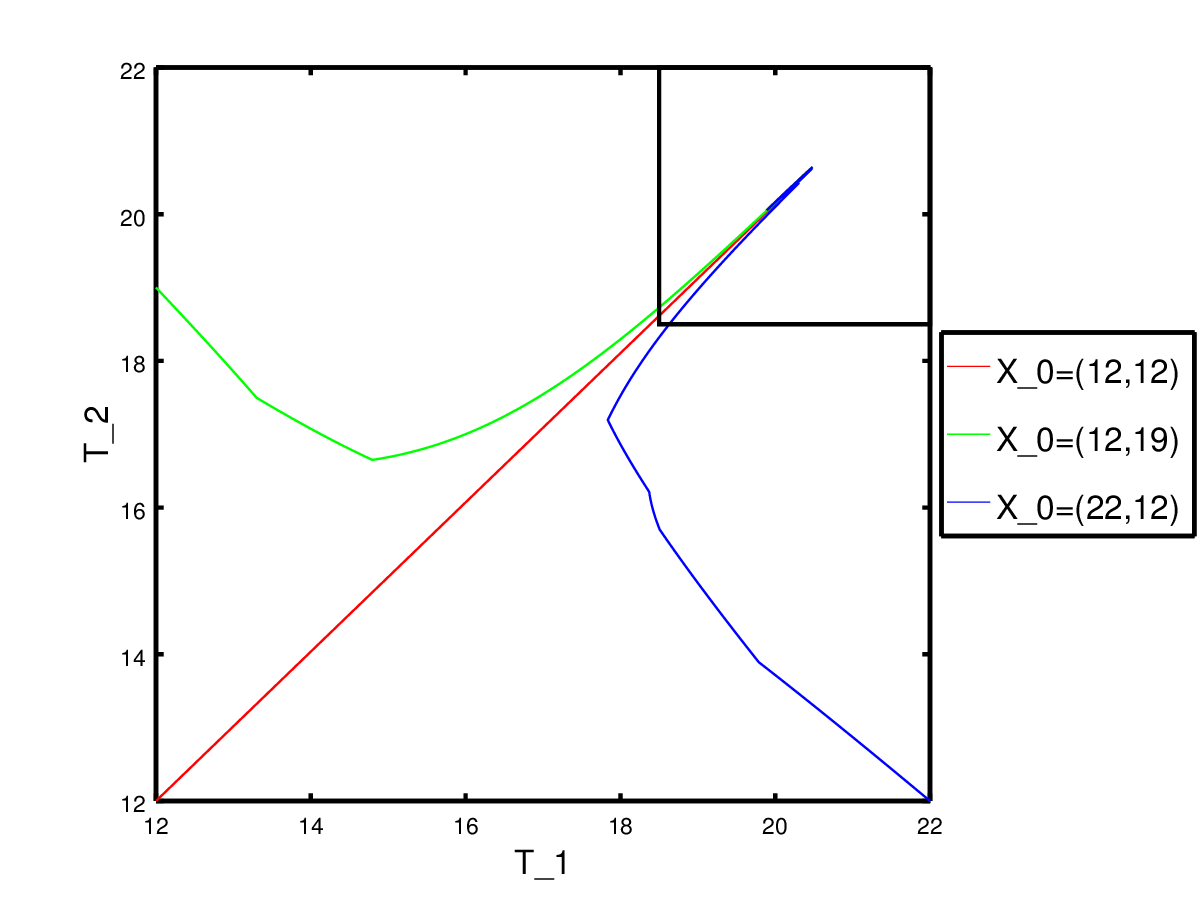
\includegraphics[trim = 0cm 0.3cm 0cm 1cm, clip, width=0.4\textwidth]{simu_2rooms_reach.png} 
% &
\qquad
 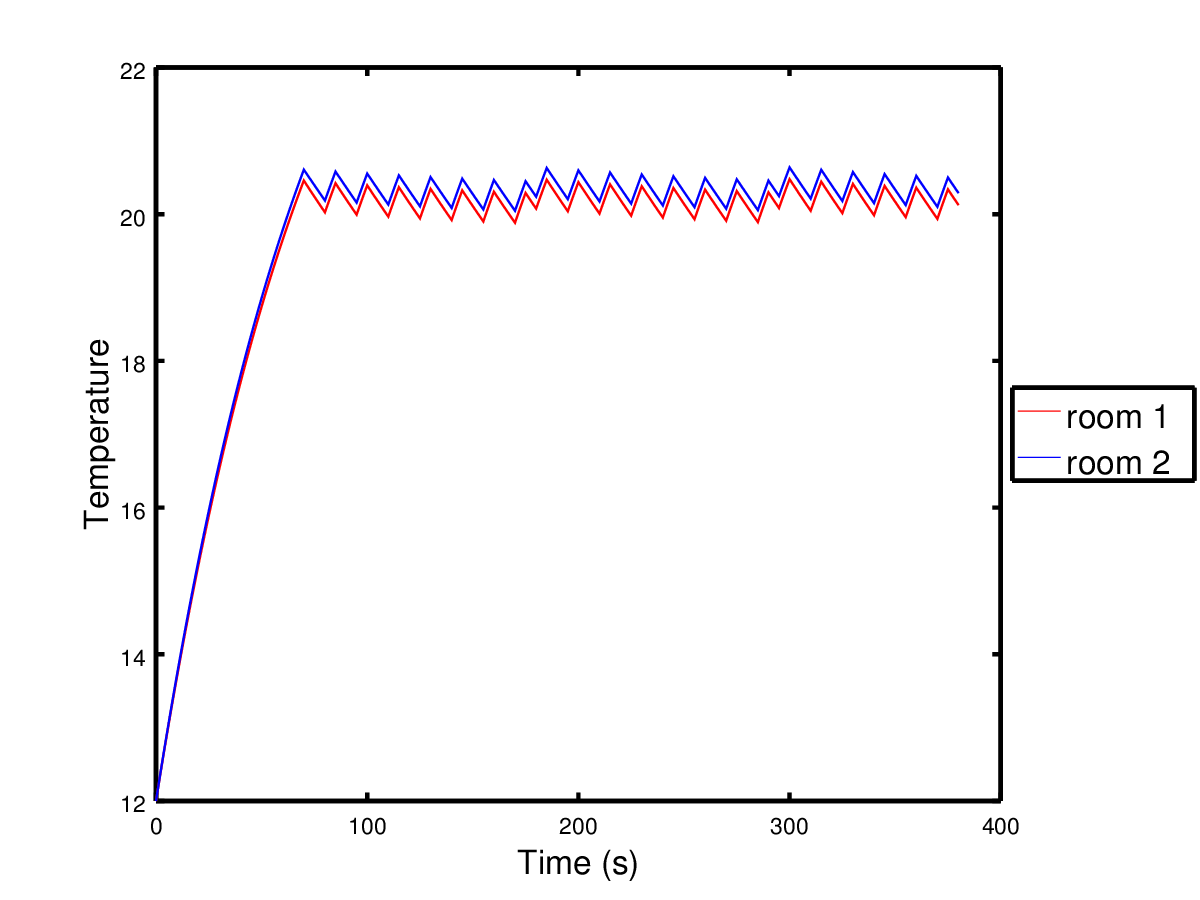
\includegraphics[trim = 0cm 0.3cm 0cm 1cm, clip, width=0.4\textwidth]{simu_centralized_time.png}
%  \end{tabular}

  \caption{Simulations of the centralized reachability controller for
    three different initial conditions plotted in the state space
    plane~(left); simulation of the centralized reachability
    controller for the initial condition $(12,12)$ plotted within
    time~(right).}
  \label{fig:simu_centralized}
\end{figure}
% \begin{figure}[!h]
%   \centering
% 
%   \caption{.}
%  \label{fig:simu_centralized_time}
% \end{figure}
% 
% 
 \end{example}


\subsubsection{Stability as a special case of reachability}\label{ss:special}
Instead of looking for a set of the form $S=R+(a,a)$ from
which $R$ is reachable via a macro-step,
let us consider the particular case where~${S=R}$ (i.e.,~$a=0$).


The problem now consists in constructing a tiling ${\cal
  R}=\{r_{i_1,i_2}\}_{i_1\in I_1, i_2\in I_2}$ of~$R$ such that, for
all $(i_1,i_2)\in I_1\times I_2$, there exists a pattern
$\pi_{i_1,i_2}\in \Pi^{\leq K}$ with ${f(r_{i_1,i_2},
  \pi_{i_1,i_2})\subseteq R}$.  If~such a tiling~${\cal R}$ exists,
then\footnote{If
  $x(t)\in R$, then $x(t)\in r_{i,j}$ for some $(i,j)\in I_1\times
  I_2$, hence $x(t+k)=f(x,\pi_{i,j})\in R$ for some $k\leq K$.}
$x(t)\in R$ implies $x(t+k)\in R$ for some ${k\leq K}$.
Actually, we can slightly modify the procedure in order to
additionally impose that for some $\varepsilon>0$, it~holds $x(t+k')\in
R+(\varepsilon,\varepsilon)$ for any $k'=1,\dots,k-1$
(see~Section~\ref{ss:macro_dist}).  It~follows that $R$ is ``stable''
(with tolerance~$\varepsilon$) under the control induced by~${\cal
  R}$.
%A similar result holds in the distributed context.
%
We can thus treat the stability control of~$R$ 
as a special case  of reachability control.
%with $S=R$ (i.e., $a=0$).





%\section{Macro-steps and Patterns}

\subsection{Distributed control}\label{sec:distr}
\subsubsection{Background}

In the distributed context,
given a set $R=R_1\times R_2$,
the \emph{(macro-step) distributed 
control synthesis problem with horizon~K} 
consists in finding $a\geq 0$, and
a tiling ${\cal R}_1=\{r_{i_1}\}_{i_1\in I_1}$ of $R_1$
which induces a (macro-step) control
on $R_1+a$, a 
tiling ${\cal R}_2=\{r_{i_2}\}_{i_2\in I_2}$
which induces a (macro-step) control on $R_2+a$.

More precisely, we seek tilings ${\cal R}_1$ and ${\cal R}_2$ such that:
%a set $S=S_1\times S_2$ containing $R$ and a tiling
%${\cal  S}_1\times {\cal  S}_2=\{s_{i_1}\}_{i\in I_1}\times\{s_{i_2}\}_{i\in I_2}$ of $S$ such that,
there exists $\ell\in{\mathbb N}$ such
that, for each $i_1\in I_1$ there exists a pattern
$\pi_1$ of $\ell$ modes in $U_1$,
and for each $i_2\in I_2$, 
a pattern $\pi_{2}$ 
of $\ell$ modes in $U_2$ such that:
%
\[
f((r_{i_1}+a)\times (R_2+a),(\pi_1,\pi_2))_{|1}\subseteq R_1 \ \wedge\ 
f((R_1+a)\times (r_{i_2}+a),(\pi_1,\pi_2))_{|2}\subseteq R_2.
\]


In order to synthesize a \emph{distributed} strategy where the control
pattern $\pi_1$ is determined only by $i_1$ (regardless of the value
of $i_2$), and the control pattern $\pi_2$ only by $i_2$ (regardless
of the value of $i_1$), we now define an \emph{over-approximation}
$X_{i_1}(a,\pi_1)$ for
$f((r_{i_1}+a)\times(R_2+a),(\pi_1,\pi_2))_{|1}$, and an
\emph{over-approximation} $X_{i_2}(a,\pi_2)$ for $f((R_1+a)\times
(r_{i_2}+a),(\pi_1,\pi_2))_{|2}$.  The correctness of these
over-approximations relies on the existence of a fixed positive value
for parameter $\varepsilon$.
% parameter 
% $\varepsilon$ of fixed positive real value.
Intuitively, $\varepsilon$ represents the width of
the additional margin (around $R+(a,a)$)
within which all the intermediate states lie when
a macro-step is applied to a point of $R+(a,a)$. 

\subsubsection{Tiling test procedure}\label{ss:macro_dist}

Let $\pi_1^k$ (resp.$\pi_2^k$) denote the prefix of length $k$
of $\pi_1$ (resp.$\pi_2$), and $\pi_1(k)$ (resp. $\pi_2(k)$)
the $k$-th element of pattern $\pi_1$ (resp. $\pi_2$).
\begin{definition}\label{def:1}
Consider an element $r_{i_1}$ (resp. $r_{i_2}$) of a tiling ${\cal
  R}_1$ (resp.~${\cal R}_2$) of~$R_1$ (resp.~$R_2$), and a~pattern
${\pi_1\in\Pi_1^{\leq K}}$ (resp.~${\pi_2\in\Pi_2^{\leq K}}$) of
length~$\ell_1$ (resp.~$\ell_2$).  The \emph{approximate
  first-component (resp. second-component) sequence}
$\{X^k_{i_1}(a,\pi_1)\}_{0\leq k\leq \ell_1}$
(resp. $\{X^k_{i_2}(a,\pi_2)\}_{0\leq k\leq \ell_2}$) is defined as
follows:
\begin{itemize}
\item $X^0_{i_1}(a,\pi_1)=r_{i_1}+a$
  (resp. $X^0_{i_2}(a,\pi_2)=r_{i_2}+a$)
  and 
\item $X^{k}_{i_1}(a,\pi_1)=f_1(X^{k-1}_{i_1}(a,\pi_1),R_2+a+\varepsilon,\pi_1(k))$ for $1\leq k\leq \ell_1$
  (resp. $X^{k}_{i_2}(a,\pi_2)=f_2(R_1+a+\varepsilon,X^{k-1}_{i_2}(a,\pi_2),\pi_2(k))$
for $1\leq k\leq\ell_2$).
%
\end{itemize}
%% (resp. 
%% \begin{itemize}
%% \item $X^0_{i_2}(a,\pi_2)=r_{i_2}+a$ and 
%% \item $X^{k}_{i_2}(a,\pi_2)=f_2(R_1+a+\varepsilon,X^{k-1}_{i_2}(a,\pi_2),\pi_2(k))$
%% for $1\leq k\leq\ell_2$).
%% \end{itemize}
%
\end{definition}
%


We define the property
%
$\Prop_1(a,i_1,\pi_1)$ of $\{X^k_{i_1}(a,\pi_1)\}_{0\leq k\leq \ell_1}$ by:
%$\{X^{k}_1\}_{0\leq k\leq \ell_1}$ such that:
%\begin{itemize}
%\item
\begin{center}
$X^{k}_{i_1}(a,\pi_1)\subseteq R_1+a+\varepsilon$ for $1\leq k\leq \ell_{1}-1$, and
%\item
$X_{i_1}^{\ell_{1}}(a,\pi_1)\subseteq R_1$.
\end{center}
%\end{itemize}
%
Likewise, we define the property
%
$\Prop_2(a,i_2,\pi_2)$ of $\{X^k_{i_2}(a,\pi_2)\}_{0\leq k\leq \ell_2}$ by:
%$\{X^{k}_1\}_{0\leq k\leq \ell_1}$ such that:
%\begin{itemize}
%\item
\begin{center}
$X^{k}_{i_2}(a,\pi_2)\subseteq R_2+a+\varepsilon$ for $1\leq k\leq \ell_{2}-1$, and
  %\item
$X_{i_2}^{\ell_{2}}(a,\pi_2)\subseteq R_2$.
\end{center}
  %\end{itemize}
%
Figure \ref{fig:Q1} illustrates property $\Prop_1(a,i_1,\pi_1)$
for $\pi_1=(u_1\cdot v_1)$,
$\ell_1=2$ and a given tile $r_{i_1}$ with $i_1 \in I_1$:
 $\Prop_1(a,i_1,\pi_1)$ is satisfied because
$X_1^1(a,\pi_1)\subseteq R_1+a+\varepsilon$
and $X_1^2(a,\pi_1)\subseteq R_1$  are true.
% in the lower part, $\Prop_1(a,i_1,\pi_1)$
% is satisfied.



\begin{figure}[t]
  \centering
%  \begin{tabular}{cc}
 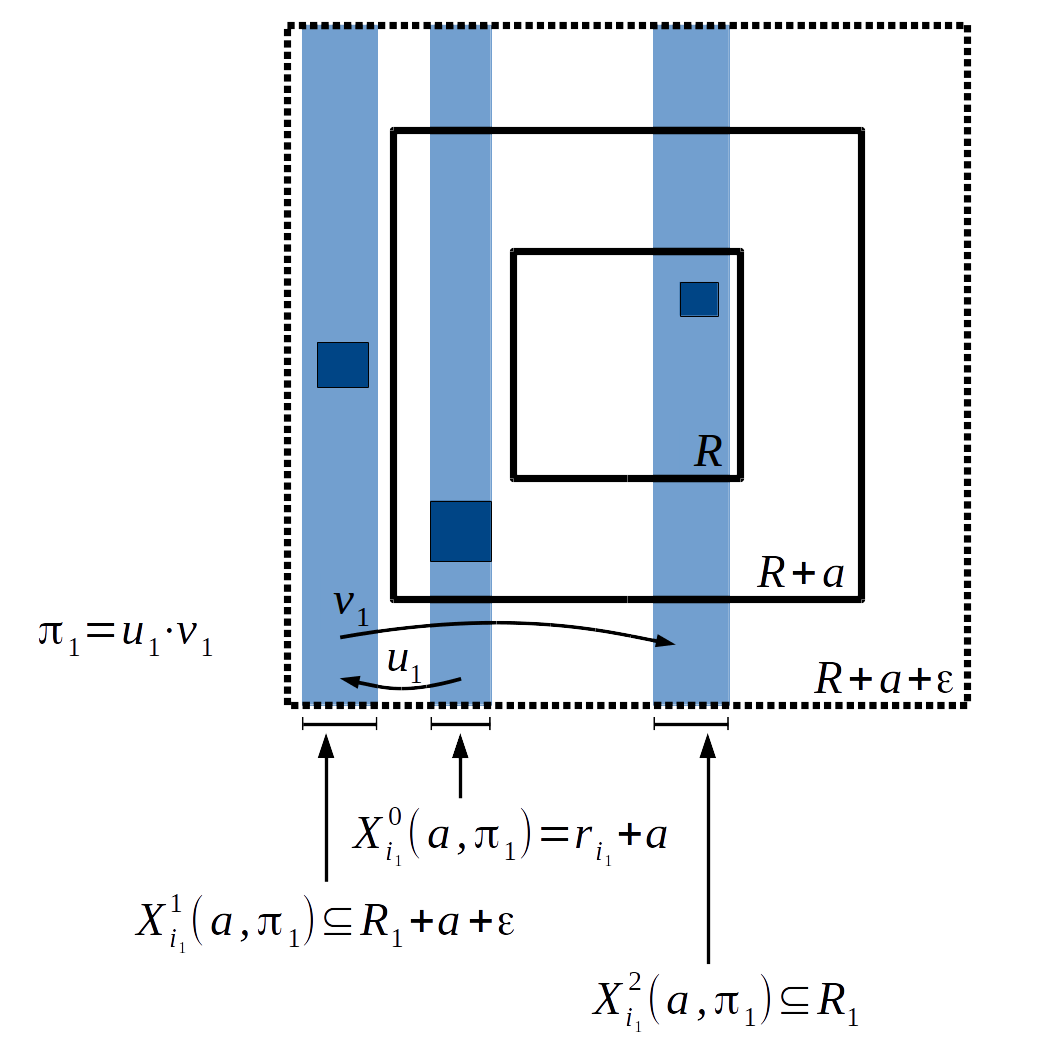
\includegraphics[trim = 0cm 0cm 0cm 0cm, clip, width=0.65\textwidth]{distributed_explanation1.png}
 % &
%  \qquad
%  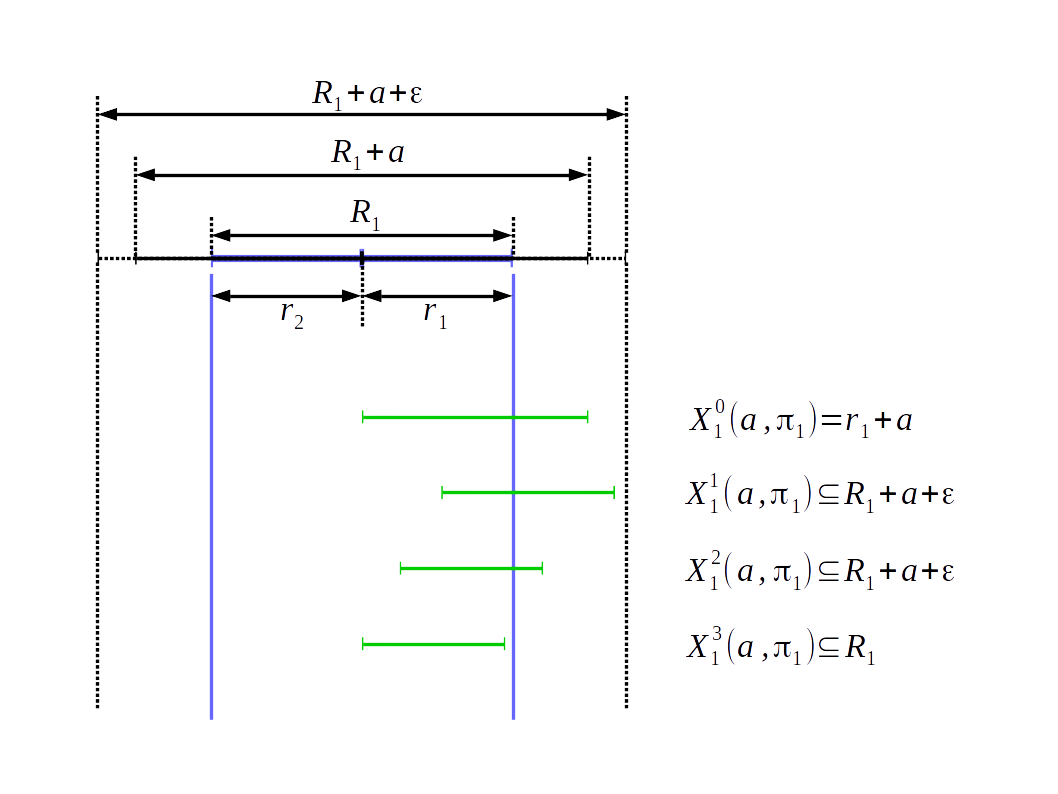
\includegraphics[trim = 2cm 1cm 2cm 2cm, clip, width=0.45\textwidth]{safety_true.png}
%  \end{tabular}

  \caption{Illustration of  $\Prop_1(a,i_1,\pi_1)$  with $i_1 \in I_1$,
$|\pi_1|=\ell_1=2$. The dark blue squares represent the centralized case, where both dimensions
are controlled. The pale blue ribbons represent the distributed case, where we control only
the first dimension, and over-approximate the behavior of the centralized case.}
 \label{fig:Q1}
\end{figure}

\medskip
%Given a tiling ${\cal R}_1=\{r_{i_1}\}_{i_1\in I_1}$  of $R_1$,
%we now define, for each $i_1\in I_1$:
%\[\Pi_{i_1}^{\ell_1}=\{\pi_1\in \Pi_1^{\ell_1}\ |\ 
%\Prop_1(0,i_1,\pi_1)\}.
%\]

Suppose now that there exist $\ell_1$ and $\ell_2$
($1\leq \ell_1,\ell_2\leq K$) such that:
\begin{description}
\item[$H1(\ell_1)$:] 
$\forall i_1\in I_1\  
\exists \pi_1\in \Pi_1^{\ell_1}\  
\Prop_1(0,i_1,\pi_1)$.
%\Pi_{i_1}^{\ell_1}\neq \emptyset$.

\item[$H2(\ell_2)$:] 
$\forall i_2\in I_2\  
\exists \pi_2\in \Pi_2^{\ell_2}\  
\Prop_1(0,i_1,\pi_2)$.
%  $\forall i_2\in I_2\ \Pi_{i_2}^{\ell_2}\neq \emptyset$.
\end{description}
Then we define:
\begin{xalignat*}1
a(\ell_1) & =  \max\{a\in\{0,\frac{|R|}{100},\frac{|R|}{10}\}\mid \forall i_1\in I_1\ \exists \pi_1\in \Pi_1^{\ell_1}\ \Prop_1(a,i_1,\pi_1)\}.
\end{xalignat*}
\begin{xalignat*}1
a(\ell_2) & =  \max\{a\in\{0,\frac{|R|}{100},\frac{|R|}{10}\}\mid \forall i_2\in I_2\ \exists \pi_2\in \Pi_2^{\ell_2}\ \Prop_2(a,i_2,\pi_2)\}.
\end{xalignat*}
Let
$A=\min\{a(\ell_1),a(\ell_2)\}$.
%
From $H1(\ell_1)$-$H2(\ell_2)$, it follows 
that, for all $i_1\in I_1$ there exists
a pattern of~$\Pi_1^{\ell_1}$, denoted by $\pi_{i_1}$, such that
$Prop_1(A,i_1,\pi_{i_1})$, and there exists
a pattern of~$\Pi_2^{\ell_2}$, denoted by $\pi_{i_2}$ such that
$Prop_2(A,i_2,\pi_{i_2})$.

\begin{remark}
  Given a tiling ${\cal R}={\cal R}_1\times{\cal R}_2$, $H1(\ell_1)$ means
  that the points of $R_1+A$ can be (macro-step) controlled to $R_1$
  using patterns which all have the \emph{same length} $\ell_1$; in other
  terms, all the macro-steps controlling $R_1+A$ contain the same
  number $\ell_1$ of elementary steps.  And symmetrically for $H2(\ell_2)$.
\end{remark}
\begin{remark}
  The selection of an appropriate value for~$\varepsilon$ is for the
  moment performed by hand, and is the result of a compromise: if
  $\varepsilon$ is too small, then $f_1(r_{i_1},R_2,\pi_1(1))\subseteq
  R_1+\varepsilon$ for no $\pi_1\in\Pi^{\ell_1}$; if $\varepsilon$ is
  too large, then
  $f_1(X_{i_1}^{\ell_1},R_2+\varepsilon,\pi_1(\ell_1))\subseteq R_1$
  for no $\pi_1\in\Pi^{\ell_1}$.
\end{remark}

%Given a tiling ${\cal R}={\cal R}_1\times{\cal R}_2$ of $R$
%and a real $\varepsilon>0$,
%the problem of existence and computation of
%$k_1$, $k_2$,
%$\{\pi_{i_1}^{k_1}\}_{i_1\in I_1}$,
%$\{\pi_{i_2}^{k_2}\}_{i_2\in I_2}$, and $A$
%can be solved by
%\emph{linear programming} since $f_1$ and $f_2$ are affine.
%
Using the same kinds of calculation as in the centralized case (see
Section~\ref{ss:macro_cent}), one can see that
finding $\ell_1,\ell_2$ such that $\Pi_{i_1}^{\ell_1}\neq \emptyset$
and $\Pi_{i_2}^{\ell_2}\neq \emptyset$,
%checking $H1(\ell_1)$-$H(\ell_2)$,
generating $A$ and $\{\pi_{i_1}\}_{i_1\in I_1}$,
and $\{\pi_{i_2}\}_{i_2\in I_2}$,
can be performed in time $O((\max(N_1,N_2))^K\cdot 2^{\max(n_1,n_2)D})$.
Hence the running time of the control test procedure is also in
$O((\max(N_1,N_2))^K\cdot 2^{\max(n_1,n_2)D})$.

\begin{lemma}\label{prop:lemma}
Consider a tiling ${\cal R}={\cal R}_1\times{\cal R}_2$ of the
form $\{r_{i_1}\times r_{i_2}\}_{(i_1,i_2)\in I_1\times I_2}$.
% Let $i_1\in I_1, i_2\in I_2$ and $a>0$.
%Let $a\geq 0$. 
Suppose that $H1(\ell_1)$ and $H2(\ell_2)$ hold for some
$\ell_1,\ell_2\leq K$.
%, which means that there exists $A\geq 0$ such that for all
%$i_1 \in I_1$, $\Prop_1(A,i_1,\pi_{1})$ holds for some $\pi_{1}\in
%\Pi_1^{\ell_1}$, and for all $i_2 \in I_2$, $\Prop_2(A,i_2,\pi_{2})$
%holds for some $\pi_{2}\in \Pi_2^{\ell_2}$. 
Then we have:

\begin{itemize}
\item in case $\ell_1\leq \ell_2$: for all $1\leq k\leq \ell_1$ and all $i_1\in I_1$,
\begin{xalignat*}1
  f((r_{i_1}+A) \times (R_2+A),(\pi_{i_1}^k,\pi_{i_2}^k))_{|1}
   & \subseteq X_{i_1}^k(A,\pi_{i_1}) \subseteq R_1+A+\varepsilon 
\\
f((R_1+A)\times(r_{i_2}+A),(\pi_{i_1}^k,\pi_{i_2}^k))_{|2}
&\subseteq X_{i_2}^k(A,\pi_{i_2})\subseteq R_2+A+\varepsilon
%\tag{for all $1\leq k\leq \ell_1$}
\\
f((r_{i_1}+A)\times( R_2+A),(\pi_{i_1}^{\ell_1},\pi_{i_2}^{\ell_1}))_{|1}
   &\subseteq X_{i_1}^{\ell_1}(A,\pi_{i_1})\subseteq R_1
\end{xalignat*}

\item in case $\ell_2 \leq \ell_1$: for all $1\leq k\leq \ell_2$ and all $i_2\in I_2$,
  \begin{xalignat*}1
    f((r_{i_1}+A)\times( R_2+A),(\pi_{i_1}^k,\pi_{i_2}^k))_{|1}
      &\subseteq X_{i_1}^k(A,\pi_{i_1})\subseteq R_1+A+\varepsilon
    \\
    f((R_1+A)\times(r_{i_2}+A),(\pi_{i_1}^k,\pi_{i_2}^k)){|_2}
    &\subseteq X_{i_2}^k(A,\pi_{i_2})\subseteq R_2+A+\varepsilon
    \\
%\hspace*{\fill}for all $1\leq k\leq \ell_2$, and
    f((R_1+A)\times(r_{i_2}+A),(\pi_{i_1}^{\ell_2},\pi_{i_2}^{\ell_2}))_{|2}
      &\subseteq X_{i_2}^{\ell_2}(A,\pi_{i_2})\subseteq R_2.
  \end{xalignat*}


\end{itemize}

\end{lemma}
%
%The proof is given in Appendix \ref{sec:proof}.
%\fbox{mettre la preuve ici ?}

\begin{proof}
Suppose $\ell_1 \leq \ell_2$, and
denote by $P_{i_1}^1(k)$ the property
\begin{equation*}
(f((r_{i_1}+A,R_2+A),(\pi_{i_1}^k,\pi_{i_2}^k)))_1 \subseteq X_{i_1}^k
 \label{eq:firstinc}
\end{equation*}
and by $P_{i_1}^2(k)$
\begin{equation*}
X_{i_1}^k \subseteq R_1 + A + \varepsilon
 \label{eq:secondinc}
\end{equation*}
and similarly for $P_{i_2}^1(k)$ and $P_{i_2}^2(k)$.

We show by induction on~$k$ the following property~$P(k)$:
\begin{equation*}
\forall i_1 \in I_1, \ P_{i_1}^1(k) \wedge  P_{i_1}^2(k) \quad \text{and} \quad \forall i_2 \in I_2, \ P_{i_2}^1(k) \wedge  P_{i_2}^2(k). 
\end{equation*}

Let us first consider the case $k = 1$.  Let us prove $\forall i_1 \in
I_1, \ P_{i_1}^1(k) \wedge P_{i_1}^2(k)$ (the~proof is similar for
$\forall i_2 \in I_2, \ P_{i_2}^1(k) \wedge P_{i_2}^2(k)$).  Let us
show that $(f((r_{i_1}+A,R_2+A),(\pi_{i_1}^k,\pi_{i_2}^k)))_1
\subseteq X_{i_1}^k$ and $X_{i_1}^k \subseteq R_1 + A + \varepsilon$.

For $k = 1$,
$\pi_{i_1}^k$ and $\pi_{i_2}^k$ are of the form $u_1$ and $u_2$. We have:
\begin{enumerate}
 \item $(f((r_{i_1}+A,R_2+A),(\pi_{i_1}^k,\pi_{i_2}^k)))_1 = f_1(r_{i_1} + a, R_2 + a, u_1)$
 \item $X_{i_1}^1 = f_1(X_{i_1}^0,R_2 + A + \varepsilon, u_1) = f_1(r_{i_1} + a ,R_2 + A + \varepsilon, u_1) $
\end{enumerate}

Hence $(f((r_{i_1}+A,R_2+A),(\pi_{i_1}^k,\pi_{i_2}^k)))_1 \subseteq X_{i_1}^k$ holds
for $k=1$. And $X_{i_1}^k \subseteq R_1 + A + \varepsilon$ because 
of $\Prop_1(A,i_1,\pi_{i_1})$. 




Let us now suppose that $k>1$ and that $P(k-1)$ holds. We~prove~$P(k)$.
Properties $P_{i_1}^2(k)$ and $P_{i_2}^2(k)$ are true for all $i_1,i_2$ because, 
by~construction, the sequence $X_{i_1}^k$ (resp. $X_{i_2}^k$)
satisfies $\Prop_1(a,i_1,\pi_{i_1})$ (resp. $\Prop_2(a,i_2,\pi_{i_2})$).
Let us prove $P_{i_1}^1(k)$ and $P_{i_2}^1(k)$:

\begin{xalignat*}1
  (f(r_{i_1} +A,R_2+A,(\pi_{i_1}^k,\pi_{i_2}^k)))_1 & = (f(f((r_{i_1}+A,R_2+A),(\pi_{i_1}^{k-1},\pi_{i_2}^{k-1})),\\
  \noalign{\hfill$(\pi_{i_1}{(k)},\pi_{i_2}{(k)})))_1$}
  & =  f_1(\lbrack f((r_{i_1}+A,R_2+A),(\pi_{i_1}^{k-1},\pi_{i_2}^{k-1})) \rbrack, \\
 \noalign{\hfill$\lbrack f((r_{i_1}+A,R_2+A),(\pi_{i_1}^{k-1},\pi_{i_2}^{k-1})) \rbrack
,\pi_{i_1}{(k)})$.} 
\end{xalignat*}
 
 Note that  the first argument of $f_1$ in the last expression satisfies
  $\lbrack f((r_{i_1}+A,R_2+A),(\pi_{i_1}^{k-1},\pi_{i_2}^{k-1}))\rbrack \subseteq X_{i_1}^k $
  by $P_{i_1}^1(k-1)$. Besides, the second argument
  satisfies $\lbrack f((r_{i_1}+A,R_2+A),(\pi_{i_1}^{k-1},\pi_{i_2}^{k-1})) \rbrack
  \subseteq \bigcup_{j_2 \in I_2}X_{j_2}^{k-1} \subseteq R_2 + A + \varepsilon$, because 
  \begin{enumerate}
   \item $r_{i_1} + A \subseteq R_{1}+A$
%    \item $R_2 + a = \bigcup_{j_2 \in I_2} r_{j_2}$
   \item $\bigcup_{j_2 \in I_2} X_{j_2}^{k-1} \subseteq R_2 + A + \varepsilon$ since $X_{j_2}^{k-1} \subseteq R_2 + A + \varepsilon$ \quad (by $P_{j_2}^2(k-1)$ which holds for all $j_2$)
   \item $\lbrack f((R_1 + A , r_{j_2} + A), (\pi_{i_1}^{k-1}, \pi_{i_2}^{k-1})) \rbrack 
  \subseteq X_{j_2}^{k-1}$ \quad (by $P_{j_2}^1(k-1)$).
  \end{enumerate}
  

%   $r_{i_1} + a \subseteq R_{1}+a$ and $R_2 + a = \bigcup_{j_2 \in I2} r_{j_2}$,
%   and $X_{i_2}^{k-1} \subseteq R_2 + A + \varepsilon$ (this is $P_{i_2}^2(k-1)$)
%   and $\lbrack f((R_1 + a , r_{j_2} + a), (\pi_{i_1}(k-1), \pi_{i_2}(k-1))) \rbrack
%   \subseteq X_{j_2}^{k-1}$.
 
 
 Hence 
 \begin{eqnarray*}
  f_1(\lbrack f((r_{i_1}+A,R_2+A),(\pi_{i_1}^{k-1},\pi_{i_2}^{k-1})) \rbrack,\lbrack f((r_{i_1}+A,R_2+A),(\pi_{i_1}^{k-1},\pi_{i_2}^{k-1})) \rbrack,\pi_{i_1}^{(k)} ) \\
  \subseteq f_1(X_{i_1}^{k-1},R_2 + A + \varepsilon,\pi_{i_1}(k)) = X_{i_1}^k
 \end{eqnarray*}

 
 We have thus proved $P_{i_1}^1(k)$:
 \begin{equation*}
 (f(r_{i_1} +A,R_2+A,(\pi_{i_1}^k,\pi_{i_2}^k)))_1 \subseteq X_{i_1}^k
\end{equation*}
This completes the proof of $\forall i_1 \in I_1,\  P_{i_1}^1(k) \wedge P_{i_1}^2(k)$
We prove $P_{i_2}^1(k) \wedge P_{i_2}^2(k)$ for all $i_2 \in I_2$ 
similarly, which concludes the proof of~$P(k)$.
%
The proof of
$(f((r_{i_1}+A,R_2+A),(\pi_{i_1}^{\ell_1},\pi_{i_2}^{\ell_1})))_1
\subseteq X_{i_1}^{\ell_1}(a,\pi_{i_1}) \subseteq R_1$ is similar.
% Note that 
% 
% , and we have
% $X_{i_1}^1 = f_1(X_{i_1}^0,R_2 + A + \varepsilon, u_1) = f_1(r_{i_1} + a ,R_2 + A + \varepsilon, u_1) $
% 
\end{proof}



At $t=0$, consider a point $x(0)=(x_1(0),x_2(0))$ of $R+(A,A)$,
and let us apply concurrently the strategy induced by ${\cal R}_1$
on $x_1$, and ${\cal R}_2$ on $x_2$.
After $\ell_1$ steps, by Lemma \ref{prop:lemma}, we obtain a point 
$x(\ell_1)=(x_1(\ell_1),x_2(\ell_1))\in R_1\times (R_2+A+\varepsilon)$.
Then, after $\ell_1$ steps,
we obtain again a point 
$x(2\ell_1)\in R_1\times (R_2+A+\varepsilon)$,
and so on iteratively.
Likewise, we obtain
points $x(\ell_2), x(2\ell_2),\dots$ which all belong to
$(R_1+A+\varepsilon)\times R_2$.
%
It follows that, after $\ell=lcm(\ell_1,\ell_2)$ steps, we obtain
a point $x(\ell)$ which belongs to $R_1\times R_2=R$.













\begin{theorem}\label{th:1_part3}
%Suppose that there is a tiling ${\cal R}={\cal R}_1\times{\cal R}_2$ 
%of $R$ of the
%form $\{r_{i_1}\times r_{i_2}\}_{(i_1,i_2)\in I_1\times I_2}$.
Suppose that there is a tiling ${\cal R}_1=\{r_{i_1}\}_{i_1\in I_1}$ of $R_1$,
a tiling ${\cal R}_2=\{r_{i_2}\}_{i_2\in I_2}$ of $R_2$,
%Suppose that there is a tiling 
%${\cal R}={\cal R}_1\times{\cal R}_2$ of $R$, 
a positive real $\varepsilon$, and two positive integers $\ell_1,\ell_2\leq K$
such that
$H1(\ell_1)$ and $H2(\ell_2)$ hold.
Let $\ell=lcm(\ell_1,\ell_2)$ with $\ell=\alpha_1 \ell_1=\alpha_2 \ell_2$
for some $\alpha_1,\alpha_2\in \mathbb{N}$.
%Consider the situation described in Proposition \ref{prop:basic}.
%Suppose furthermore that
%$| \pi_{i_1} | = |\pi_{j_1}|=\ell_1$ for all $i_1,j_1\in I_1$, and
%%
%$| \pi_{i_2} | = |\pi_{j_2}|=\ell_2$ for all $i_2,j_2\in I_2$.

Then
%, starting from a point $x=(x_1,x_2)\in (R_1+A)\times (R_2+A)$, 
${\cal R}_1$ induces a 
sequence of $\alpha_1$ macro-steps on $R_1+A$, and ${\cal R}_2$
a sequence of $\alpha_2$ macro-steps on $R_2+A$, such that, 
applied concurrently, we have,
for all $i_1\in I_1$ and $i_2\in I_2$:
%macro-step\footnote{pas exactement ``one'',
%mais $lcm(\ell_1,\ell_2)$ divis\'e par $\ell_1$ and $\ell_2$ respectivement} reachability uniform
%distributed control
%of horizon $K$ 
$$f((r_{i_1}+A)\times (R_2+A),\pi)_{|1}\subseteq R_1 \ \wedge\ 
f((R_1+A)\times (r_{i_2}+A),\pi)_{|2}\subseteq R_2,$$
%$$ f(x,\pi)\in R,$$
%, \mbox{ i.e., } f((x_1,x_2),(\pi_{i_1}^1\cdot \cdots \cdot\pi_{i_1}^{\alpha_1},
%\pi_{i_2}^1\cdot \cdots \cdot\pi_{i_2}^{\alpha_2}))\in R_1\times R_2.$$
for some $\pi=(\pi_1,\pi_2)\in \Pi^{\ell}$ where $\pi_1$ (resp. $\pi_2$)
is of the form $\pi_1^1\cdots \pi_1^{\alpha_1}$
(resp. $\pi_2^1\cdots \pi_2^{\alpha_2}$)
with $\pi_1^i\in \Pi_1^{\ell_1}$  for all $1\leq i\leq \alpha_1$
(resp. $\pi_2^i\in \Pi_2^{\ell_2}$  for all $1\leq i\leq \alpha_2$).
%

Hence:
$$f(r_{i_1,i_2}+(A,A),\pi)\subseteq R.$$
%
Besides, for all prefix $\pi'$ of $\pi$, we have:
$$f((r_{i_1}+A)\times (R_2+A),\pi')_{|1}\subseteq R_1+A+\varepsilon \ \wedge\ 
f((R_1+A)\times (r_{i_2}+A),\pi')_{|2}\subseteq R_2+A+\varepsilon.$$
%
%$$f(x,\pi')\in R+(A+\varepsilon,A+\varepsilon).$$
Hence:
$$f(r_{i_1,i_2}+(A,A),\pi')\subseteq R+(A+\varepsilon,A+\varepsilon).$$
\end{theorem}
%Given the uniform tilings ${\cal R}_{1,D,uniform}$ of $R_1$
%and ${\cal R}_{2,D,uniform}$ of $R_2$,
%on can see along the same lines as in Section \ref{ss:macro_cent},
%that the complexity of 
%checking (H1)-(H2), and computing $A$, $\ell_1$, $\ell_2$, 
%$\{\pi_{i_1}^{\ell_1}\}_{i_1\in I_1}$ and $\{\pi_{i_2}^{\ell_2}\}_{i_2\in I_2}$
%is in $O(\max(N_1,N_2)^K \cdot 2^{\max(n_1,n_2) D})$.\\
%(see Appendix \ref{sec:affine}???).\\

If $H1(\ell_1)$-$H2(\ell_2)$ hold, there exists a control that
steers $R+(A,A)$ to $R$ in $\ell$ steps.
Letting $R^{(1)}=R+(A,A)$, it is then possible to iterate the process
on $R^{(1)}$ and, in case of success, 
to generate a rectangle $R^{(2)}=R^{(1)}+(A^{(1)},A^{(1)})$ 
from which $R^{(1)}$ would be
reachable in $\ell'$ steps, for some $A^{(1)}\geq 0$ and $\ell'\in\mathbb{N}$.
And so on, iteratively, one generates
an increasing  sequence of nested control rectangles,
as in Section~\ref{ss:macro_cent}, until a step $i$ for which 
$A^{(i)}=0$.
%as explained in Section \ref{ss:iteration}.

Theorem \ref{th:1_part3} allows us to implement the method as far as we are able to compute the results of applying mappings $f_1$ and $f_2$ to symbolic states represented by rectangles. 
When $f_1$ and $f_2$ are affine, the results
can be easily computed using the data structure of
``zonotopes'' \cite{Girard05}. The method has been implemented in the case of affine
mappings, using the system MINIMATOR~\cite{minimator,fribourg2014finite}.


\begin{example}
Consider again the specification of a two-room apartment given in
Example \ref{ex:spec}.  We consider the distributed control synthesis
problem where the first (resp.~second) state component corresponds to
the temperature of thefirst (resp.~second) room~$T_1$ (resp.~$T_2$),
and the first (resp.~second) control mode component corresponds to the
heater~$u_1$ (resp.~$u_2$) of the the first (resp.~second) room.

Set $R=R_1\times R_2=[18.5,22]\times[18.5,22]$.
Let $D=3$ (the depth of bisection is at most 3),
and $K=10$ (the maximum length of patterns is 10).
The parameter $\varepsilon$ is set to value $1.5^\circ C$.
We look for a distributed controller 
which steers any temperature state
in $S=S_1\times S_2=[18.5-a,22]\times [18.5-a,22]$
to~$R$ with $a$ as large as possible, 
then maintain it in~$R$ indefinitely.

Using our implementation, the computation of the control synthesis
takes 220s of CPU time.
%
The method iterates 8 times the macro-step control synthesis
procedure.  We find $S=[18.5-a,22]\times [18.5-a,22]$ with $a=6.5$,
i.e.  $S=[12,22]\times[12,22]$.  This means that any element of $S$
can be driven to $R$ within 8 macro-steps of length (at~most) 10,
i.e., within $8\times 10=80$ units of time.  Since each unit of time
is of duration $\tau=5$s, any trajectory starting from~$S$ reaches~$R$
within $80\times 5=400$s.  The trajectory is then guaranteed to always
stay (at~each discrete time~$t$) in
$R+(\varepsilon,\varepsilon)=[17,23.5]\times[17,23.5]$.

These results are consistent with the simulation given in
Figure~\ref{fig:simu_distri} showing the time evolution of $(T_1,T_2)$
starting from $(12,12)$.  Simulations of the control are also given in
the state space plane, in Figure~\ref{fig:simu_distri}, for initial
states $(T_1,T_2)=(12,12)$, $(T_1,T_2)=(12,19)$ and
$(T_1,T_2)=(22,12)$.

Not surprisingly, the performance guaranteed by the distributed
approach ($a = 6.5$, reachability of $R$ in $400$s) are worse than
those guaranteed by the centralized approach of Example \ref{ex:ex2}
($a=53.5$, reachability of $R$ in~$300$s).  However, unexpectedly, the
CPU computation time in the distributed approach ($220$s) is here
worse than the CPU time of the centralized approach ($4.14$s). This
relative inefficiency is due to the small size of the example.

\begin{figure}[t]
  \centering
%  \begin{tabular}{cc}
   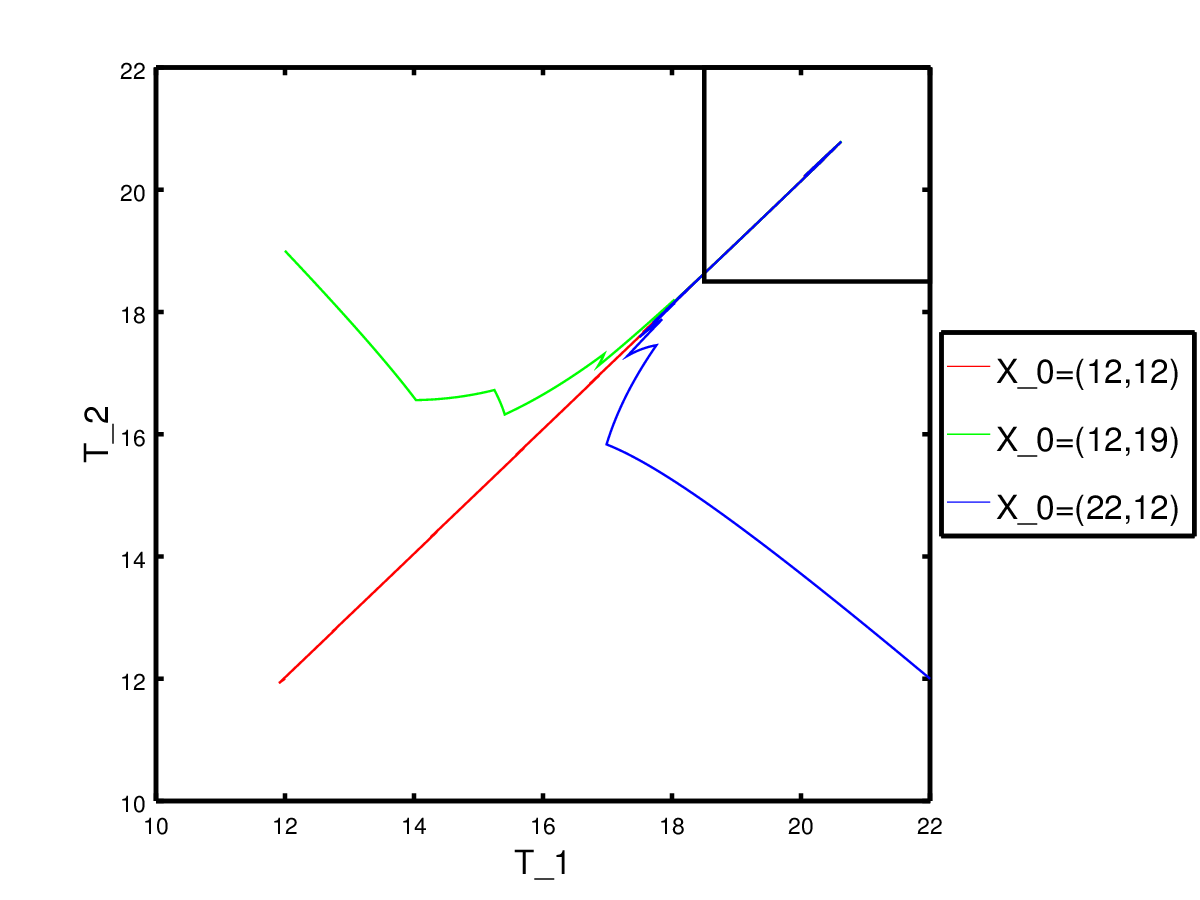
\includegraphics[trim = 0cm 0.3cm 0cm 1cm, clip, width=0.4\textwidth]{simu_distributed_2rooms_state.png}
%   &
\qquad
   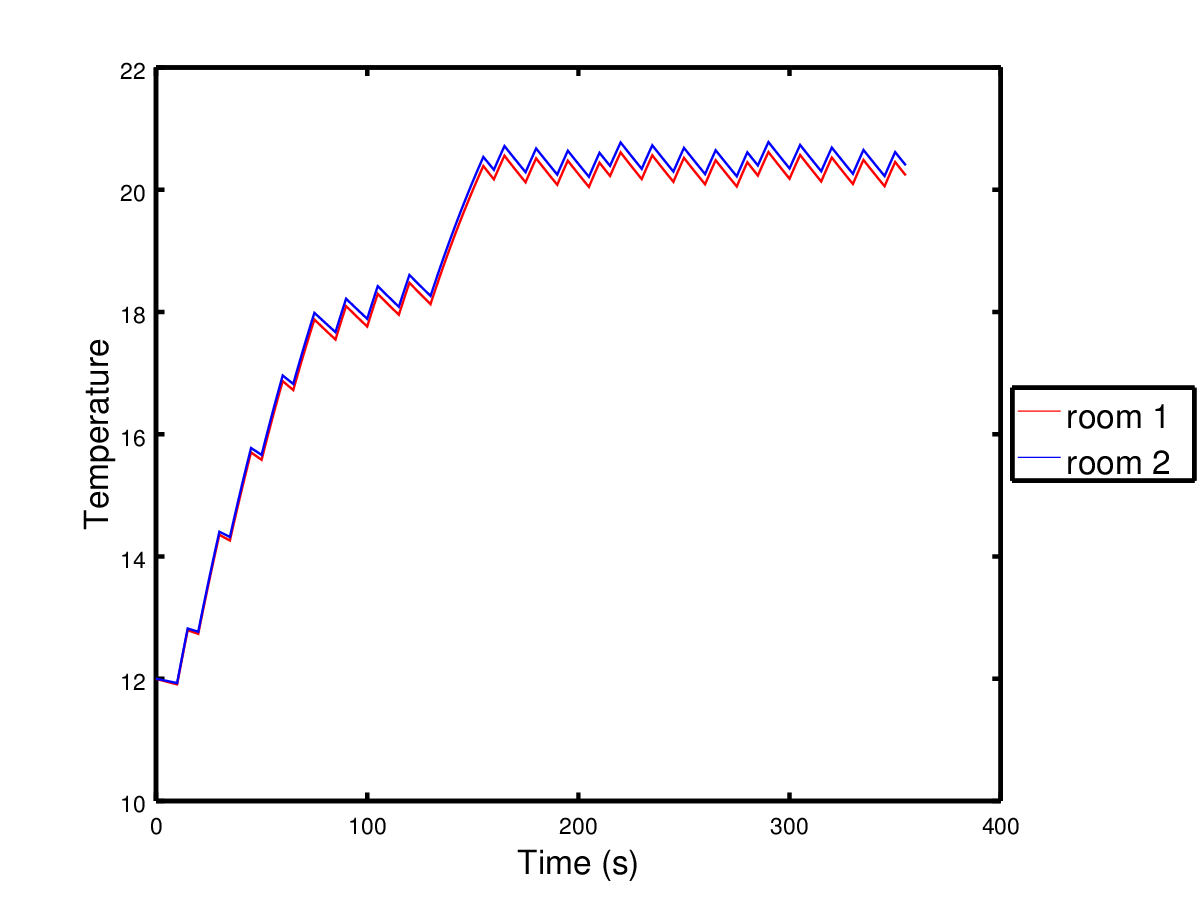
\includegraphics[trim = 0cm 0.3cm 0cm 1cm, clip, width=0.4\textwidth]{simu_distributed_2rooms_time.png}
%  \end{tabular}

  \caption{Simulations of the distributed reachability controller for three different initial conditions plotted
  in the state space plane (left); simulation of the distributed reachability controller for the initial condition $(12,12)$ plotted 
  within time (right).}
 \label{fig:simu_distri}
\end{figure}

% \begin{figure}[!h]
%   \centering
% 
%   \caption{.}
%  \label{fig:simu_distri_time}
% \end{figure}
% 
 \end{example}

%\section{Case where $f_1$ and $f_2$ are affine}

\subsection{Case Study}
\label{sec:case_study0}

This case study, proposed by the Danish company Seluxit, aims at controlling 
the temperature of an eleven rooms house, heated by geothermal energy.
%We manage to synthesize a correct-by-construction control for this 
%example.
The~\emph{continuous} dynamics of the system is the following:
\begin{equation}
 \frac{d}{dt} T_i(t) = \sum_{j=1}^n A_{i,j}^d (T_j(t) - T_i(t)) + B_i(T_{env} (t) - T_i(t)) + H_{i,j}^v.v_j 
\end{equation}



The temperatures of the rooms are the $T_i$.  The matrix $A^d$
contains the heat transfer coefficients between the rooms, matrix $B$
contains the heat transfer coefficients betweens the rooms and the
external temperature, set to ${T_{env} = 10^\circ C}$ for the
computations. The~control matrix~$H^v$ contains the effects of the
control on the room temperatures, and the control variable is here
denoted by~$v_j$. We~have $v_j = 1$ (resp.~$v_j = 0$) if the heater in
room~$j$ is turned on (resp.~turned~off). We~thus have $n=11$ and
$N=2^{11} = 2048$ switching modes.


Note that the matrix $A^d$ is parametrized by the open of closed state
of the doors in the house. In our case, the average between closed and
open matrices was taken for the computations. The exact values of the
coefficients are given in~\cite{larsen2015online}.  The controller has
to select which heater to turn on in the eleven rooms. Due to a
limitation of the capacity supplied by the geothermal device, the~$11$
heaters cannot be turned on at the same time.  In~our case, we~limit
to~$4$ the number of heaters that can be on at the same time.


%--------
We consider the distributed control synthesis problem where
the first (resp. second) state component corresponds to 
the temperatures of rooms~1 to~5 (resp.~6 to~11),
and the first (resp. second) control mode component corresponds to the heaters 
of rooms~1 to~5 (resp.~6 to~11).
Hence $n_1=5, n_2=6, N_1=2^5, N_2=2^6$. We~impose
that at most two heaters are switched on at the same time in the
first sub-system, and at most two in the second sub-system.

Let $D=1$ (the bisection depth is at most~1),
and $K=4$ (the maximum length of patterns is~4).
The parameter $\varepsilon$ is set to value $0.5^\circ C$.
The sampling time is $\tau=15$ minutes.


We look for a distributed controller 
which steers any temperature state in
the rectangle $S=[18-a,22]^{11}$
to $R=[18,22]^{11}$ with $a$ as large as possible, 
then maintain the temperatures in~$R$ indefinitely.
%
Using our implementation, the computation of the control synthesis
takes around 20 hours of CPU time.
%
The method iterates the macro-step control synthesis procedure 15
times.  We~find $S=[18-a,22]^{11}$ with $a=4.2$, i.e.
$S=[13.8,22]^{11}$.  This means that any element of~$S$ can be driven
into~$R$ within 15 macro-steps of length (at~most)~4, i.e., within
$15\times 4=60$ units of time.  Since each time unit is of duration
$\tau=15$ min, any trajectory starting from~$S$ reaches~$R$ within
$60\times 15=900$ min.  The~trajectory is then guaranteed to stay in
$R+(\varepsilon,\varepsilon)=[17.5,22.5]^{11}$.
%
These results are consistent with the simulation given in
Figure~\ref{fig:reach_11rooms_10} showing the time evolution of the
temperature of the rooms, starting from~$14^{11}$.

%Robustness simulations for our controller
%are given in Appendix \ref{sec:robustness}.



\begin{figure}[t]
  \centering
 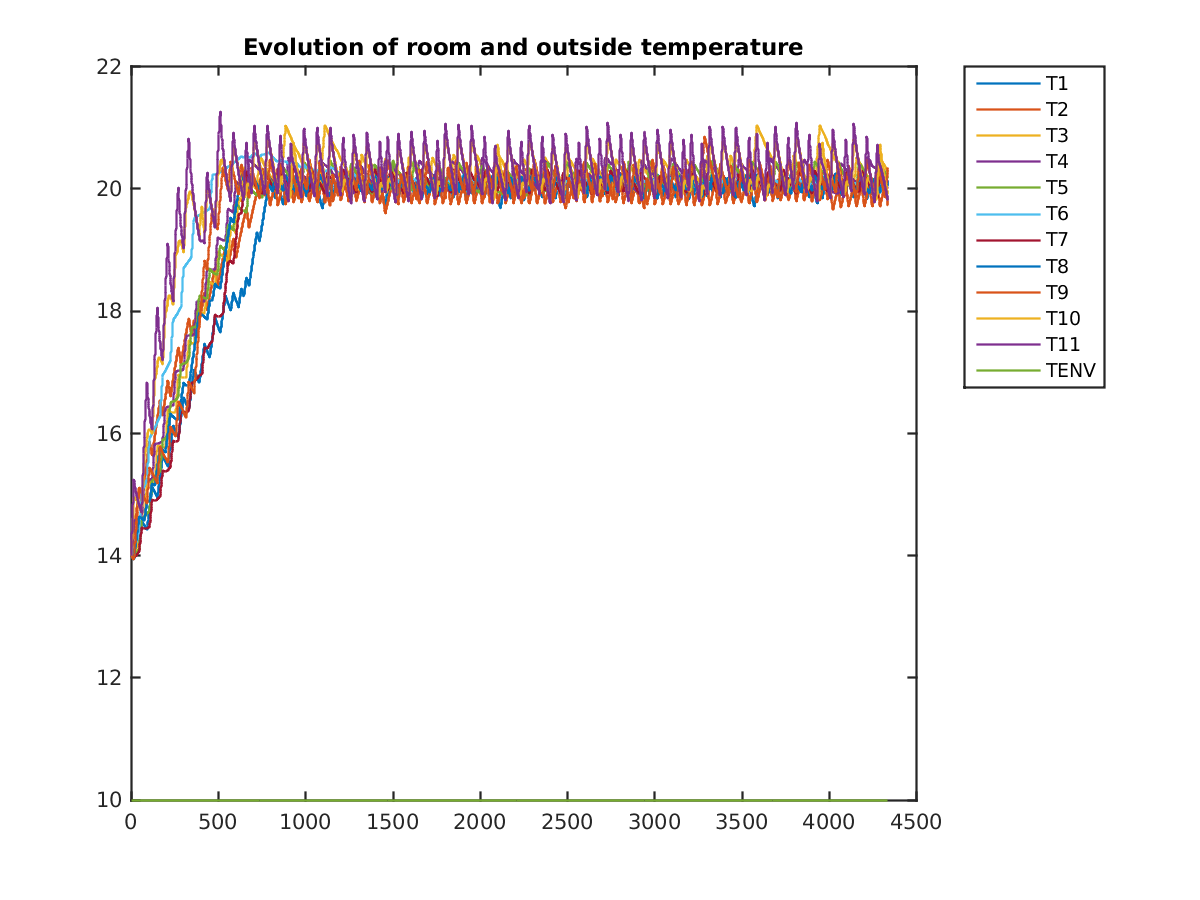
\includegraphics[trim = 0cm 1cm 0cm 0cm, clip, scale = 0.4]{reachability_11rooms_synchronized_10_degrees.png}
 \caption{Simulation of the Seluxit case study 
plotted with time (in min) for $T_{env}=10^{\circ} C$.}
 \label{fig:reach_11rooms_10}
\end{figure}



\subsubsection{Robustness Experiments}\label{sec:robustness}


We now perform the same simulations as in Figure \ref{fig:reach_11rooms_10}, except 
that the environment temperature is not fixed at $10^\circ$C but follows
scenarios of soft winter (Figure~\ref{fig:reach_11rooms}) and spring 
(Figure \ref{fig:reach_11rooms_stab}). The environment temperature is plotted
in green in the figures. The spring scenario is taken from \cite{larsen2015online},
and the soft winter scenario is the winter scenario 
of \cite{larsen2015online} with $5$ additional degrees.
We see that our controller, which is designed for $T_{env} = 10^\circ$C still
satisfies the properties of reachability and stability. These simulations 
are very close those obtained in~\cite{larsen2015online}.

\begin{figure}[ht]
  \centering
 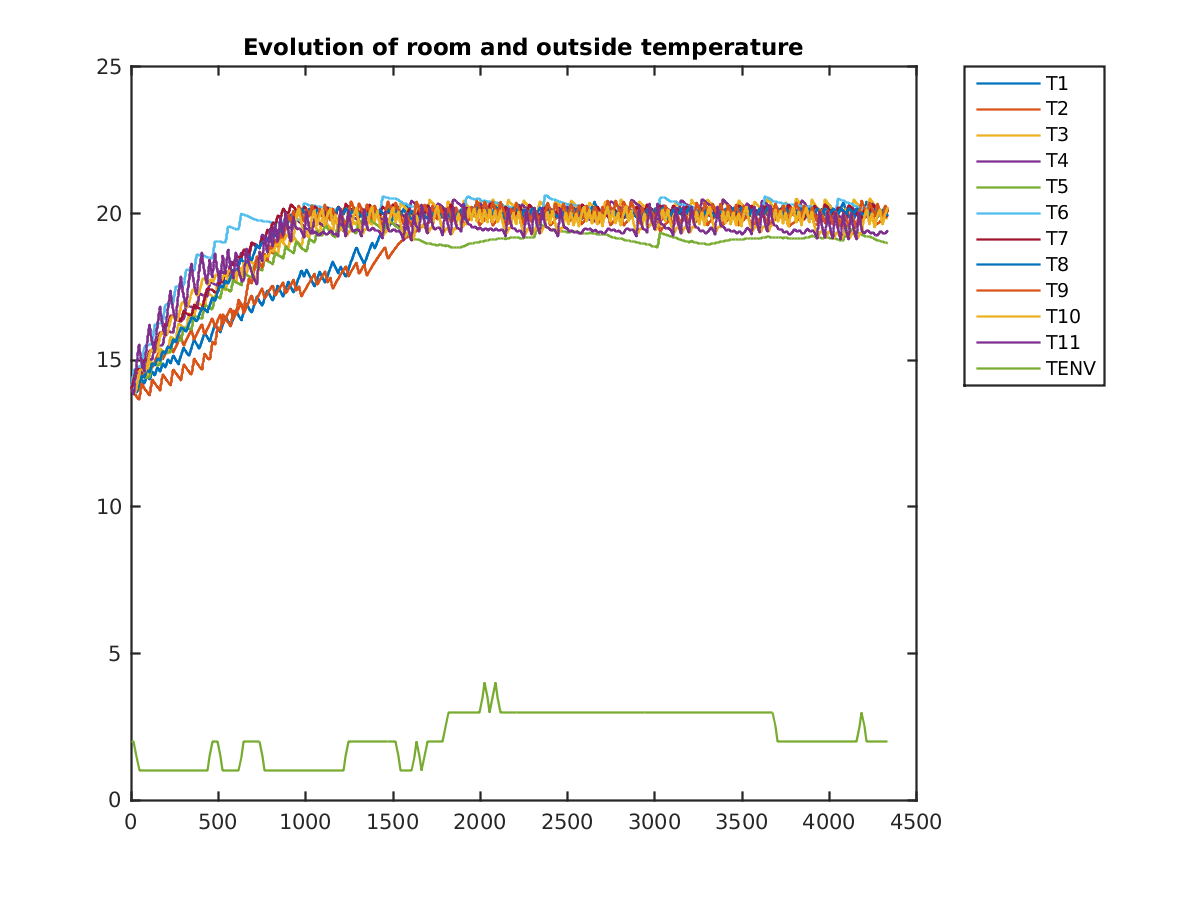
\includegraphics[trim = 0cm 1cm 0cm 0cm, clip, scale = 0.4]{reachability_11rooms.png}
 \caption{Simulation of the Seluxit case study in the soft winter scenario.}
 \label{fig:reach_11rooms}
\end{figure}


\begin{figure}[ht]
  \centering
 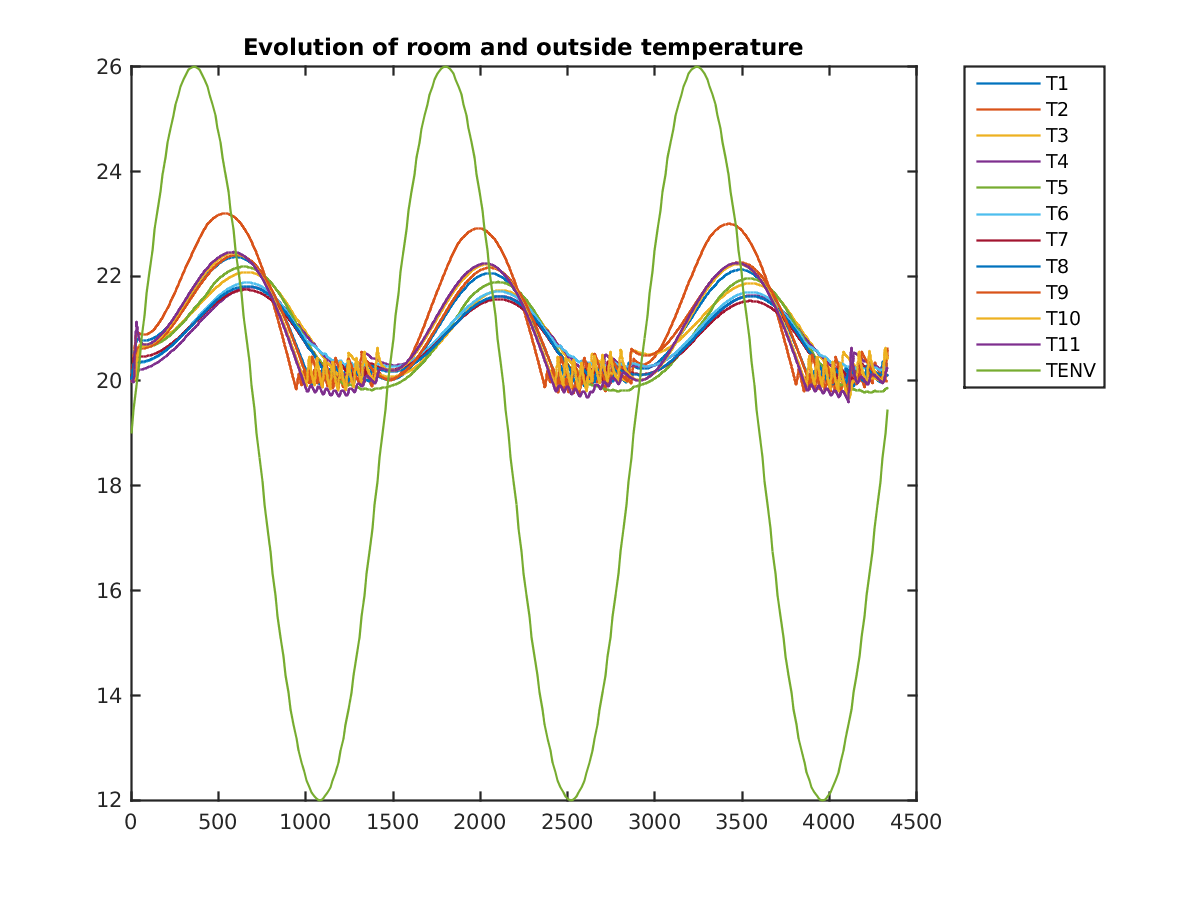
\includegraphics[trim = 0cm 1cm 0cm 0cm, clip, scale = 0.4]{stability_11rooms.png}
 \caption{Simulation of the Seluxit case study in the spring scenario.}
 \label{fig:reach_11rooms_stab}
\end{figure}

%%%%% fin copie de l'annexe









\subsection{Continuous-time case}
%\label{sec-nonilnear}
\label{sec-continuous}
In this section, we consider the case of continuous-time differential equations.
The~time~$t$ now takes its value in~$\mathbb{R}_{\geq 0}$.
\subsection{Reachability in continuous time}
Consider the continuous-time system with \emph{finite control}:
\begin{xalignat}1
 \dot{x}_1(t) &= f_1(x_1(t),x_2(t),u_1) \label{eq:nl_sys1} \\
 \dot{x}_2(t) &= f_2(x_1(t),x_2(t),u_2) 
 \label{eq:nl_sys2}
\end{xalignat}
where $x_1$ (resp.~$x_2$) is the first (resp. second)  component
of the state vector variable, taking its values
in $\mathbb{R}^{n_1}$ (resp.~$\mathbb{R}^{n_2}$), 
and where $u_1$ (resp.~$u_2$) is
the first (resp.~second) component of the control \emph{mode},
taking its values in the \emph{finite} set~$U_1$ (resp.~$U_2$).
We will often write~$x$ for $(x_1,x_2)$, $u$~for~$(u_1,u_2)$,
and $n$ for~$n_1+n_2$.
We will also abbreviate the set $U_1\times U_2$ as~$U$.
%
%Let $N$ be the cardinal of $U$, and $N_1$ (resp. $N_2$) the cardinal
%of $U_1$ (resp. $U_2$). We have $N=N_1 \cdot N_2$.
%
We~abbreviate the continuous-time system under
the form:
%
\begin{equation}
\dot{x}(t)=f(x(t),u)
\label{eq:nl_sys_central}
\end{equation}
%
where $x$ is a vector state variable taking its values in
$\mathbb{R}^n=\mathbb{R}^{n_1}\times \mathbb{R}^{n_2}$, and where
$u$~is of the form $(u_1,u_2)$, with $u_1$ taking its values in $U_1$
and $u_2$ in~$U_2$.  We~assume that, given an initial value~$x_0$,
Equation~\eqref{eq:nl_sys_central} has a solution
%
(e.g., assuming that the vector field~$f$ (resp.~$f_1$,~$f_2$) is
Lipschtiz).


We define the reachable set of~\eqref{eq:nl_sys_central} from a set of
initial states $X_0$, at time $t$ $(0\leq t\leq \tau)$ under control
mode~$u$:
%
\[
\Reach_f(t,X_0,u)=\{\Phi(t,x_0,u) \ |\ x_0\in X_0\}.
\]
%
where $\Phi(t, x,u)$ denotes the state $x(t)$ reached at time $t$
$(0\leq t\leq \tau)$ starting from the initial state~$x$, under
control mode $u\in U$.


%\fbox{factoriser les deux paragraphes suivants}
We define the reachable set of \eqref{eq:nl_sys1} from a set of initial states
$X_1\subset \mathbb{R}^{n_1}$, at time $t$ $(0\leq t\leq \tau)$ under control mode $u_1\in U_1$ and perturbation $X_2\subset \mathbb{R}^{n_2}$:
%
\[
\Reach_{f_1}(t,X_1,X_2,u_1)=\{\Phi_1(t,x_1,X_2,u_1) \ |\ x_1\in X_1\}.
\]
%
where
$\Phi_1(t, x_1,X_2,u_1)$ is the set of states $x_1(t)$ reached at time 
$t$ $(t\geq 0)$ from the initial 
state $x_1$, under control mode $u_1$ and perturbation $X_2$.

Symmetrically, we
define the reachable set of \eqref{eq:nl_sys2} from a set of initial states
$X_2\subset \mathbb{R}^{n_2}$, at time $t$ $(0\leq t\leq \tau)$ under control mode $u_2\in U_2$ and perturbation $X_1\subset \mathbb{R}^{n_1}$:
%
\[
\Reach_{f_2}(t,X_1,X_2,u_2)=\{\Phi_2(t,X_1,x_2,u_2) \ |\ x_2\in X_2\}.
\]
%
where
$\Phi_2(t, X_1,x_2,u_2)$ is the set of states $x_2(t)$ reached at time 
$t\geq 0$ from the initial 
state $x_2$, under control mode $u_2$ and perturbation $X_1$.

All the notions of reachable sets for modes are extended in the
natural manner to the notions of reachable sets for \emph{patterns}. 
For example, for the pattern $\pi=u\cdot v$ of
length~$2$, and for $0\leq t\leq \tau$, we~define:
\begin{xalignat*}1
  \Reach_f(t,X_0,\pi) & = \Reach_f(t,X_0,u)
  %\text{ for $0\leq t\leq \tau$
  \\
  \Reach_f(\tau+t,X_0,\pi) & = \Reach_f(t,X_1,v)
  %for $0\leq t\leq \tau$,
 \qquad\text{with $X_1=\Reach_f(\tau,X_0,u)$.}
\end{xalignat*}



%We suppose that we are able to compute an overapproximation
%of the reachable set denoted $\overline{\Reach}$. 




\subsubsection{Distributed control}
Recall that $\pi_1^k$ (resp. $\pi_2^k$) denotes the prefix of length $k$
of $\pi_1$ (resp.$\pi_2$), and $\pi_1(k)$ (resp. $\pi_2(k)$)
the $k$-th element of sequence $\pi_1$ (resp. $\pi_2$).
We now give the counterpart of Definition \ref{def:1}.
\begin{definition}
Consider an element $r_{i_1}$ (resp. $r_{i_2}$) of a tiling ${\cal R}_1$
(resp. ${\cal R}_2$) of $R_1$
(resp. $R_2$), and a sequence $\pi_1\in\Pi_1^{\leq K}$ (resp. $\pi_2\in\Pi_2^{\leq K}$)
of length $\ell_1$ (resp. $\ell_2$).
The \emph{approximate first-component sequence}
$\{Y^k_{i_1}(a,\pi_1)\}_{0\leq k\leq \ell_1}$ 
is defined as follows:
\begin{itemize}
\item $Y^0_{i_1}(a,\pi_1)=r_{i_1}+a$ and 
\item $Y^{k}_{i_1}(a,\pi_1)=\bigcup_{0\leq t\leq \tau}\Reach_{f_1}(t,Y^{k-1}_{i_1}(a,\pi_1),R_2+a+\varepsilon,\pi_1(k))$ for ${1\leq k\leq \ell_1}$.
%
\end{itemize}
Similarly, the \emph{approximate second-component sequence} $\{Y^k_{i_2}(a,\pi_2)\}_{0\leq k\leq \ell_2}$ is defined by
\begin{itemize}
\item $Y^0_{i_2}(a,\pi_2)=r_{i_2}+a$ and 
\item $Y^{k}_{i_2}(a,\pi_2)=\bigcup_{0\leq t\leq \tau}\Reach_{f_2}(t,R_1+a+\varepsilon,Y^{k-1}_{i_2}(a,\pi_2),\pi_2(k))$
for ${1\leq k\leq\ell_2}$.
\end{itemize}
%
\end{definition}
%

We define the property
%
$\Prop_1(a,i_1,\pi_{1})$ by:
%$\{Y^{k}_1\}_{0\leq k\leq \ell_1}$ such that:
%\begin{itemize}
%\item
\begin{center}
  $Y^{k}_{i_1}(a,\pi_{1})\subseteq R_1+a+\varepsilon$ for $1\leq k\leq \ell_{1}$\par
  and
  %\item
  $\Reach_{f_1}(\ell_1\tau,r_{i_1}+a,R_2+a+\varepsilon,\pi_{1})\subseteq R_1$.
\end{center}
%\end{itemize}
%
Likewise, we define the property
%
$\Prop_2(a,i_2,\pi_{2})$ by:
%$\{Y^{k}_1\}_{0\leq k\leq \ell_1}$ such that:
%\begin{itemize}
%\item
\begin{center}
  $Y^{k}_{i_2}(a,\pi_{2})\subseteq R_2+a+\varepsilon$ for $1\leq k\leq \ell_{2}$\par
  and
  %\item
  $\Reach_{f_2}(\ell_2\tau,R_1+a+\varepsilon,r_{i_2}+a,\pi_{2})\subseteq R_2$.
\end{center}
%\end{itemize}

Assumptions $H1(\ell_1)$, $H_2(\ell_2)$ and expressions 
$A$, 
$\pi_{i_1}$, $\pi_{i_2}$
are defined exactly
as in Section~\ref{ss:macro_dist}.
%
We now give the counterpart of Lemma \ref{prop:lemma} 
(the proof is similar).

\begin{lemma}\label{prop:lemma2}
Consider a tiling ${\cal R}={\cal R}_1\times{\cal R}_2$ of the
form $\{r_{i_1}\times r_{i_2}\}_{(i_1,i_2)\in I_1\times I_2}$.
% Let $i_1\in I_1, i_2\in I_2$ and $a>0$.
Suppose that $H1(\ell_1)$ and
$H2(\ell_2)$ hold, for some positive real $\varepsilon$, 
and some positive integers $\ell_1, \ell_2$.
%(i.e: for all $i_1 \in I_1$, $\Prop(a,i_1,\pi_{1})$
%holds for some $\pi_{1}\in \Pi_1^{\ell_1}$, and for all $i_2 \in
%I_2$, $\Prop(a,i_2,\pi_{2})$ holds for some
%$\pi_{2}\in \Pi_2^{\ell_2}$).
Then we have

\begin{itemize}
\item in case $\ell_1\leq \ell_2$, for all $t\in [(k-1)\tau, k\tau]$
($1\leq k\leq \ell_1$):
%\fbox{for all $k\leq \ell_1$ and $t$ such that ... ???}
  \begin{xalignat*}1
  \Reach_f(t,(r_{i_1}+A) \times (R_2+A),(\pi_{i_1}^k,\pi_{i_2}^k))_{|1}\subseteq Y_{i_1}^k(a,\pi_{i_1})
& \subseteq R_1+A+\varepsilon
\\
\Reach_f(t,(R_1+A)\times(r_{i_2}+A),(\pi_{i_1}^k,\pi_{i_2}^k))_{|2}\subseteq Y_{i_2}^k(a,\pi_{i_2})
&\subseteq R_2+A+\varepsilon 
\\
%\hspace*{\fill}for all $1\leq k\leq \ell_1$, and
%
\Reach_f(\ell_1\tau,(r_{i_1}+A)\times( R_2+A),(\pi_{i_1}^{\ell_1},\pi_{i_2}^{\ell_1}))_{|1}%\subseteq Y_{i_1}^{\ell_1}(a,\pi_{i_1})
& \subseteq R_1.
\end{xalignat*}

\item in case $\ell_2 \leq \ell_1$, for all $t \in [(k-1)\tau, k\tau]$
$(1\leq k\leq \ell_2)$:
%\fbox{for all $k\leq \ell_1$ and $t$ such that ... ???}
\begin{xalignat*}1
\Reach_f(t,(r_{i_1}+A)\times( R_2+A),(\pi_{i_1}^k,\pi_{i_2}^k))_{|1}\subseteq Y_{i_1}^{k}(a,\pi_{i_1})
&\subseteq R_1+A+\varepsilon
\\
\Reach_f(t,(R_1+A)\times(r_{i_2}+A),(\pi_{i_1}^k,\pi_{i_2}^k)){|_2}\subseteq Y_{i_2}^k(a,\pi_{i_2})
&\subseteq R_2+A+\varepsilon
\\
%\hspace*{\fill}for all $1\leq k\leq \ell_2$, and
\Reach_f(\ell_2\tau,(R_1+A)\times(r_{i_2}+A),(\pi_{i_1}^{\ell_2},\pi_{i_2}^{\ell_2}))_{|2}%\subseteq Y_{i_2}^{\ell_2}(a,\pi_2)
& \subseteq R_2.
\end{xalignat*}





\end{itemize}

\end{lemma}

We now give the counterpart of Theorem \ref{th:1_part3} (the proof is similar).

\begin{theorem}\label{th:2}
%Suppose that there is a tiling ${\cal R}={\cal R}_1\times{\cal R}_2$ 
%of $R$ of the
%form $\{r_{i_1}\times r_{i_2}\}_{(i_1,i_2)\in I_1\times I_2}$.
Suppose that there is a tiling ${\cal R}_1=\{r_{i_1}\}_{i_1\in I_1}$ of $R_1$
and a tiling ${\cal R}_2=\{r_{i_2}\}_{i_2\in I_2}$ of $R_2$,
%Suppose that there is a tiling 
%${\cal R}={\cal R}_1\times{\cal R}_2$ of $R$, 
%and a positive real $\varepsilon$
such that
$H1(\ell_1)$ and $H2(\ell_2)$ hold
for some $\ell_1,\ell_2 \leq K$.
Let $\ell=lcm(\ell_1,\ell_2)$ with $\ell=\alpha_1 \ell_1=\alpha_2 \ell_2$
for some $\alpha_1,\alpha_2\in \mathbb{N}$.
%Consider the situation described in Proposition \ref{prop:basic}.
%Suppose furthermore that
%$| \pi_{1} | = |\pi_{j_1}|=\ell_1$ for all $i_1,j_1\in I_1$, and
%%
%$| \pi_{2} | = |\pi_{j_2}|=\ell_2$ for all $i_2,j_2\in I_2$.

Then
%, starting from a point $x=(x_1,x_2)\in (R_1+a)\times (R_2+a)$, 
${\cal R}_1$ induces a 
sequence of $\alpha_1$ macro-steps on $R_1+A$, and ${\cal R}_2$
a sequence of $\alpha_2$ macro-steps on $R_2+A$, such that, 
when applied concurrently, we have
for all $i_1\in I_1$ and $i_2\in I_2$:
%macro-step\footnote{pas exactement ``one'',
%mais $lcm(\ell_1,\ell_2)$ divis\'e par $\ell_1$ and $\ell_2$ respectivement} reachability uniform
%distributed control
%of horizon $K$ 
\begin{multline*}
\Reach_f(\ell \tau,(r_{i_1}+A)\times (R_2+A),\pi)_{|1}\subseteq R_1 \ \wedge\\ 
\Reach_f(\ell \tau,(R_1+A)\times (r_{i_2}+A),\pi)_{|2}\subseteq R_2,
\end{multline*}
%$$ f(x,\pi)\in R,$$
%, \mbox{ i.e., } f((x_1,x_2),(\pi_1^1\cdot \cdots \cdot\pi_1^{\alpha_1},
%\pi_2^1\cdot \cdots \cdot\pi_2^{\alpha_2}))\in R_1\times R_2.$$
for some $\pi=(\pi_1,\pi_2)\in \Pi^{\ell}$ where $\pi_1$ (resp. $\pi_2$)
is of the form $\pi_1^1\cdots \pi_1^{\alpha_1}$
(resp. $\pi_2^1\cdots \pi_2^{\alpha_2}$)
with $\pi_1^i\in \Pi_1^{\ell_1}$  for all $1\leq i\leq \alpha_1$
(resp. $\pi_2^i\in \Pi_2^{\ell_2}$  for all $1\leq i\leq \alpha_2$).
%
Hence:
$$\Reach_f(\ell\tau,r_{i_1,i_2}+(A,A),\pi)\subseteq R.$$
Besides, for all $0\leq t \leq \ell\tau$,
we have:
\begin{multline*}
  \Reach_f(t,(r_{i_1}+A)\times (R_2+A),\pi)_{|1}\subseteq R_1+A+\varepsilon\\ 
  \wedge\ \Reach_f(t,(R_1+A)\times (r_{i_2}+A),\pi)_{|2}\subseteq R_2+A+\varepsilon.
\end{multline*}
%
%$$f(x,\pi')\in R+(a+\varepsilon,a+\varepsilon).$$
Hence, for all $0\leq t \leq \ell\tau$:
$$\Reach_f(t,r_{i_1,i_2}+(A,A),\pi)\subseteq R+(A+\varepsilon,A+\varepsilon).$$
\end{theorem}


Theorem \ref{th:2} allows us to implement the method along the same lines as in the discrete-time case, except that we apply the operator $Reach_{f_1}$ and $Reach_{f_2}$
on continuous time intervals of the form $[k,(k+1)\tau]$
instead of the mappings $f_1$ and $f_2$ at times $k\tau$.
We have implemented the method
using the system $DynIBEX$
\cite{dynibex,dit2016validated} which makes use of interval arithmetic \cite{Moore66}
and Runge-Kutta methods to compute
(an overapproximation of)
the application results of 
$Reach_{f_1}$ and $Reach_{f_2}$.

\subsubsection{Application}


We demonstrate the feasibility of our approach on a building
ventilation application adapted from~\cite{meyer:tel-01232640}.
The~system is a four-room apartment subject to heat transfer between
the rooms, with the external environment, with the underfloor, and
with human beings.  The dynamics of the system is given by the
following equation:
\begin{multline}
 \frac{d T_i}{dt} = \sum_{j \in \mathcal{N}^\text{*}\setminus \{i\}} a_{ij} (T_j -
 T_i) + \delta_{s_i} b_i (T_{s_i}^4 - T_i ^4 ) \\ + c_i
 \max\left(0,\frac{V_i - V_i^\text{*}}{\bar{ V_i} -
   V_i^{\text{*}}}\right)(T_u - T_i).
\end{multline}

The state of the system is given by the temperatures in the rooms
$T_i$, for $i \in \mathcal{N} = \{ 1 , \dots , 4 \}$.  Room $i$ is
subject to heat exchange with different entities stated by the indexes
$\mathcal{N}^\text{*} = \{1,2,3,4,u,o,c \}$.
%
The heat
transfer between the rooms is given by the coefficients $a_{ij}$ for
$i,j \in  \mathcal{N}^2$, and the different perturbations are the following:
\begin{itemize}
 \item The external environment: it has an effect on room $i$ with the
   coefficient $a_{io}$ and the outside temperature $T_o$, varying
   between $27^\circ C$ and $30^\circ C$.
  \item The heat transfer through the ceiling: it has an effect on
    room $i$ with the coefficient $a_{ic}$ and the ceiling temperature
    $T_c$, varying between $27^\circ C$ and $30^\circ C$.
  \item The heat transfer with the underfloor: it is given by the
    coefficient $a_{iu}$ and the underfloor temperature $T_u$, set to
    $17^\circ C$ ($T_u$ is constant, regulated by a PID controller).
  \item The perturbation induced by the presence of humans: it is
    given in room $i$ by the term $\delta_{s_i} b_i (T_{s_i}^4 - T_i
    ^4 )$, the parameter $\delta_{s_i}$ is equal to $1$ when someone
    is present in room $i$, $0$ otherwise, and $T_{s_i}$ is a given
    identified parameter.
\end{itemize}

The control $V_i$, $i \in \mathcal{N}$, is applied through the term
$c_i \max(0,\frac{V_i - V_i^\text{*}}{\bar{ V_i} -
  V_i^{\text{*}}})(T_u - T_i)$.  A voltage $V_i$ is applied to force
ventilation from the underfloor to room $i$, and the command of an
underfloor fan is subject to a dry friction.  Because we work in a
switching control framework, $V_i$ can take only discrete values, which
removes the problem of dealing with a ``max'' function in interval
analysis. In the experiment, $V_1$ and $V_4$ can take the values $0$V
or $3.5$V, and $V_2$ and $V_3$ can take the values $0$V or $3$V. This
leads to a system of the form~\eqref{eq:nl_sys_central} with $u(t) \in U =\{
1, \dots, 16 \}$, the $16$ switching modes corresponding to the
different possible combinations of voltages $V_i$. The system can be decomposed in
sub-systems of the form \eqref{eq:nl_sys1}-\eqref{eq:nl_sys2}. The sampling
period is $\tau = 10$s.


The parameters $T_{s_i}$, $V_i^\text{*}$, $\bar V_i$, $a_{ij}$, $b_i$,
$c_i$ are given in~\cite{meyer:tel-01232640} and have been identified
with a proper identification procedure detailed
in~\cite{meyer2014ecc}.  Note that here we have neglected the term
$\sum_{j \in \mathcal{N}} \delta_{d_{ij}}c_{i,j} \ast h(T_j - T_i)$
of~\cite{meyer:tel-01232640}, representing the perturbation induced by
the open or closed state of the doors between the rooms. Taking a
``max'' function into account with interval analysis is actually still
a difficult task. However, this term could have been taken into
account with a proper regularization (smoothing).

The main difficulty of this example is the large number of modes in
the switching system, which induces a combinatorial issue.
%
%\fbox{parler de l'impl\'ementation, de la biblioth\`eque utilis\'ee...}
The centralized controller was obtained with $704$ tiles in $29$
minutes, the distributed controller was obtained with $16 + 16$ tiles
in $20$ seconds. In both cases, patterns of length $1$ are used. The
perturbation due to human beings has been taken into account by
setting the parameters $\delta_{s_i}$ equal to the whole interval
$\lbrack 0,1 \rbrack$ for the decomposition, and the imposed
perturbation for the simulation is given
Figure~\ref{fig:NL_2_part3_perturbation_part3}.  The temperatures $T_o$ and $T_c$
have been set to the interval $\lbrack27,30\rbrack$ for the
decomposition, and are set to $30^\circ C$ for the simulation.  A
simulation of the controller obtained with the state-space bisection
procedure is given in Figure~\ref{fig:NL_2_part3}, where the control
objective is to stabilize the temperature in $\lbrack 20 , 22 \rbrack
^2 \times \lbrack 22 , 24 \rbrack^2$ while never going out of $\lbrack
19 , 23 \rbrack ^4 \times \lbrack 21 , 25 \rbrack ^4$.


\begin{figure}[ht]
 \centering
 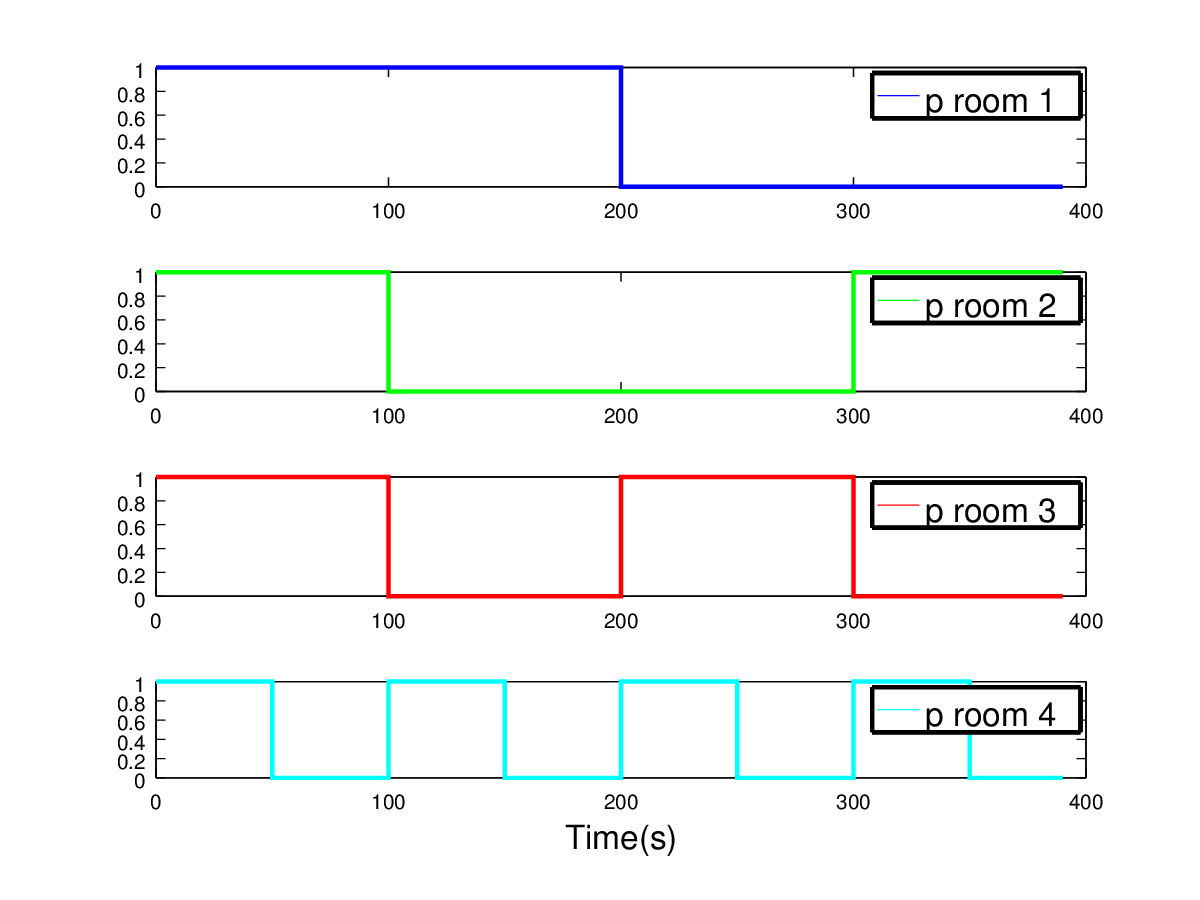
\includegraphics[scale=0.4]{NL_case_2_perturbation.png}
 \caption{Perturbation (presence of humans) imposed within time in the
   different rooms.}
  \label{fig:NL_2_part3_perturbation_part3}
\end{figure}


\begin{figure}[ht]
 \centering
 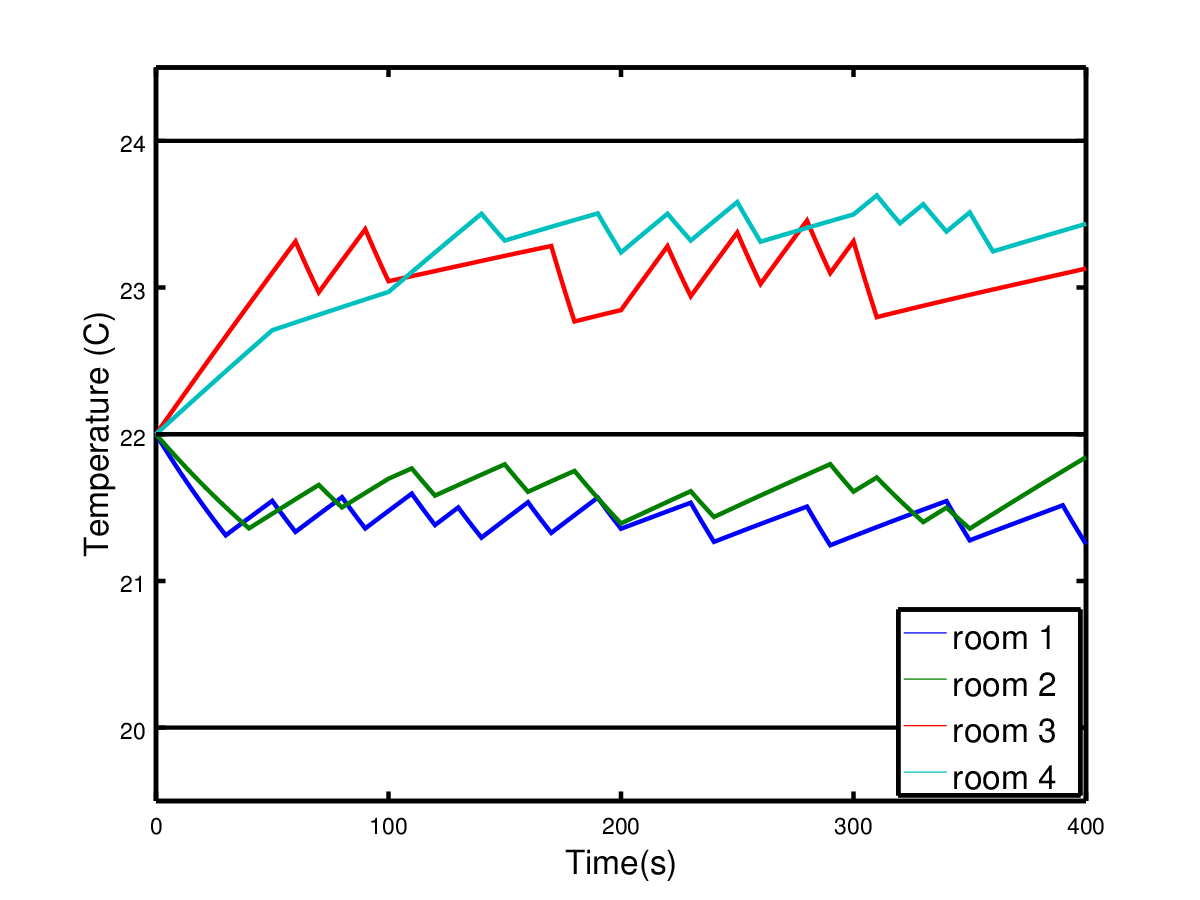
\includegraphics[scale=0.3]{compo_2objs2.png}%
% \caption{Simulation of the centralized controller from the initial condition $(22,22,22,22)$.}
%  \label{fig:NL_2_part3}
%\end{figure}
%
%\begin{figure}[ht]
% \centering
%\hfill
 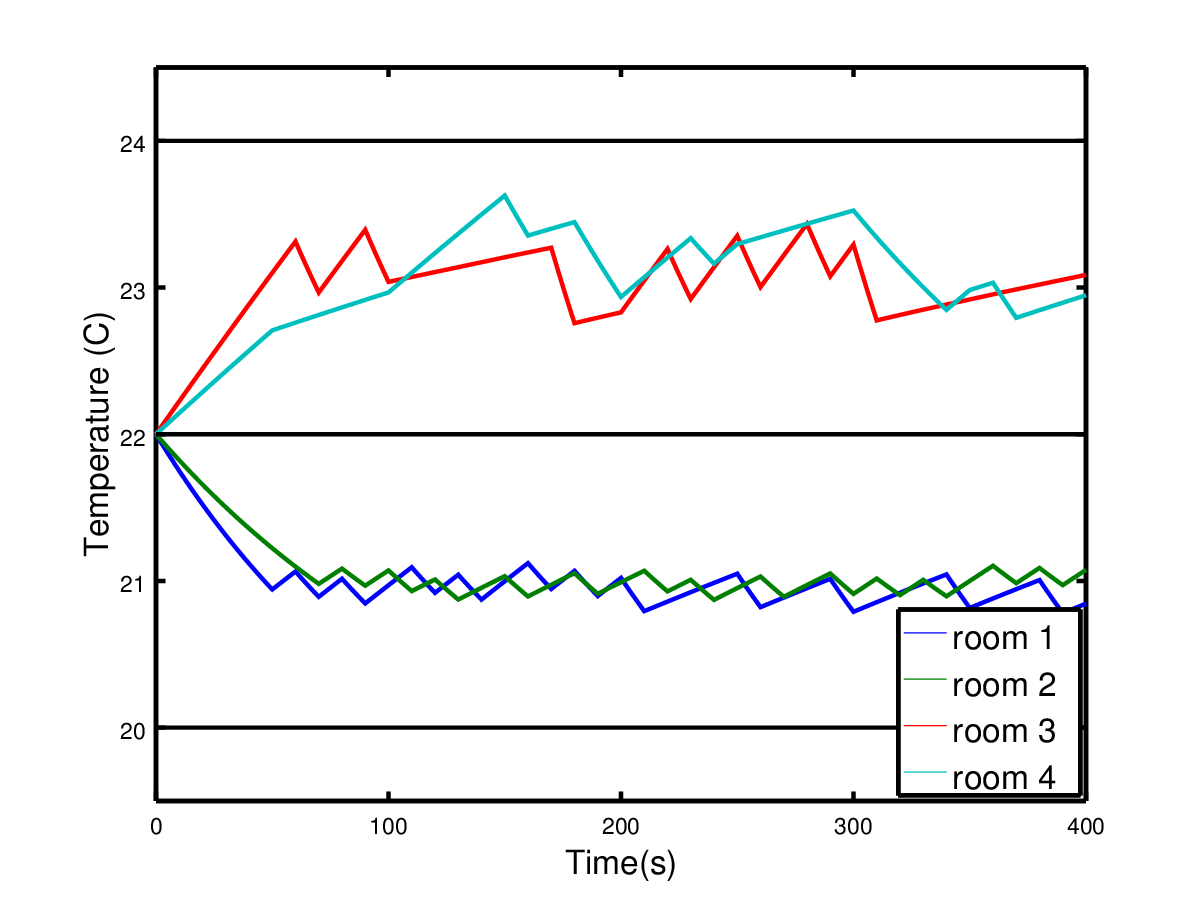
\includegraphics[scale=0.3]{compo_2objs3.png}
 \caption{Simulation of the centralized (left) and distributed (right) controllers from the initial condition $(22,22,22,22)$.}
  \label{fig:NL_2_part3}
\end{figure}

\subsection{Final Remarks}\label{sec:conc}

In this paper, we have proposed a distributed approach 
for control synthesis of sampled switching systems in the discrete-time framework
and applied it to a real floor heating system.
To our knowledge,
this is the first time that reachability and stability properties  
are guaranteed for a case study of this size. 
We have also explained how the method extends to the continuous-time framework.
The method can
be extended to take into account obstacles and safety constraints.

Note that it is essential in our method that the components are {\em sampled} with the {\em same} sampling period $\tau$, and that their clocks are synchronized.
It would be interesting to investigate how the approach behaves when clocks are badly synchronized or when they have different periods (see, e.g., \cite{KhatibGD16}).
%\fbox{Supprimer la phrase suivante, au moins...}
%We are currently investigating an 
%extension of the method to systems with non linear
%dynamics and varying parameters, see \cite{le2016control}. 




%\begin{remark}
%en fait vrai pour tout $0\leq t\leq k\tau$ (et pas seulement $0\leq t<k\tau$).
%\end{remark}
\section{Perturbed and distributed Euler scheme}

We consider the perturbed control system
\begin{equation}
  \dot x = f_j(x,d),
\end{equation}
where $d$ is assumed to belong to a given set $D$. 


In the same manner as the previous chapter, we introduce some additional
hypotheses allowing us to use an Euler's scheme with precise error bounds.
We suppose that the system is Lipschitz in the following sense:

For all $j \in U$, there exists a constant $L_j >0$ such that:
$$ \| f_{j} (x,d) - f_{j} (y,e) \| \leq L_j \left\| \begin{pmatrix} x \\ d \end{pmatrix} - \begin{pmatrix} y \\ e \end{pmatrix} \right\|, \quad \forall x,y \in S, \forall d,e \in D$$

We then introduce the constant:
$$ C_j = \sup_{x \in S} L_j \| f_j(x,d^m) \|$$
where $d^m$ denotes the center of box $D$. 

We now introduce a hypothesis similar to (H1) made in Chapter \ref{chap:2} (2), with additional
disturbance.

(H2) For every mode $j \in U$, there exists constants
$\lambda_j \in \mathbb{R}$ and $\gamma_j \in
\mathbb{R}_{>0}$ such that $\forall x,x' \in T$ and $\forall y,y'
\in D $, the following expression holds
$$ \langle f_j (x,y) - f_j (x',y'), x - x' \rangle \leq \lambda_j \| x - x' \|^2 + \gamma_j \| x - x' \| \| y - y' \|. $$

While the OSL condition is related to incremental stability, hypothesis (H2)
seems related to the notion of incremental input-to-state stability
(sometimes denotes $\delta$-ISS in the literature). Indeed, 
an incrementally input-to-state stable verifies a relation close to (H2), with 
a positive constant $\lambda_j$ (or more generally a $\kappa$). 
Here, we thus generalize this notion with negative constants $\lambda_j$.

\paragraph{Computation of constants $\lambda_j$ and $\gamma_j$, $L_j$ and $C_j$}

The computation of constants $L_j$, $C_j$, $\lambda_j$ 
($j\in U$) are realized with
a constrained optimization algorithm.
They are performed using the ``sqp'' function of Octave, applied on the following 
optimization problems:
\begin{itemize}
 \item Constant $L_j$ is computed exactly as in the unperturbed case:
 $$ L_j = \max_{{(x,d),(y,e)}\in S\times D,\  (x,d)\neq (y,e)} \frac{\| f_j(x,d) - f_j(y,e) \|}{\|\begin{pmatrix} x \\ d \end{pmatrix} - \begin{pmatrix} y \\ e \end{pmatrix} \|}  $$
 \item Constant $C_j$ is computed with the following optimization problem:
 $$ C_j = \max_{{x}\in S} L_j \| f_j(x,d^m) \|$$
 
 Knowing that: 
 $$ \langle f_j (x,y) - f_j (x',y'), x - x' \rangle =  \langle f_j (x,y) - f_j (x',y), x - x' \rangle + \langle f_j (x',y) - f_j (x',y'), x - x' \rangle$$
 
 \item Constant $\lambda_j$ is first computed as follows:
 $$ \lambda_j = \max_{{x,x'}\in T,\ y \in D,\  x\neq x'} \frac{\langle f_j(x,y) - f_j(x',y), x - x' \rangle}{\|x - x' \|^2 }$$
 \item Constant $\gamma_j$ is then computed:
  $$ \gamma_j = \max_{{x,x'}\in T, y,y' \in D,\  x\neq x' , y \neq y'} \frac{\langle f_j(x,y) - f_j(x',y'), x - x' \rangle - \lambda_j \| x - x' \|^2}{\|x - x' \|\|y-y'\| }$$
 \end{itemize}

 


\paragraph{Perturbed Euler's scheme}
 
We now define a perturbed Euler's scheme as follows:

\begin{eqnarray}
 \tilde x(\tau) = \tilde x(0) + \tau f_{j}(\tilde x(0),d^m)
\end{eqnarray}

% The exact trajectory is now denoted, for all $t \in [0,\tau]$, by
% $\phi_{(j_1,j_2)}(t;x^0)$ for an initial condition $x^0
% = \begin{pmatrix}x_1^0 & x_2^0\end{pmatrix}^T$, and when
% sub-system~$1$ is in mode $j_1 \in U_1$, and sub-system~$2$ is in mode
% $j_2 \in U_2$.

We define the approximate trajectory computed with the distributed
Euler scheme by $\tilde{\phi}_{j}(t;\tilde{x}^0) = \tilde x^0
+ t f_{j}(\tilde x^0,d^m)$ for $t \in [0,\tau]$, when the
system is in mode $j$ and with an initial condition $\tilde
x^0$. 

We now give a perturbed version of Theorem~\ref{th:1}.
\begin{theorem}\label{th:1_dist}
  Given a distributed sampled switched system, suppose that
  the system satisfies (H2), and consider a point $\tilde{x}^0$
  and a positive real $\delta$.
  % Let us denote by $\lambda_{j_1}$ the greatest eigenvalue of
  % $\frac{A_{j_1} + A_{j_1}^\top}{2}$ for all $j_1 \in U_1$.  Suppose
  % sub-system 1 verifies $$f_{\sigma_1}^1 (x_1,x_2) = A x_1 + B x_2 +
  % u_{\sigma_1}$$
  We have, for all $x^0\in B(\tilde{x}^0,\delta)$, $w : \R^+ \lra 
  D$, $t\in [0,\tau]$, $j\in U$:

  % $$\phi_j(t;x^0)\in B(\tilde{x}^0-t f_j(\tilde{x}^0), \gamma)$$
  $$\phi_{j}(t;x^0,w) \in B(\tilde{\phi}_{j}(t;\tilde{x}^0),\delta_{j}(t)).$$
  with, denoting by $| D |$ the diameter of $D$:
  \begin{itemize}
  \item if $\lambda_{j} <0$,
    \begin{multline}
      \delta_{j} (t) =
      % \frac{1}{\lambda_{j_1}^{3/2}}
      \left( \frac{(C_{j})^2}{-(\lambda_{j})^4} \left( - (\lambda_{j})^2 t^2 - 2 \lambda_{j} t + 2 e^{\lambda_{j} t} - 2 \right) \right.   \\
      + \left. \frac{1}{(\lambda_{j})^2} \left( \frac{C_{j} \gamma_{j} |D|}{-\lambda_{j}} \left( - \lambda_{j} t + e^{\lambda_{j} t} -1 \right) \right. \right.  \\ + \left. \left. \lambda_{j} \left( \frac{(\gamma_{j} )^2 (|D |/2)^2}{-\lambda_{j}} ( e^{\lambda_{j} t } - 1) + \lambda_{j} \delta^2 e^{\lambda_{j} t}  \right) \right)  \right)^{1/2}
    \end{multline}
\item if $\lambda_{j} >0$,
  \begin{multline}
    \delta_{j} (t) = \frac{1}{(3\lambda_{j})^{3/2}} \left( \frac{C^2}{\lambda_{j}} \left( - 9(\lambda_{j})^2 t^2 - 6\lambda_{j} t + 2 e^{3\lambda_{j} t} - 2 \right) \right.   \\
    + \left. 3\lambda_{j} \left( \frac{C \gamma_{j} |D|}{\lambda_{j}} \left( - 3\lambda_{j} t + e^{3\lambda_{j} t} -1 \right) \right. \right.  \\
    + \left. \left. 3\lambda_{j} \left( \frac{(\gamma_{j}) ^2 (|D|/2)^2}{\lambda_{j}} ( e^{3\lambda_{j} t } - 1) + 3\lambda_{j} \delta^2 e^{3\lambda_{j} t}  \right) \right)  \right)^{1/2}
  \end{multline}
\item if $\lambda_{j} = 0$,
  \begin{multline}
    \delta_{j} (t) =
    % \frac{1}{\lambda_{j}^{3/2}}
    \left( {(C_{j})^2} \left( -  t^2 - 2  t + 2 e^{ t} - 2 \right) \right.   \\
    + \left.  \left( {C_{j} \gamma_{j} |D|} \left( -  t + e^{ t} -1 \right) \right. \right.  \\ + \left. \left.  \left({(\gamma_{j}) ^2 (|D |/2)^2} ( e^{ t } - 1) +  \delta^2 e^{ t}  \right) \right)  \right)^{1/2}
  \end{multline}
\end{itemize}
\end{theorem}

% \begin{multline}
%  \delta_j (t) = \frac{1}{(3\vvvert A \vvvert)^{3/2}} \left( \frac{C_1^2}{\vvvert A \vvvert} \left( - 3\vvvert A \vvvert^2 t^2 - 6\vvvert A \vvvert t + 2 e^{3\vvvert A \vvvert t} - 2 \right) \right.   \\
%  + \left. 3\vvvert A \vvvert \left( \frac{C_1 \vvvert B \vvvert |S_2|}{\vvvert A \vvvert} \left( - 3\vvvert A \vvvert t + e^{3\vvvert A \vvvert t} -1 \right) \right. \right.  \\
%  + \left. \left. 3\vvvert A \vvvert \left( \frac{\vvvert B \vvvert ^2 |S_2 |^2}{\vvvert A \vvvert} ( e^{3\vvvert A \vvvert t } - 1) + 3\vvvert A \vvvert \delta^2 e^{3\vvvert A \vvvert t}  \right) \right)  \right)^{1/2}
% \end{multline}
A similar result can be established for sub-system 2, permitting to perform
a distributed control synthesis.

\begin{proof}

% In order to simplify the reading, we omit the mode $j_1$ (which does not
% intervene in the proof as long as $t \in [0,\tau]$) and write the proof
% for $f_{j_1}^1 = f_1$, $L_{j_1}^1 = L_1$, $C_{j_1}^1 = C_1$,
% $\lambda^1_{j_1} = \lambda_1$.  
We have
\begin{align*}
  &\frac{1}{2} \frac{d (\| x - \tilde x \|^2)}{dt}
   = \langle
  f_j(x,w) - f_j(\tilde x(0),d^m),x - \tilde x \rangle
\\
  & = \langle f_j(x,w) - f_j(\tilde x,d^m) + f_j(\tilde
  x,d^m) - f_j(\tilde x(0),d^m),x - \tilde x \rangle
\\
& \leq \langle f_j(x,w) - f_j(\tilde x,d^m), x - \tilde
  x \rangle + \langle f_j(\tilde x,d^m) - f_j(\tilde
  x(0),d^m),x - \tilde x \rangle
  \\
& \leq \langle f_j(x,w) - f_j(\tilde x,d^m), x - \tilde
  x \rangle + \| f_j(\tilde x,d^m) - f_j(\tilde x(0),d^m) \|
  \|x - \tilde x \|
  \\
  & \leq \langle f_j(x,w) - f_j(\tilde x,d^m), x - \tilde x \rangle + L \left\| \begin{pmatrix}
      \tilde x \\ d^m \end{pmatrix} - \begin{pmatrix} \tilde x(0)
      \\ d^m \end{pmatrix} \right\| \|x - \tilde x \|
  \\
  & \leq \lambda  \| x - \tilde x \|^2 + \gamma  \| w - d^m \| \| x - \tilde x \| + L t \left\| f(\tilde x(0),d^m)
\right\| \|x - \tilde x \|
\\
& \leq \lambda_j \| x - \tilde x \|^2 + \left( \gamma_j
  \frac{|D|}{2} + C_j t \right) \|x - \tilde x \|
\end{align*}
where $|D|$ denotes the diameter of $D$.  Using the fact that
$\|x - \tilde x \| \leq \frac{1}{2} (\alpha \|x - \tilde x
\|^2 + \frac{1}{\alpha}) $ for any $\alpha >0$, we can write three
formulas following the sign of $\lambda_j$.
\begin{itemize}
\item if $\lambda_j <0$, we can choose $\alpha = \frac{-
    \lambda_j}{C_j t + \gamma_j |D|/2}$, and we get the differential
  inequality:
$$\frac{d (\| x - \tilde x \|^2)}{dt}  \leq \lambda_j \|x - \tilde x \|^2  + \frac{C_j^2}{-\lambda_j} t^2 + \frac{C_j \gamma_j |D|}{-\lambda_j}t  + \frac{\gamma_j ^2 (|D|/2)^2}{-\lambda_j}$$
\item if $\lambda_j >0$, we can choose $\alpha = \frac{ \lambda_j
  }{C_j t + \gamma_j |D|/2}$, and we get the differential
  inequality:
$$\frac{d (\| x - \tilde x \|^2)}{dt}  \leq 3\lambda_j \|x - \tilde x \|^2  + \frac{C_j^2}{\lambda_j} t^2 + \frac{C_j \gamma_j |D|}{\lambda_j}t  + \frac{\gamma_j ^2 (|D|/2)^2}{\lambda_j}$$
\item if $\lambda_1 =0$, we can choose $\alpha = \frac{ 1 }{C_j t +
    \gamma_j |D|/2}$, and we get the differential inequality:
$$\frac{d (\| x - \tilde x \|^2)}{dt}  \leq \|x - \tilde x \|^2  + {C_j^2} t^2 + {C_j \gamma_j |D|}t  + {\gamma_j ^2 (|D|/2)^2}$$
\end{itemize}

In every case, the differential inequalities can be integrated to
obtain the formulas of the theorem.

% \begin{multline}
%  \delta_j (t) = \frac{1}{(3\lambda_{max})^{3/2}} \left( \frac{C_1^2}{\lambda_{max}} \left( - 3\lambda_{max}^2 t^2 - 6\lambda_{max} t + 2 e^{3\lambda_{max} t} - 2 \right) \right.   \\
%  + \left. 3\lambda_{max} \left( \frac{C_1 \vvvert B \vvvert |R_2|}{\lambda_{max}} \left( - 3\lambda_{max} t + e^{3\lambda_{max} t} -1 \right) \right. \right.  \\
%  + \left. \left. 3\lambda_{max} \left( \frac{\vvvert B \vvvert ^2 |R_2 |^2}{\lambda_{max}} ( e^{3\lambda_{max} t } - 1) + 3\lambda_{max} \delta^2 e^{3\lambda_{max} t}  \right) \right)  \right)^{1/2}
% \end{multline}
 \end{proof}
%

\paragraph{Linear systems {\todo est-ce que c'est necessaire???}}

One can note that for linear systems of the form
$$ \dot x = A_j x + B_j w + C_j, $$
constants $\lambda_j$ and $\gamma_j$ can be replaced in the 
proof of Theorem \ref{th:1_dist} by
$ \frac{A_j + A_j^\top}{2}$ and $\vvvert B_j \vvvert$ respectively, 
and are thus not needed to be pre-computed.


\paragraph{Simulations}

We then establish theorems allowing to perform control synthesis as in the previous chapter.

{\todo mettre theoremes}

{\todo Simulation d'un perturbed system}

Let us now explain how a system can be split in two sub-systems, and 
considering the state of the other sub-system as a disturbance 
allows us to build a compositional synthesis, drastically lowering the computational
cost of the method. 



\section{Distributed synthesis}\label{sec:distributed}

The goal is to split the system into two (or more) sub-systems and
synthesize controllers for the sub-systems independently. The allows
to break the exponential complexity (curse of dimensionality) of the
method w.r.t. the dimension of the system, as well as the dimension of
the control input.

We consider the distributed control system
\begin{eqnarray}
 \dot x_1 = f_{\sigma_1}^1 (x_1,x_2)
  \label{eq:dist_sys1}\\
 \dot x_2 = f_{\sigma_2}^2 (x_1,x_2)
 \label{eq:dist_sys2}
\end{eqnarray}
where $x_1 \in \mathbb{R}^{n_1}$ and $x_2 \in \mathbb{R}^{n_2}$, with $n_1 + n_2 = n$.
Furthermore, $\sigma_1 \in U_1$ and $\sigma_2 \in U_2$ and $U = U_1 \times U_2$.
%

Note that the system (\ref{eq:dist_sys1}-\ref{eq:dist_sys2}) can be
seen as the {\em interconnection} of sub-system~(\ref{eq:dist_sys1})
where $x_2$ plays the role of an ``input'' given by
(\ref{eq:dist_sys2}), with sub-system~(\ref{eq:dist_sys2}) where $x_1$
is an ``input'' given by (\ref{eq:dist_sys1}).

%
Let $R = R_1 \times R_2$, $S = S_1 \times S_2$, $T = T_1 \times T_2$
and $x_1^m$ (resp. $x_2^m$) be the center of $R_1$ (resp. $R_2$).  We
denote by $L_{\sigma_1}^1$ the Lipschitz constant for sub-system~$1$
under mode $\sigma_1$:
$$ \| f_{\sigma_1}^1 (x_1,x_2) - f_{\sigma_1}^1 (y_1,y_2) \| \leq L_{\sigma_1}^1 \left\| \begin{pmatrix} x_1 \\ x_2 \end{pmatrix} - \begin{pmatrix} y_1 \\ y_2 \end{pmatrix} \right\|$$

We then introduce the constant:
$$ C_{\sigma_1}^1 = \sup_{x_1 \in S_1} L_{\sigma_1}^1 \| f_{\sigma_1}^1(x_1,x_2^m) \|$$
Similarly, we define the constants for sub-system~2:
$$ \| f_{\sigma_2}^2 (x_1,x_2) - f_{\sigma_2}^2 (y_1,y_2) \| \leq L_{\sigma_2}^2 \left\| \begin{pmatrix} x_1 \\ x_2 \end{pmatrix} - \begin{pmatrix} y_1 \\ y_2 \end{pmatrix} \right\|$$
and
$$ C_{\sigma_2}^2 = \sup_{x_2 \in S_2} L_{\sigma_2}^2 \| f_{\sigma_2}^2(x_1^m,x_2) \|$$

% We make the following assumption:
%
% $$(H2)
% %\label{hyp:1}
% \quad \mbox{For sub-system 1 and each mode $\sigma_1\in U_1$, there exist two real constants $\lambda^1_{\sigma_1}$ and $\gamma^1_{\sigma_1}$  such that}$$
% \[
% \langle f^1_{\sigma_1}(x_1,x_2) - f^1_{\sigma_1}(\tilde x_1,x_2^m), x_1 - \tilde x_1 \rangle \leq
% \lambda^1_{\sigma_1} \|x-x'\|^2 + \gamma^1_{\sigma_1} \|x-x'\| \|y-y'\|\, \quad
% \forall  x, x',  y, y'\in T
% \]
% and symmetrically for subsystem 2.\\


Let us now make additional assumptions on the coupled sub-systems,
closely related to the notion of (incremental) input-to-state
stability.

(H2) For every mode $\sigma_1 \in U_1$, there exists constants
$\lambda^1_{\sigma_1} \in \mathbb{R}$ and $\gamma^1_{\sigma_1} \in
\mathbb{R}_{>0}$ such that $\forall x,x' \in T_1^2$ and $\forall y,y'
\in T_2^2 $, the following expression holds
$$ \langle f_{\sigma_1}^1 (x,y) - f_{\sigma_1}^1 (x',y'), x - x' \rangle \leq \lambda^1_{\sigma_1} \| x - x' \|^2 + \gamma^1_{\sigma_1} \| x - x' \| \| y - y' \|. $$


(H3) For every mode $\sigma_2 \in U_2$, there exists constants
$\lambda^2_{\sigma_2} \in \mathbb{R}$ and $\gamma^2_{\sigma_2} \in
\mathbb{R}_{>0}$ such that $\forall x,x' \in T_1^2$ and $\forall y,y'
\in T_2^2 $, the following expression holds $$ \langle f_{\sigma_2}^2
(x,y) - f_{\sigma_2}^2 (x',y'), y - y' \rangle \leq
\lambda^2_{\sigma_2} \| y - y' \|^2 + \gamma^2_{\sigma_2} \| x - x' \|
\| y - y' \|. $$
%
% We consider the linear case and suppose that
% $$f_{\sigma_1}^1 (x_1,x_2) = A_{\sigma_1} x_1 + B_{\sigma_1} x_2 + u_{\sigma_1}$$
% and $$f_{\sigma_2}^2 (x_1,x_2) = A'_{\sigma_2} x_1 + B'_{\sigma_2}
% x_2 + u_{\sigma_2}$$

These assumptions express (a variant of) the fact that the function
$V(x,x')=\|x-x'\|^2$ is an {\em ISS-Lyapunov function} (see,
\textit{e.g.}, \cite{angeli2000lyapunov,hespanha2008lyapunov}).  Note
that all the constants defined above can be numerically computed using
constrained optimization algorithms.

Let us define the distributed Euler scheme:
\begin{eqnarray}
 \tilde x_1(\tau) = \tilde x_1(0) + \tau f_{\sigma_1}^1(\tilde x_1(0),x_2^m)
 \\
 \tilde x_2(\tau) = \tilde x_2(0) + \tau f_{\sigma_2}^2 ( x_1^m,\tilde x_2(0))
\end{eqnarray}

The exact trajectory is now denoted, for all $t \in [0,\tau]$, by
$\phi_{(j_1,j_2)}(t;x^0)$ for an initial condition $x^0
= \begin{pmatrix}x_1^0 & x_2^0\end{pmatrix}^T$, and when
sub-system~$1$ is in mode $j_1 \in U_1$, and sub-system~$2$ is in mode
$j_2 \in U_2$.

We define the approximate trajectory computed with the distributed
Euler scheme by $\tilde{\phi}_{j_ 1}^1(t;\tilde{x}_1^0) = \tilde x_1^0
+ t f_{\sigma_1}^1(\tilde x_1^0,x_2^m)$ for $t \in [0,\tau]$, when
sub-system~$1$ is in mode $j_1$ and with an initial condition $\tilde
x_1^0$. Similarly, for sub-system 2, $\tilde{\phi}_{j_
  2}^2(t;\tilde{x}_2^0) = \tilde x_2^0 + t f_{\sigma_2}^2(x_1^m,\tilde
x_2^0)$ when sub-system~$2$ is in mode $j_2$ and with an initial
condition~$\tilde x_2^0$.

We now give a distributed version of Theorem~\ref{th:1_part4}.
\begin{theorem}\label{th:1_part4bis}
  Given a distributed sampled switched system, suppose that
  sub-system~$1$ satisfies (H2), and consider a point $\tilde{x}_1^0$
  and a positive real $\delta$.
  % Let us denote by $\lambda_{j_1}$ the greatest eigenvalue of
  % $\frac{A_{j_1} + A_{j_1}^\top}{2}$ for all $j_1 \in U_1$.  Suppose
  % sub-system 1 verifies $$f_{\sigma_1}^1 (x_1,x_2) = A x_1 + B x_2 +
  % u_{\sigma_1}$$
  We have, for all $x_1^0\in B(\tilde{x}_1^0,\delta)$, $x_2^0 \in
  S_2$, $t\in [0,\tau]$, $j_1\in U_1$ and any $\sigma_2 \in U_2$:

  % $$\phi_j(t;x^0)\in B(\tilde{x}^0-t f_j(\tilde{x}^0), \gamma)$$
  $$\phi_{(j_1,\sigma_2)}(t;x^0)_{|1}\in B(\tilde{\phi}_{j_ 1}^1(t;\tilde{x}_1^0),\delta_{j_1}(t)).$$
  with $x^0 = \begin{pmatrix}x_1^0 & x_2^0\end{pmatrix}^T$ and
  \begin{itemize}
  \item if $\lambda^1_{j_1} <0$,
    \begin{multline}
      \delta_{j_1} (t) =
      % \frac{1}{\lambda^1_{j_1}^{3/2}}
      \left( \frac{(C_{j_1}^1)^2}{-(\lambda^1_{j_1})^4} \left( - (\lambda^1_{j_1})^2 t^2 - 2 \lambda^1_{j_1} t + 2 e^{\lambda^1_{j_1} t} - 2 \right) \right.   \\
      + \left. \frac{1}{(\lambda^1_{j_1})^2} \left( \frac{C_{j_1}^1 \gamma^1_{j_1} |T_2|}{-\lambda^1_{j_1}} \left( - \lambda^1_{j_1} t + e^{\lambda^1_{j_1} t} -1 \right) \right. \right.  \\ + \left. \left. \lambda^1_{j_1} \left( \frac{(\gamma^1_{j_1} )^2 (|T_2 |/2)^2}{-\lambda^1_{j_1}} ( e^{\lambda^1_{j_1} t } - 1) + \lambda^1_{j_1} \delta^2 e^{\lambda^1_{j_1} t}  \right) \right)  \right)^{1/2}
    \end{multline}
\item if $\lambda^1_{j_1} >0$,
  \begin{multline}
    \delta_{j_1} (t) = \frac{1}{(3\lambda^1_{j_1})^{3/2}} \left( \frac{C_1^2}{\lambda^1_{j_1}} \left( - 9(\lambda^1_{j_1})^2 t^2 - 6\lambda^1_{j_1} t + 2 e^{3\lambda^1_{j_1} t} - 2 \right) \right.   \\
    + \left. 3\lambda^1_{j_1} \left( \frac{C_1 \gamma^1_{j_1} |T_2|}{\lambda^1_{j_1}} \left( - 3\lambda^1_{j_1} t + e^{3\lambda^1_{j_1} t} -1 \right) \right. \right.  \\
    + \left. \left. 3\lambda^1_{j_1} \left( \frac{(\gamma^1_{j_1}) ^2 (|T_2 |/2)^2}{\lambda^1_{j_1}} ( e^{3\lambda^1_{j_1} t } - 1) + 3\lambda^1_{j_1} \delta^2 e^{3\lambda^1_{j_1} t}  \right) \right)  \right)^{1/2}
  \end{multline}
\item if $\lambda^1_{j_1} = 0$,
  \begin{multline}
    \delta_{j_1} (t) =
    % \frac{1}{\lambda_{j_1}^{3/2}}
    \left( {(C_{j_1}^1)^2} \left( -  t^2 - 2  t + 2 e^{ t} - 2 \right) \right.   \\
    + \left.  \left( {C_{j_1}^1 \gamma^1_{j_1} |T_2|} \left( -  t + e^{ t} -1 \right) \right. \right.  \\ + \left. \left.  \left({(\gamma^1_{j_1}) ^2 (|T_2 |/2)^2} ( e^{ t } - 1) +  \delta^2 e^{ t}  \right) \right)  \right)^{1/2}
  \end{multline}
\end{itemize}
\end{theorem}

% \begin{multline}
%  \delta_j (t) = \frac{1}{(3\vvvert A \vvvert)^{3/2}} \left( \frac{C_1^2}{\vvvert A \vvvert} \left( - 3\vvvert A \vvvert^2 t^2 - 6\vvvert A \vvvert t + 2 e^{3\vvvert A \vvvert t} - 2 \right) \right.   \\
%  + \left. 3\vvvert A \vvvert \left( \frac{C_1 \vvvert B \vvvert |S_2|}{\vvvert A \vvvert} \left( - 3\vvvert A \vvvert t + e^{3\vvvert A \vvvert t} -1 \right) \right. \right.  \\
%  + \left. \left. 3\vvvert A \vvvert \left( \frac{\vvvert B \vvvert ^2 |S_2 |^2}{\vvvert A \vvvert} ( e^{3\vvvert A \vvvert t } - 1) + 3\vvvert A \vvvert \delta^2 e^{3\vvvert A \vvvert t}  \right) \right)  \right)^{1/2}
% \end{multline}
A similar result can be established for sub-system 2, permitting to perform
a distributed control synthesis.

\begin{proof}

In order to simplify the reading, we omit the mode $j_1$ (which does not
intervene in the proof as long as $t \in [0,\tau]$) and write the proof
for $f_{j_1}^1 = f_1$, $L_{j_1}^1 = L_1$, $C_{j_1}^1 = C_1$,
$\lambda^1_{j_1} = \lambda_1$.  We have
\begin{align*}
  &\frac{1}{2} \frac{d (\| x_1 - \tilde x_1 \|^2)}{dt}
   = \langle
  f_1(x_1,x_2) - f_1(\tilde x_1(0),x_2^m),x_1 - \tilde x_1 \rangle
\\
  & = \langle f_1(x_1,x_2) - f_1(\tilde x_1,x_2^m) + f_1(\tilde
  x_1,x_2^m) - f_1(\tilde x_1(0),x_2^m),x_1 - \tilde x_1 \rangle
\\
& \leq \langle f_1(x_1,x_2) - f_1(\tilde x_1,x_2^m), x_1 - \tilde
  x_1 \rangle + \langle f_1(\tilde x_1,x_2^m) - f_1(\tilde
  x_1(0),x_2^m),x_1 - \tilde x_1 \rangle
  \\
& \leq \langle f_1(x_1,x_2) - f_1(\tilde x_1,x_2^m), x_1 - \tilde
  x_1 \rangle + \| f_1(\tilde x_1,x_2^m) - f_1(\tilde x_1(0),x_2^m) \|
  \|x_1 - \tilde x_1 \|
  \\
  & \leq \langle f_1(x_1,x_2) - f_1(\tilde x_1,x_2^m), x_1 - \tilde x_1 \rangle + L_1 \left\| \begin{pmatrix}
      \tilde x_1 \\ x_2^m \end{pmatrix} - \begin{pmatrix} \tilde x_1(0)
      \\ x_2^m \end{pmatrix} \right\| \|x_1 - \tilde x_1 \|
  \\
  & \leq \lambda_1  \| x_1 - \tilde x_1 \|^2 + \gamma_1  \| x_2 - x_2^m \| \| x_1 - \tilde x_1 \| + L_1 t \left\| f_1(\tilde x_1(0),x_2^m)
\right\| \|x_1 - \tilde x_1 \|
\\
& \leq \lambda_1 \| x_1 - \tilde x_1 \|^2 + \left( \gamma_1
  \frac{|T_2|}{2} + C_1 t \right) \|x_1 - \tilde x_1 \|
\end{align*}
where $|T_2|$ denotes the diameter of $T_2$.  Using the fact that
$\|x_1 - \tilde x_1 \| \leq \frac{1}{2} (\alpha \|x_1 - \tilde x_1
\|^2 + \frac{1}{\alpha}) $ for any $\alpha >0$, we can write three
formulas following the sign of $\lambda_1$.
\begin{itemize}
\item if $\lambda_1 <0$, we can choose $\alpha = \frac{-
    \lambda_1}{C_1 t + \gamma_1 |T_2|/2}$, and we get the differential
  inequality:
$$\frac{d (\| x_1 - \tilde x_1 \|^2)}{dt}  \leq \lambda_1 \|x_1 - \tilde x_1 \|^2  + \frac{C_1^2}{-\lambda_1} t^2 + \frac{C_1 \gamma_1 |T_2|}{-\lambda_1}t  + \frac{\gamma_1 ^2 (|T_2|/2)^2}{-\lambda_1}$$
\item if $\lambda_1 >0$, we can choose $\alpha = \frac{ \lambda_1
  }{C_1 t + \gamma_1 |T_2|/2}$, and we get the differential
  inequality:
$$\frac{d (\| x_1 - \tilde x_1 \|^2)}{dt}  \leq 3\lambda_1 \|x_1 - \tilde x_1 \|^2  + \frac{C_1^2}{\lambda_1} t^2 + \frac{C_1 \gamma_1 |T_2|}{\lambda_1}t  + \frac{\gamma_1 ^2 (|T_2|/2)^2}{\lambda_1}$$
\item if $\lambda_1 =0$, we can choose $\alpha = \frac{ 1 }{C_1 t +
    \gamma_1 |T_2|/2}$, and we get the differential inequality:
$$\frac{d (\| x_1 - \tilde x_1 \|^2)}{dt}  \leq \|x_1 - \tilde x_1 \|^2  + {C_1^2} t^2 + {C_1 \gamma_1 |T_2|}t  + {\gamma_1 ^2 (|T_2|/2)^2}$$
\end{itemize}

In every case, the differential inequalities can be integrated to
obtain the formulas of the theorem.

% \begin{multline}
%  \delta_j (t) = \frac{1}{(3\lambda_{max})^{3/2}} \left( \frac{C_1^2}{\lambda_{max}} \left( - 3\lambda_{max}^2 t^2 - 6\lambda_{max} t + 2 e^{3\lambda_{max} t} - 2 \right) \right.   \\
%  + \left. 3\lambda_{max} \left( \frac{C_1 \vvvert B \vvvert |R_2|}{\lambda_{max}} \left( - 3\lambda_{max} t + e^{3\lambda_{max} t} -1 \right) \right. \right.  \\
%  + \left. \left. 3\lambda_{max} \left( \frac{\vvvert B \vvvert ^2 |R_2 |^2}{\lambda_{max}} ( e^{3\lambda_{max} t } - 1) + 3\lambda_{max} \delta^2 e^{3\lambda_{max} t}  \right) \right)  \right)^{1/2}
% \end{multline}
 \end{proof}
%
%  We can now give a distributed version of Theorem \ref{th:safety}.
% \begin{theorem}
% Given a distributed sampled switched system satisfying of the form \eqref{eq:dist_sys1}-\eqref{eq:dist_sys2},
% %and an approximate  model \eqref{eq:sys_part42}.
% %
% consider a point~$\tilde{x}^0\in S$, a positive real  $\delta$ %\geq \frac{C_j\tau}{|\lambda_j|}$ for all $j\in U$,
% and a pattern $\pi_1$ of length $k_1$ such that, for all $1\leq k'\leq k_1$:
% \begin{enumerate}
% \item $B(\tilde{x}_\pi^{k'}, \delta_{\pi}^{k'}) \subseteq S$ and
% %
% \item $\frac{d^2(\delta'_j(t))}{dt^2}>0$ for all $t\in [0,\tau]$, with $j=\pi(k')$ and $\delta'=\delta_\pi^{k'-1}$.
% \end{enumerate}
% %
% Then we have, for all $x^0\in B(\tilde{x}^0,\delta)$ and $t\in [0,k\tau]$:\ \
% %$\phi_{\pi}(t;x^0)\in B(\tilde{\phi}_\pi(t;\tilde{x}^0), \delta_{\pi}(t)) \subseteq S$.
% $\phi_{\pi}(t;x^0)\in S$.
% %
% \label{prop:1bis_part4}
% \end{theorem}

It then follows a distributed version of Corollary~\ref{cor:cont}.
 \begin{corollary}\label{cor:cont_dist}
%Suppose that there is a tiling ${\cal R}={\cal R}_1\times{\cal R}_2$
%of $R$ of the
%form $\{r_{i_1}\times r_{i_2}\}_{(i_1,i_2)\in I_1\times I_2}$.
Given a positive real $\delta$, consider two sets of points
$\tilde x^1_{1},\dots,\tilde x^1_{m_1}$ and
$\tilde x^2_{1},\dots,\tilde x^2_{m_2}$ such that all the balls
$B(\tilde x^1_{i_1},\delta)$ and $B(\tilde x^2_{i_2},\delta)$, for $1 \leq i_1 \leq m_1$
and $1 \leq i_2 \leq m_2$,
cover $R_1$ and $R_2$.
Suppose that there exists patterns $\pi^1_{i_1}$ and $\pi^2_{i_2}$
of length $k_{i_1}$ and $k_{i_2}$
such that :

\begin{enumerate}
%\item $B(\tilde{\phi}_{\pi_i}(k'\tau;\tilde{x}_i), \delta_{\pi_i}(k'\tau)) \subseteq S$,
\item $B((\tilde{x}^1_{i_1})_{\pi^1_{i_1}}^{k'},\delta_{\pi^1_{i_1}}^{k'}) \subseteq S_1$,
for all $k'=1,\dots,k_{i_1}-1$
%
\item
%$B(\tilde{\phi}_{\pi_i}(k_i\tau;\tilde{x}_i), \delta_{\pi_i}(k_i\tau)) \subseteq R.$
$B((\tilde{x}^1_{i_1})_{\pi^1_{i_1}}^{k_{i_1}}, \delta_{\pi^1_{i_1}}^{k_{i_1}}) \subseteq R_1.$
%
{
\item $\frac{d^2(\delta'_{j_1}(t))}{dt^2}>0$
with $j_1=\pi_{i_1}^1(k')$ and $\delta'=\delta_{\pi_{i_1}^1}^{k'-1}$, for all
$k'\in\{1,...,k_{i_1}\}$ and $t\in [0,\tau]$.}
%$\frac{d^2(\delta'_j(t)}{dt^2}>0$ for all $t\in [0,\tau]$, $j\in U$ and $\delta'\in [\delta]$.
\end{enumerate}


\begin{enumerate}
%\item $B(\tilde{\phi}_{\pi_i}(k'\tau;\tilde{x}_i), \delta_{\pi_i}(k'\tau)) \subseteq S$,
\item $B((\tilde{x}^2_{i_2})_{\pi^2_{i_2}}^{k'},\delta_{\pi^2_{i_2}}^{k'}) \subseteq S_2$,
for all $k'=1,\dots,k_{i_2}-1$
%
\item
%$B(\tilde{\phi}_{\pi_i}(k_i\tau;\tilde{x}_i), \delta_{\pi_i}(k_i\tau)) \subseteq R.$
$B((\tilde{x}^2_{i_2})_{\pi^2_{i_2}}^{k_{i_2}}, \delta_{\pi^2_{i_2}}^{k_{i_2}}) \subseteq R_2.$
%
{
\item $\frac{d^2(\delta'_{j_2}(t))}{dt^2}>0$
with $j_2=\pi_{i_2}^2(k')$ and $\delta'=\delta_{\pi_{i_2}^2}^{k'-1}$, for all
$k'\in\{1,...,k_{i_2} \}$ and $t\in [0,\tau]$.}
%$\frac{d^2(\delta'_j(t)}{dt^2}>0$ for all $t\in [0,\tau]$, $j\in U$ and $\delta'\in [\delta]$.
\end{enumerate}
% $H1(\ell_1)$ and $H2(\ell_2)$ hold
% for some $\ell_1,\ell_2 \leq K$.
% Let $\ell=lcm(\ell_1,\ell_2)$ with $\ell=\alpha_1 \ell_1=\alpha_2 \ell_2$
% for some $\alpha_1,\alpha_2\in \mathbb{N}$.
%Consider the situation described in Proposition \ref{prop:basic}.
%Suppose furthermore that
%$| \pi_{1} | = |\pi_{j_1}|=\ell_1$ for all $i_1,j_1\in I_1$, and
%%
%$| \pi_{2} | = |\pi_{j_2}|=\ell_2$ for all $i_2,j_2\in I_2$.

The above properties induce a distributed control $\sigma = (\sigma_1,\sigma_2)$ guaranteeing
(non simultaneous) recurrence in $R$ and safety in $S$. \textit{I.e.}
\begin{itemize}
 \item if $x \in R$, then $\phi_\sigma (t;x) \in S$ for all $t\geq 0$

 \item if $x \in R$, then $\phi_\sigma ( k_1\tau;x)_{|1} \in R_1$ for some
 $k_1 \in \{ k_{i_1},\dots, k_{i_{m_1}} \}$, and symmetrically
 $\phi_\sigma ( k_2\tau;x)_{|2} \in R_2$ for some
 $k_2 \in \{ k_{i_2},\dots, k_{i_{m_2}} \}$
\end{itemize}


%
%
% %, starting from a point $x=(x_1,x_2)\in (R_1+a)\times (R_2+a)$,
% ${\cal R}_1$ induces a
% sequence of $\alpha_1$ macro-steps on $R_1+A$, and ${\cal R}_2$
% a sequence of $\alpha_2$ macro-steps on $R_2+A$, such that,
% when applied concurrently, we have
% for all $i_1\in I_1$ and $i_2\in I_2$:
% %macro-step\footnote{pas exactement ``one'',
% %mais $lcm(\ell_1,\ell_2)$ divis\'e par $\ell_1$ and $\ell_2$ respectivement} reachability uniform
% %distributed control
% %of horizon $K$
% \begin{multline}
% \Reach_f(\ell \tau,(r_{i_1}+A)\times (R_2+A),\pi)_{|1}\subseteq R_1 \ \wedge\\
% \Reach_f(\ell \tau,(R_1+A)\times (r_{i_2}+A),\pi)_{|2}\subseteq R_2,
% \end{multline}
% %$$ f(x,\pi)\in R,$$
% %, \mbox{ i.e., } f((x_1,x_2),(\pi_1^1\cdot \cdots \cdot\pi_1^{\alpha_1},
% %\pi_2^1\cdot \cdots \cdot\pi_2^{\alpha_2}))\in R_1\times R_2.$$
% for some $\pi=(\pi_1,\pi_2)\in \Pi^{\ell}$ where $\pi_1$ (resp. $\pi_2$)
% is of the form $\pi_1^1\cdots \pi_1^{\alpha_1}$
% (resp. $\pi_2^1\cdots \pi_2^{\alpha_2}$)
% with $\pi_1^i\in \Pi_1^{\ell_1}$  for all $1\leq i\leq \alpha_1$
% (resp. $\pi_2^i\in \Pi_2^{\ell_2}$  for all $1\leq i\leq \alpha_2$).
% %
% Hence:
% $$\Reach_f(\ell\tau,r_{i_1,i_2}+(A,A),\pi)\subseteq R.$$
% Besides, for all $0\leq t \leq \ell\tau$,
% we have:
% \begin{multline}
%   \Reach_f(t,(r_{i_1}+A)\times (R_2+A),\pi)_{|1}\subseteq R_1+A+\varepsilon\\
%   \wedge\ \Reach_f(t,(R_1+A)\times (r_{i_2}+A),\pi)_{|2}\subseteq R_2+A+\varepsilon.
% \end{multline}
% %
% %$$f(x,\pi')\in R+(a+\varepsilon,a+\varepsilon).$$
% Hence, for all $0\leq t \leq \ell\tau$:
% $$\Reach_f(t,r_{i_1,i_2}+(A,A),\pi)\subseteq R+(A+\varepsilon,A+\varepsilon).$$
\end{corollary}

 \section{Application}\label{sec:application}

{\todo application non lineaire?}
 
We demonstrate the feasibility of our approach on a (linearized) building
ventilation application adapted from~\cite{meyer:tel-01232640}.
The~system is a four-room apartment subject to heat transfer between
the rooms, with the external environment and with the underfloor.
The dynamics of the system is given by the
following equation:
\begin{equation}
 \frac{d T_i}{dt} = \sum_{j \in \mathcal{N}^\text{*}\setminus \{i\}} a_{ij} (T_j -
 T_i)
%  + \delta_{s_i} b_i (T_{s_i}^4 - T_i ^4 )
%  \\
 + c_i
 \max\left(0,\frac{V_i - V_i^\text{*}}{\bar{ V_i} -
   V_i^{\text{*}}}\right)(T_u - T_i).
\end{equation}

The state of the system is given by the temperatures in the rooms
$T_i$, for $i \in \mathcal{N} = \{ 1 , \dots , 4 \}$.  Room $i$ is
subject to heat exchange with different entities stated by the indexes
$\mathcal{N}^\text{*} = \{1,2,3,4,u,o,c \}$.
%
The heat
transfer between the rooms is given by the coefficients $a_{ij}$ for
$i,j \in  \mathcal{N}^2$, and the different perturbations are the following:
\begin{itemize}
 \item The external environment: it has an effect on room $i$ with the
   coefficient $a_{io}$ and the outside temperature $T_o$, set to $30^\circ C$.
  \item The heat transfer through the ceiling: it has an effect on
    room $i$ with the coefficient $a_{ic}$ and the ceiling temperature
    $T_c$, set to $30^\circ C$.
  \item The heat transfer with the underfloor: it is given by the
    coefficient $a_{iu}$ and the underfloor temperature $T_u$, set to
    $17^\circ C$ ($T_u$ is constant, regulated by a PID controller).
%   \item The perturbation induced by the presence of humans: it is
%     given in room $i$ by the term $\delta_{s_i} b_i (T_{s_i}^4 - T_i
%     ^4 )$, the parameter $\delta_{s_i}$ is equal to $1$ when someone
%     is present in room $i$, $0$ otherwise, and $T_{s_i}$ is a given
%     identified parameter.
\end{itemize}

The control $V_i$, $i \in \mathcal{N}$, is applied through the term
$c_i \max(0,\frac{V_i - V_i^\text{*}}{\bar{ V_i} -
  V_i^{\text{*}}})(T_u - T_i)$.  A voltage $V_i$ is applied to force
ventilation from the underfloor to room $i$, and the command of an
underfloor fan is subject to a dry friction.  Because we work in a
switching control framework, $V_i$ can take only discrete values, which
removes the problem of dealing with a ``max'' function in interval
analysis. In the experiment, $V_1$ and $V_4$ can take the values $0$V
or $3.5$V, and $V_2$ and $V_3$ can take the values $0$V or $3$V. This
leads to a system of the form~\eqref{eq:sampled-switch-sys}
with $\sigma(t) \in U =\{
1, \dots, 16 \}$, the $16$ switching modes corresponding to the
different possible combinations of voltages $V_i$. The system can be decomposed in
sub-systems of the form \eqref{eq:dist_sys1}-\eqref{eq:dist_sys2}. The sampling
period is $\tau = 30$s.
The parameters $V_i^\text{*}$, $\bar V_i$, $a_{ij}$, $b_i$,
$c_i$ are given in~\cite{meyer:tel-01232640} and have been identified
with a proper identification procedure detailed
in~\cite{meyer2014ecc}.
% Note that here we have neglected the term
% $\sum_{j \in \mathcal{N}} \delta_{d_{ij}}c_{i,j} \ast h(T_j - T_i)$
% of~\cite{meyer:tel-01232640}, representing the perturbation induced by
% the open or closed state of the doors between the rooms.
% Taking a
% ``max'' function into account with interval analysis is actually still
% a difficult task. However, this term could have been taken into
% account with a proper regularization (smoothing).

The main difficulty of this example is the large number of modes in
the switching system, which induces a combinatorial issue.
%
%\fbox{parler de l'impl\'ementation, de la biblioth\`eque utilis\'ee...}
The centralized controller was obtained with $256$ balls in $48$
seconds, the distributed controller was obtained with $16 + 16$ balls
in less than a second. In both cases, patterns of length $2$ are used.
A sub-sampling of $h = \tau/20$ is required to obtain a controller
with the centralized approach. For the distributed approach,
no sub-sampling is required for the first sub-system, while the second
one requires a sub-sampling
of $h=\tau/10$.
% The
% perturbation due to human beings has been taken into account by
% setting the parameters $\delta_{s_i}$ equal to the whole interval
% $\lbrack 0,1 \rbrack$ for the decomposition, and the imposed
% perturbation for the simulation is given
% Figure~\ref{fig:NL_2_perturbation}.
% The temperatures $T_o$ and $T_c$
% have been set to the interval $\lbrack27,30\rbrack$ for the
% decomposition, and are set to $30^\circ C$ for the simulation.
Simulations of the centralized
and distributed controllers are given in Figure~\ref{fig:simu_4rooms}, where the control
objective is to stabilize the temperature in $\lbrack 20 , 22 \rbrack
^4$ while never going out of $\lbrack
19 , 23 \rbrack ^4$.

\begin{table}[t]
\label{table:4M_part4}
\caption{Numerical results for centralized four-room example.}
 \centering
%  {\tiny{
\begin{tabular}{|c|c|c|c|}
   \hline
   &\multicolumn{1}{c|}{Centralized}  \\
   \hline
   $R$ & \multicolumn{1}{c|}{$[20,22]^4$} \\
   $S$ & \multicolumn{1}{c|}{$[19,23]^4$} \\
\hline
$\tau$ & \multicolumn{1}{c|}{30} \\
\hline
Time subsampling & $\tau / 20$  \\
   \hline
 Complete control & Yes  \\
\hline
Error parameters &$\displaystyle\max_{j= 1, \dots,16} \lambda_j  =  -6.30\times 10^{-3}$     \\
&$\displaystyle\max_{j= 1, \dots,16} C_j  =  4.18\times 10^{-6}$ \\
\hline
Number of balls/tiles & 256 \\
Pattern length & 2 \\
\hline
CPU time &  48 seconds \\ \hline
  \end{tabular}
%   }}
 \end{table}




  \begin{table}[ht]
\label{table:4M_part42}
\caption{Numerical results for the distributed four-room example.}
 \centering
%  {\tiny{
\begin{tabular}{|c|c|c|}
\hline
& \multicolumn{1}{c|}{Sub-system 1} & \multicolumn{1}{c|}{Sub-system 2} \\
\hline
 $R$ & \multicolumn{2}{c|}{$[20,22]^2 \times [20,22]^2$} \\
   $S$ & \multicolumn{2}{c|}{$[19,23]^2\times[19,23]^2$} \\
\hline
$\tau$ & \multicolumn{2}{c|}{30} \\
\hline
Time subsampling & No & $\tau / 10$ \\
   \hline
 Complete control & Yes  & Yes \\
 Error parameters  & $\displaystyle\max_{j_1= 1, \dots,4} \lambda^1_{j_1} = -1.39 \times 10^{-3} $   & $\displaystyle\max_{j_2= 1, \dots,4} \lambda_{j_2}^2 = -1.42 \times 10^{-3} $   \\
 &  $\displaystyle \max_{j_1= 1, \dots,4} \gamma_{j_1}^1 = 1.79 \times 10^{-4} $        &   $\displaystyle\max_{j_2= 1, \dots,4} \gamma_{j_2}^2 = 2.47 \times 10^{-4} $      \\
& $\displaystyle\max_{j_1= 1, \dots,4} C^1_{j_1} =  4.15 \times 10^{-4} $   &  $\displaystyle\max_{j_2= 1, \dots,4} C^2_{j_2} =  5.75 \times 10^{-4} $ \\
Number of balls/tiles &  16 & 16 \\
Pattern length & 2  & 2\\
\hline
CPU time & $<1$ second &$<1$ second\\ \hline
\end{tabular}
 \end{table}

\begin{figure}[ht]
 \centering
 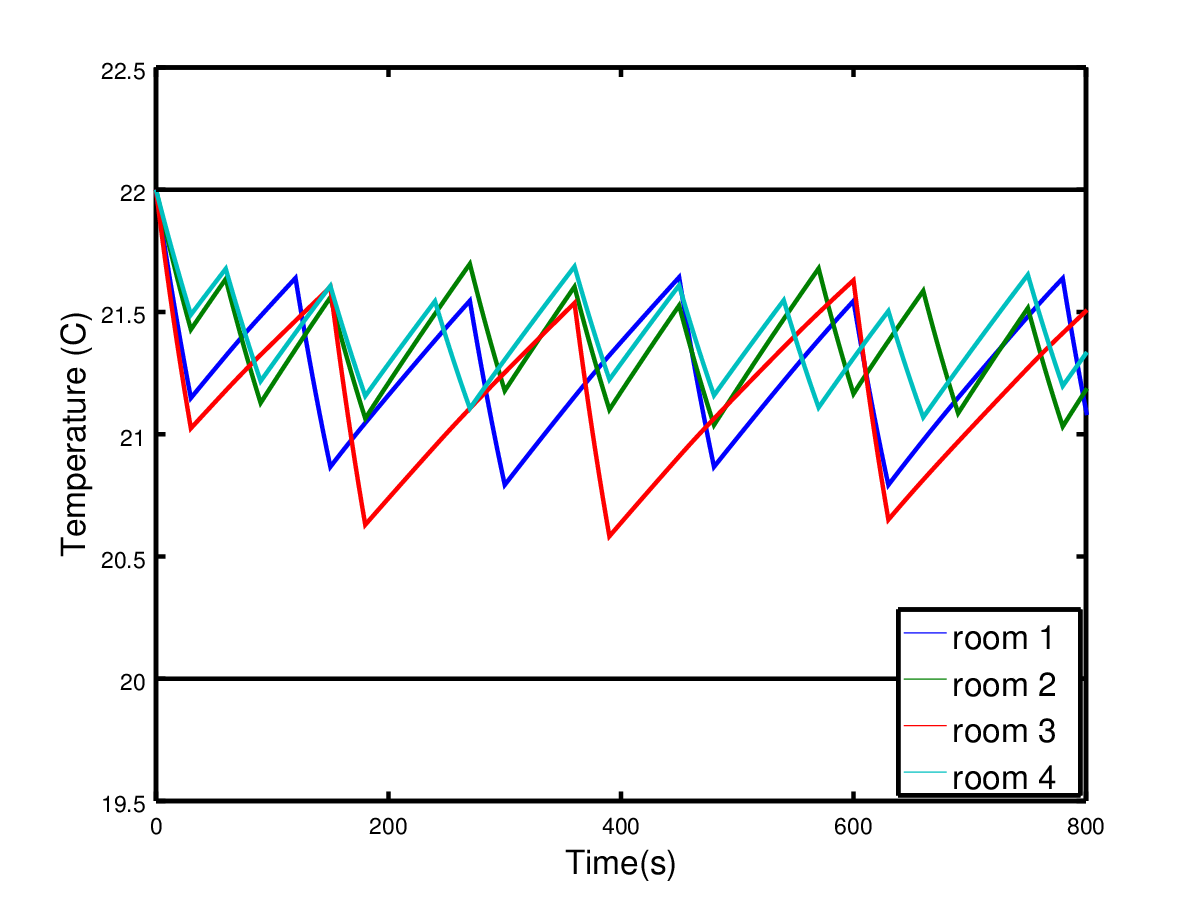
\includegraphics[scale=0.3]{simu_4rooms_central.png}%
% \caption{Simulation of the centralized controller from the initial condition $(22,22,22,22)$.}
%  \label{fig:NL_2}
%\end{figure}
%
%\begin{figure}[ht]
% \centering
%\hfill
 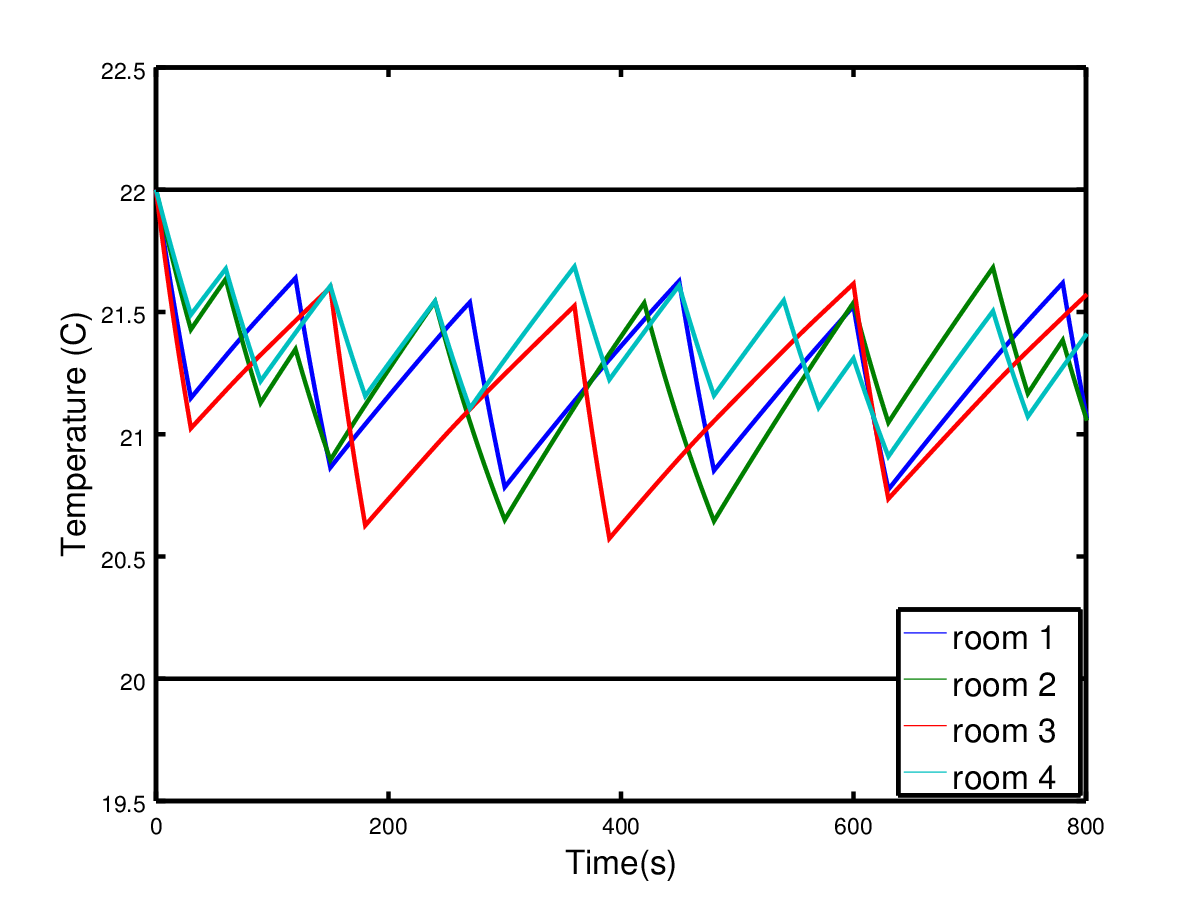
\includegraphics[scale=0.3]{simu_4rooms_compo.png}
 \caption{Simulation of the centralized (left) and distributed (right) controllers
 from the initial condition $(22,22,22,22)$.}
  \label{fig:simu_4rooms}
\end{figure}

 \section{Final remarks and future work}\label{sec:conc_part4}

 We have given a new distributed control synthesis method based on
 Euler's method.  The method makes use of the notions of
 $\delta$-ISS-stability and ISS Lyapunov functions.  From a certain
 point of view, this method is along the lines of
 \cite{dallal2015compositional} and \cite{kim2015compositional} which
 are inspired by small-gain theorems of control theory (see,
 \textit{e.g.}, \cite{jiang1994small}). In the future, we plan to
 apply our distributed Euler-based method to significant examples such
 as the 11-room example treated in
 \cite{larsen2015online,le2016distributed}.






% 
% \graphicspath{{part_2/figures}{part_2/figures/}}
% 
% \section{Introduction}
% %\subsection{Method of SNR'16 based on Runge-Kutta}
% As said in \cite{NL_minimator},
% in the methods of symbolic analysis and control of
% hybrid systems, the way of representing sets of state values
% and computing reachable sets for systems defined by
% ordinary differential equations (ODEs) is fundamental
% (see, e.g., \cite{Althoff2013a,girard2005reachability}).
% An interesting approach appeared recently, based on the
% propagation of reachable sets using guaranteed Runge-Kutta
% methods with adaptive step size control (see \cite{BMC12,immler2015verified}). In
% \cite{NL_minimator} such guaranteed
% integration methods are used in the framework of {\em sampled switched systems}.
% 
% %The approach n SNR'16 for validated
% %simulation is based on the numerical {\em Runge-Kutta} integration method method
% %[9], [10].
% Given an ODE of the form $\dot{x}(t)=f(t,x(t))$, and a {\em set} of initial values $X_0$,
% a symbolic (or ``set-valued'') integration method consists in computing a sequence of
% approximations $(t_n, \tilde{x}_n)$ of the solution $x(t; x_0)$ of the ODE
% with $x_0\in X_0$ such that $\tilde{x}_n \approx x(t_n; x_{n-1})$.
% Symbolic integration methods extend classical {\em numerical} integration methods which correspond to the case where $X_0$ is just a singleton $\{x_0\}$.
% The simplest numerical method is Euler's method in which $t_{n+1} = t_n + h$
% for some step-size $h$ and $\tilde{x}_{n+1} = \tilde{x}_n + h f(t_n,\tilde{x}_n)$; so
% the derivative of $x$ at time $t_n$, $f(t_n, x_n)$, is used as an
% approximation of the derivative on the whole time interval. This method is very simple
% and fast, but requires small step-sizes $h$.
% More advanced
% methods coming from the Runge-Kutta family use a few
% intermediate computations to improve the approximation
% of the derivative. The general form of an explicit $s$-stage
% Runge-Kutta formula
% of the form $\tilde{x}_{n+1}=\tilde{x}_n+h\Sigma_{i=1}^sb_ik_i$
% where $k_i=f(t_n+c_ih, \tilde{x}_n+h\Sigma_{j=1}^{i-1}a_{ij}k_j)$
% for $i=2,3,...,s$.
% A challenging question
% is then to compute a bound on the distance between
% the true solution and the numerical solution, i.e.:
% $\|x(t_n; x_{n-1}) - x_n\|$. This distance is associated to the {\em local
% truncation error} of the numerical method.
% In~\cite{NL_minimator}, 
% %(following the work of \cite{Nedialkov}),
% %[Berz and Makino01,Makino-Berz09,
% %Makino and Berz. Taylor models and other validated functional inclusion methods.
% %J. Pure and Applied Mathematics, vol. 4, no. 4, 2003.
% %Berz and Makino. Verified integration of ODEs and 
% %flows using differential algebraic
% %methods on high-order Taylor models. Reliable Computing, vol. 4, 1998.],
% such a bound is computed using the {\em Lagrange
% remainders} of Taylor expansions.
% This is achieved using {\em affine arithmetic} \cite{AffineA97}
% (by application of the Banach's fixpoint theorem and 
% Picard-Lindel\"of operator, see \cite{Nedialkov}). 
% In the end, the Runge-Kutta based method of \cite{NL_minimator} is an elaborated method
% that requires the use of affine arithmetic, 
% %the manipulation of vectors of intervals, 
% Picard iteration and 
% computation of Lagrange remainder.
% %\subsection{One-sided Lipschitz constant}
% 
% In contrast, in this paper, we use ordinary arithmetic
% (instead of affine arithmetic)
% and a basic Euler scheme (instead of Runge-Kutta schemes). We
% need neither estimate Lagrange remainders nor perform Picard iteration
% in combination with Taylor series.
% Our simple Euler-based approach is made possible  by having 
% recourse to the notion of {\em one-sided Lipschitz} (OSL) function
% \cite{Donchev98}.
% This allows us to bound directly the {\em global error},
% i.e. the distance between the approximate point~$\tilde{x}(t)$
% computed by the Euler scheme
% and the exact solution $x(t)$ for all $t\geq 0$
% (see Theorem~\ref{th:1}).
% 
% {\bf Plan.}
% In Section \ref{sec:rw}, we give  details on related work.
% In Section \ref{sec:OSL}, we state our main result that bounds
% the global error introduced by the Euler scheme in the context of systems
% with OSL flows.
% In Section~\ref{sec:appl}, we explain how to apply this result
% to the synthesis of symbolic control of sampled switched systems.
% We give numerical experiments and results
% in Section \ref{sec:experiment} for five exampes of the literature,
% and compare them with results obtained with the method of \cite{NL_minimator}.
% We give final remarks in Section \ref{sec:fr}.
% \section{Related work}\label{sec:rw}
% 
% Most of the recent work on the symbolic (or set-valued) integration of nonlinear ODEs is based
% on the upper bounding of the Lagrange remainders either in the framework of 
% Taylor series or Runge-Kutta schemes 
% \cite{Althoff2013a,BCD13,BMC12,CAS12,chen2013flow,NL_minimator,Makino2009,report,dit2016validated}.
% Sets of states are generally represented as vectors of intervals 
% (or ``rectangles'')
% and are manipulated  through interval arithmetic \cite{Moore66}
% or affine arithmetic \cite{AffineA97}.
% %
% Taylor expansions with Lagrange remainders are also used in the work
% of \cite{Althoff2013a}, which uses ``polynomial zonotopes'' 
% for representing sets of states in addition to interval vectors.
% %
% None of these works uses
% the Euler scheme nor the notion of one-sided Lipschitz constant.
% 
% In the literature on symbolic integration, the Euler scheme with OSL conditions
% is explored in \cite{Donchev98,Lempio95}.
% %
% Our approach is similar but establishes an {\em analytical} result for the global error of Euler's estimate
% (see Theorem \ref{th:1}) rather than analyzing, in terms of complexity,
% the speed of convergence to zero, the accuracy and the stability of Euler's method.
% 
% In the control literature, OSL conditions
% have been recently applied to control and stabilization 
% \cite{Abbaszadeh2010,Cai2015},
% but do not make use of Euler's method.
% %
% To our knowledge, our work applies for the first time Euler's scheme
% with OSL conditions to the symbolic
% control of hybrid systems.
% 
% \vspace{1em}
% {\bf Acknowledgement.}
% We are grateful to Antoine Girard, Jonathan Vacher, Julien Alexandre dit Sandretto and Alexandre Chapoutot for numerous helpful discussions.
% %
% This work has been partially supported by Federative Institute Farman (ENS Paris-Saclay and CNRS FR3311).
% 


% \end{document}
% EULER APPROXIMATION OF NONCONVEX DISCONTINUOUS DIFFERENTIAL INCLUSIONS Tzanko Donchev (2002)
% 
% The results are applied to numerical approximation of reachable sets of linar control problems by quadratic formulae and interpolation techniques for set-valued mappings. (...) the techniques apply to the set-valued mappingx of several variables as well, thus opening the access to finite element methods for the discrete approximation of nonliear differential inlusions in the, hopefully, near future.
% ???
% \footnote{Using the compactness of $R$, it is not difficult to show the following ``converse'' of Corollary \ref{propter:1}:
% 
% If there is a control $\sigma$ ensuring, for all $x\in R$, the properties
% of safety and recurrence w.r.t.  
% $\mathring{R}$ and~$\mathring{S}$, there exist $\delta>0$, points $x_1,...,x_m$,and patterns $\pi_1,...,\pi_m$
% such that conditions 1 and 2 of Corollary \ref{propter:1} hold.
% Following the construction of $\varepsilon$-bisimulation \cite{girard2010approximately}, we can also prove the existence of ``limit cycles'':
% 
% 
% \begin{proposition}
% Suppose the hypotheses and conditions 1 and 2 of Corollary \ref{propter:1} are satisfied. Then for any $x\in R$, there are $p$ pairwise distinct indices $i_1,...,i_p$ in $\{1,\dots,m\}$ such that:
% \begin{itemize}
% \item $\tilde{x}_{i_1}\in
% B(\tilde{\phi}_{\pi_{i_p}}(|\pi_{i_p}|\tau;\tilde{x}_{i_p}),\delta)$ and
% $\tilde{x}_{i_{k+1}}\in B(\tilde{\phi}_{\pi_{i_k}}(|\pi_{i_k}|\tau;\tilde{x}_{i_k}),\delta)$ for $k=1,\dots,p-1$, 
% \item $x\rightarrow_\sigma x_1^1$ and
% %\item 
% $x_1^1 \rightarrow_{\pi_{i_1}} x_2^1\rightarrow_{\pi_{i_2}} \cdots \rightarrow_{\pi_{i_{p-1}}}x_p^1\rightarrow_{\pi_{i_p}} x_1^2 \rightarrow_{\pi_{i_1}} x_2^2\rightarrow_{\pi_{i_2}} \cdots \rightarrow_{\pi_{i_{p-1}}}x_p^2\rightarrow_{\pi_{i_p}} x_1^3\rightarrow_{\pi_{i_1}} 
% %x_2^3\rightarrow_{\pi_{i_2}} 
% \cdots$
% \end{itemize}
% with $x^j_k \in B(\tilde{x}_{i_k},\varepsilon)$ for all $k=1,...,p$, all $j\geq 1$ and $\varepsilon=\frac{\delta}{1-e^{-\lambda\tau}}$.
% 
% 
% \end{proposition}}
% 
% Definition 2 (Abbaszadeh andMarquez [15]). The nonlinear 
% function $\Phi(x)$ is said to be {\em one-sided-Lipschitz} if there
% exists a constant
% $\lambda\in R$  such that 
% $$\langle \Phi(x_1)-\Phi(x2),x_1-x_2\rangle \leq \rho \| x_1-x_2\|^2$$ 
% where $\lambda$  is called the {\em one-sided Lipschitz constant}.
% 
% \subsection{Euler}
% Ernst Hairer and Christian Lubich:
% Numerical solution of
% ordinary differential equations.
% 
% 
% 
% The computational cost per step f implicit Euler method
% has increased dramatically: whereas the explicit
% Euler method requires a single function evaluation
% we now need to compute the Jacobian and
% then solve a linear system and evaluate f on each
% Newton iteration.
% 
% The problem
% is that the explicit Euler method and the differential
% equation have completely different stability
% behaviors unless the step size is chosen extremely
% small.
% 
% Such behavior is not restricted to the simple
% scalar example considered above, but extends to
% linear systems of differential equations in which
% the matrix has some eigenvalues with large negative
% real part, and to classes of nonlinear differential
% equations with a Jacobian matrix $\partial_y f$ having
% this property.
% 
% The explicit and implicit Euler
% methods also give rise to very different behaviors
% for nonlinear differential equations in which the
% function f(t, y) has a large (local) Lipschitz constant
% L with respect to y, while for some inner
% product the inequality
% $$\langle f(t, y) − f(t, z), y − z\rangle \leq \ell \| y − z\|$$
% holds for all t and y, z with a moderate constant
% $l << L$ (called a one-sided Lipschitz constant).
% \subsection{Local error}
% 
% For the explicit Euler method, the error after one
% step of the method starting from the exact solution,
% called the local error, is given as
% $$d_{n+1} = (y)t_n)+h(t_n,y_n)-y(t_n+h).$$
% By estimating the remainder term in the Taylor
% expansion of $y(t_n+h)$ at $t_n$, we can bound $d_{n+1}$ by
% $$\|d_{n+1}\|\leq Ch^2 \mbox{ with } C=\frac{1}{2}\max_{t_0\leq t\leq T}\|y''(t)\|,$$
% provided that the solution is twice continuously
% differentiable, which is the case if f is continuously
% differentiable.
% \subsection{Error propagation}
% the global error
% $e_n = y_n − y(t_n)$
% is the sum of the propagated local errors.
% With $M=(e^{(T-t_0)L}-1)C/L$, the global error satisfies
% $$\|e_n\|\leq Mh \mbox{ for } t_n\leq T.$$
% The numerical method thus converges to the exact
% solution as h tends to 0 with nh fixed, but only at
% first order, that is, with an error bound proportional
% to h.
% 
%  \subsection{Two-room building heater}
%  This example is taken from \cite{girard2012low}. It is a simple heating model 
%  of a two-room building. 
% %One of the rooms can be heated via a heating device. The two rooms 
% %% communicate such that heat from one room can diffuse to the other. Moreover, the rooms are surrounded
% % by an environment that has fixed temperature. By controlling when to turn 
% % the heating device on and off, we are interested in maintaining the two rooms at 
% % a comfortable temperature. 
% Let $T = (T_1 \ T_2)^\top$ be the state variable, where $T_i$ 
%  is the temperature of room $i$ ($i = 1,2$).
%  The dynamics of the system is given by the following equation:
%   $$
%  \dot{\left( \begin{matrix}T_1 \\ T_2 \end{matrix} \right)}=\left(\begin{matrix} - \alpha_{21} - \alpha_{e1}-\alpha_f{ u} & \alpha_{21} \\
%  \alpha_{12} &-\alpha_{12}-\alpha_{e2} \end{matrix}
% \right) 
% \left( \begin{matrix}T_1 \\ T_2 \end{matrix} \right) + \left( \begin{matrix}
%              \alpha_{e1} T_e + \alpha_f T_f { u} \\ \alpha_{e2}T_e
%             \end{matrix}\right).$$
%  where $u$ is a mode of value $0$ or $1$.
%   The values of the different parameters are the following: $\alpha_{12} = 5 \times 10^{-2}$,
%  $\alpha_{21} = 5 \times 10^{-2}$, $\alpha_{e1} = 5 \times 10^{-3}$, $\alpha_{e2} = 5 \times 10^{-3}$,
%  $\alpha_{f} = 8.3 \times 10^{-3}$, $T_e = 10$ and $T_f = 50$. 
%  
%     \begin{tabular}{|c|c|}
%    \hline 
%    $R$ & $[19,21]\times[19,21]$ \\
%    $S$ & $[18,22]\times[18,22]$ \\   
% \hline
%  Complete control & Yes \\
% \hline
% $\tau$ & 5 \\
% Time subsampling & $\tau/10$\\
% \hline
% $\lambda_1$  & -0.0041428              \\
% $\lambda_2$  &  -0.0080506\\
% $C_{1}$  &  -0.0033916                        \\
% $C_{2}$ & -0.0057549\\
% \hline
% Number of balls & 64 \\
% Pattern length & 2\\
% \hline
% CPU time &  0.5 seconds\\ \hline
%  \end{tabular}
%  
% %\bibliographystyle{plain}
% %\bibliography{minimator}
% %\end{document}          
% 
% \section{Numerical experiments and results}
% \label{sec:experiment}
% \subsection{4-room}
% This method has been implemented in the interpreted language Octave, and the experiments performed on a 2.80 GHz Intel Core i7-4810MQ CPU with 8 GB
% of memory.
% 
% We describe its application on a 4-room 16-switch building ventilation application adapted from
% \cite{meyer:tel-01232640}. The model has been simplified in order to get constant
% parameters.
% %, so that it can be handled by our linear tool MINIMATOR \cite{ulrich}, and
% %a comparison can be performed with the C++ implementation presented in \cite{le2016control}
% The system is a four room apartment
% subject to heat transfer between the rooms, with the external
% environment, with the underfloor, and with human beings.  The dynamics
% of the system is given by the following equation:
% \begin{equation*}
%  \frac{d T_i}{dt} = \sum_{j \in \mathcal{N}^\text{*} \setminus \{i\}} a_{ij} (T_j -
%  T_i) + \delta_{s_i} b_i (T_{s_i}^4 - T_i ^4 )  + c_i
%  \max\left(0,\frac{V_i - V_i^\text{*}}{\bar{ V_i} -
%    V_i^{\text{*}}}\right)(T_u - T_i), \quad \mbox{for } i=1,...,4.
% \end{equation*}
% 
% The state of the system is given by the temperatures in the rooms
% $T_i$, for $i \in \mathcal{N} = \{ 1 , \dots , 4 \}$.  Room~$i$ is
% subject to heat exchange with different entities stated by the indices
% $\mathcal{N}^\text{*} = \{1,2,3,4,u,o,c \}$.
% %
% We have $T_0=30, T_c=30, T_u=17$, $\delta_{s_i}=1$ for $i\in\mathcal{N}$.
% The parameters $T_{s_i}$, $V_i^\text{*}$, $\bar V_i$, $a_{ij}$, $b_i$,
% $c_i$ are given in \cite{meyer:tel-01232640} and have been identified
% with a proper identification procedure detailed in
% \cite{meyer2014ecc}. 
% %Note that we have neglected the term $\sum_{j
% %  \in \mathcal{N}} \delta_{d_{ij}}c_{i,j} \ast h(T_j - T_i)$ of
% %\cite{meyer:tel-01232640},
% %representing the perturbation induced by
% %the open or closed state of the doors between the rooms.\\
% %
% The control input is $V_i$ ($i \in \mathcal{N}$).
% %, is applied through the term
% %$c_i \max(0,\frac{V_i - V_i^\text{*}}{\bar{ V_i} -
% %  V_i^{\text{*}}})(T_u - T_i)$.  
% %A voltage $V_i$ is applied to force
% %ventilation from the underfloor to room $i$, and the command of an
% %underfloor fan is subject to a dry friction.  Because we work in a
% %switched control framework, $V_i$ can take only discrete values, which
% %removes the problem of dealing with a ``max'' function in interval
% %analysis. 
% In the experiment, $V_1$ and $V_4$ can take the values $0$V
% or $3.5$V, and $V_2$ and~$V_3$ can take the values $0$V or $3$V. This
% leads to a system of the form~\eqref{eq:sys_part2} with $\sigma(t) \in U =\{
% 1, \dots, 16 \}$, the $16$ switching modes corresponding to the
% different possible combinations of voltages $V_i$.  
% The sampling period is $\tau = 30$s.
% 
% 
% % Taking a
% %``max'' function into account with interval analysis is actually still
% %a difficult task. However, this term could have been taken into
% %account with a proper regularization (smoothing).
% 
% The recurrence set is $R = [20,22]^4$.
% The safety set is $S=[19.95,22.05]^4$, $T=[19.9,22.1]$.
% The computation of the constants $\lambda,L,C_j$ gives:
% $\lambda = 6.30 \times 10^{-3}$,
% $L = 1.01 \times 10^{-4}$,
% $C_j = 4.18 \times 10^{-6}$.
% We take $\delta=0.125\sqrt{2}$, which is greater than $\frac{C_j\tau}{\lambda}=0.0199$.
% %The maximal sampling time is $\tau_{max}=\frac{\lambda\delta}{C_j}=266.43$.
% We cover $R$ by  $m=8^4=4096$ balls of radius $\delta$, which are themselves contained in $S$.
% For each of these balls, our program finds a pattern (of length 1) that satisfies the conditions 1 and 2 of Corollary \ref{propter:1}.
% The whole computation takes $63$ seconds while the program of \cite{le2016control}
% takes $249$ seconds on the same example.
% %The synthesis is performed with a sampling time $\tau=30s$.
% %We compare on a simulation the results obtained by the control induced by these patterns with the contr described in \cite{le2016control}.
% %
% Compared simulations are given in Figure \ref{fig:simu}.
% 
% \begin{figure}[h]
% \centering
% \begin{tabular}{cc}
% % 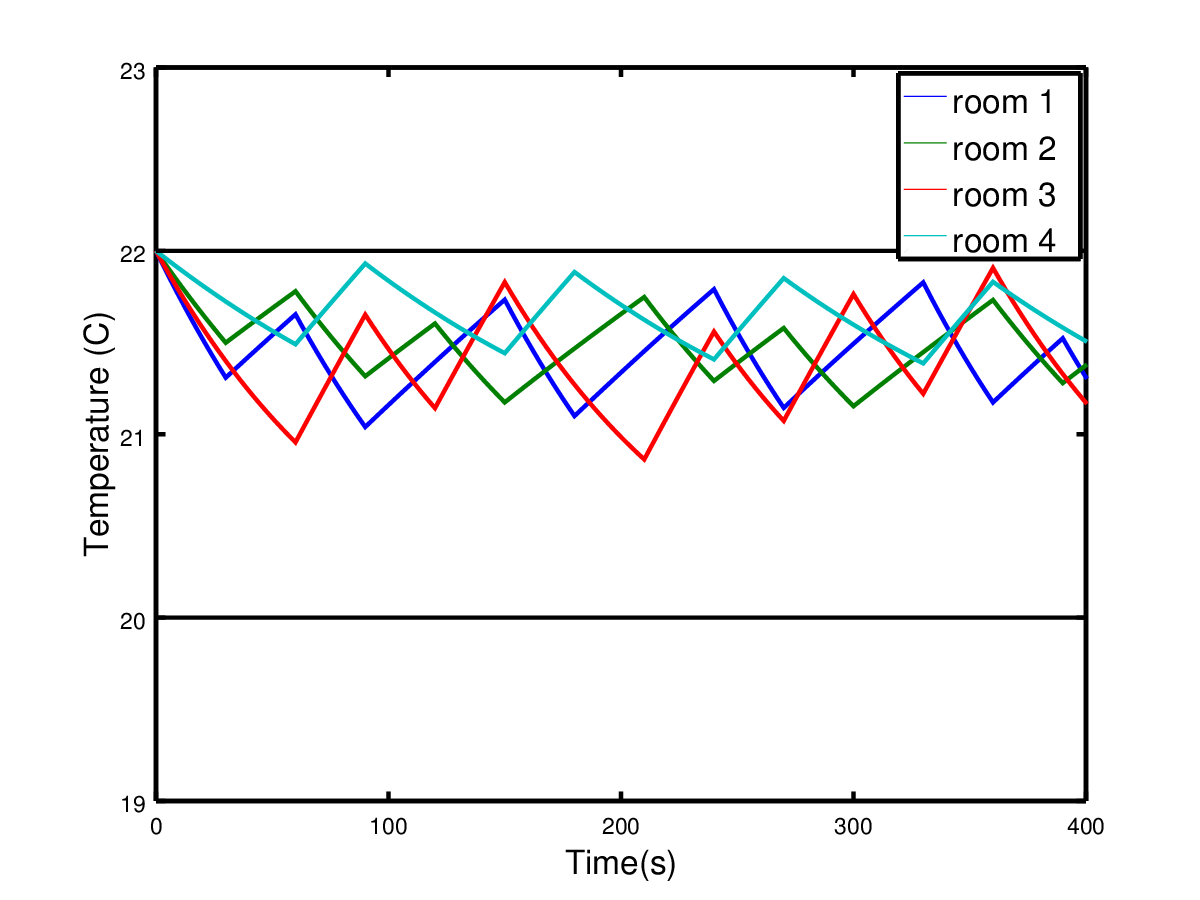
\includegraphics[width=0.45\linewidth,clip,trim=1cm 0cm 1cm 0cm]{simu4rooms3linear.png}
%  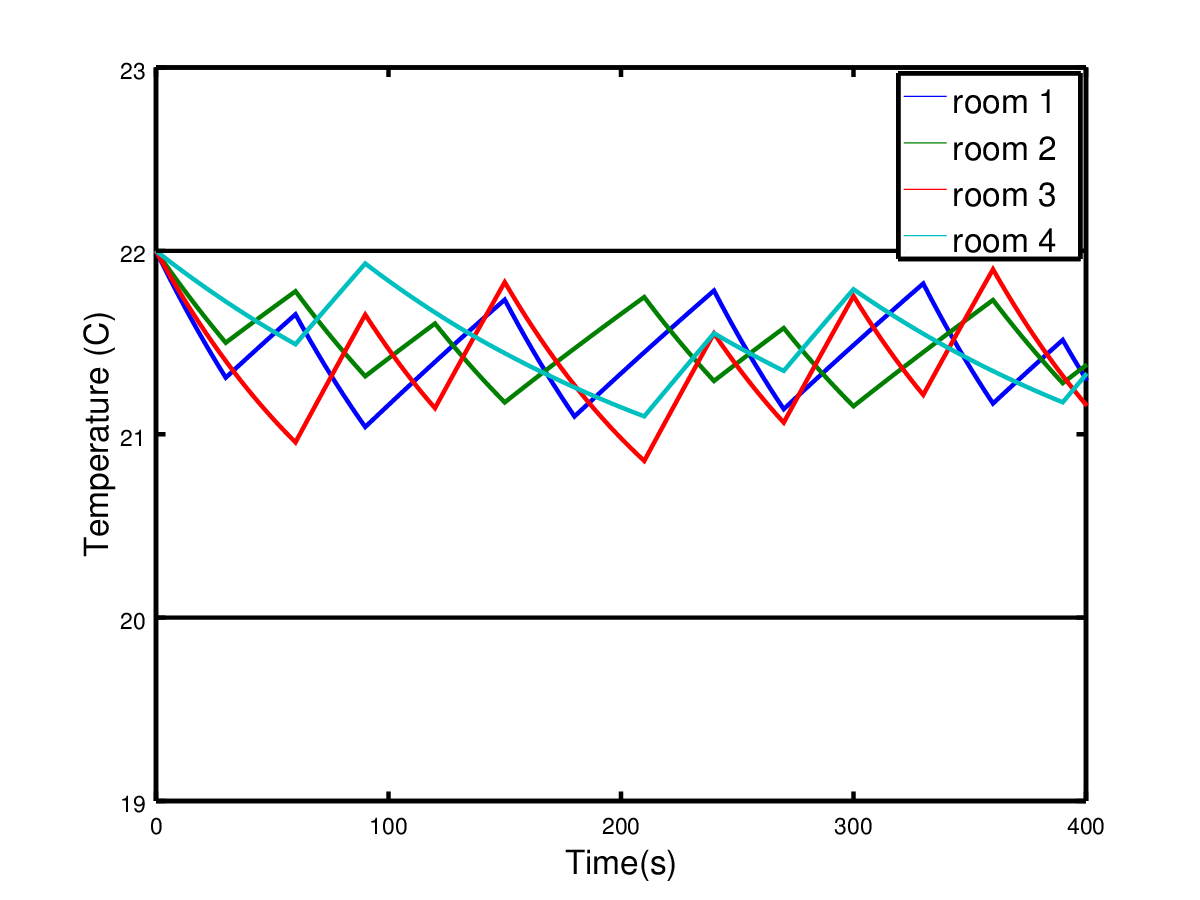
\includegraphics[width=0.4\linewidth,clip,trim=1cm 0cm 1cm 0cm]{figures/simu4roomslinearnew.png}
% &
%  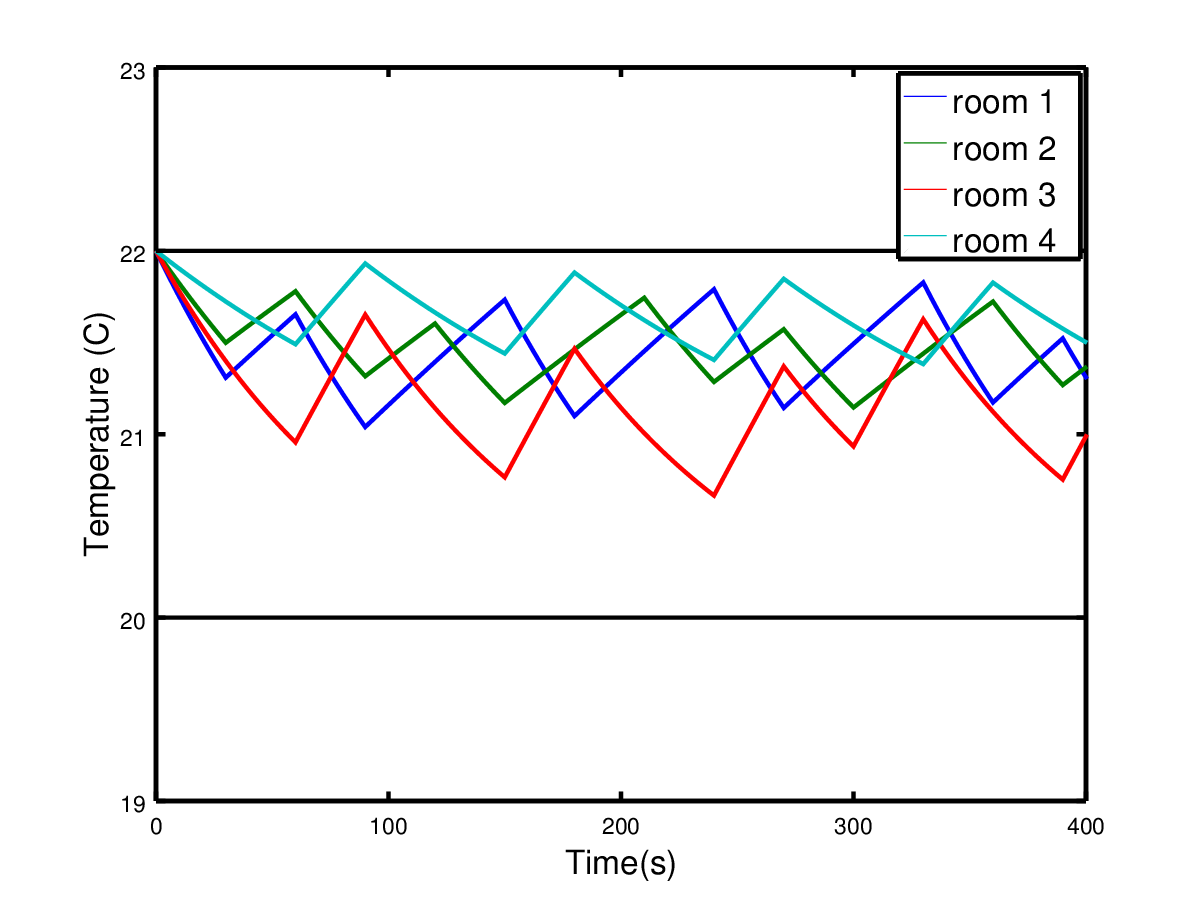
\includegraphics[width=0.4\linewidth,clip,trim=1cm 0cm 1cm 0cm]{simu4rooms2.png}
% \end{tabular}
% \label{fig:simu}
% \caption{Simulation of our synthesis method (left); simulation with the method of \cite{le2016control}  (right).}
% \end{figure}
% %\section{Numerical experiments}
%  
%  
%   \subsection{Polynomial example}
%  We consider the polynomial system taken from \cite{liu2013synthesis}:
% %
% \begin{equation}
%  \left \lbrack \begin{matrix}
%   \dot x_1 \\ \dot x_2
%  \end{matrix} \right \rbrack  =
%  \left \lbrack \begin{matrix} -x_2 - 1.5 x_1 - 0.5 x_1^3 + u_1 \\ x_1 + u_2 
%    \end{matrix} \right \rbrack.
% \end{equation}
% %
% The control inputs are given by $u = (u_1,u_2) =
% K_{\sigma(t)}(x_1,x_2)$, $\sigma(t) \in U = \{ 1,2,3,4 \}$, which correspond to
% four different state feedback controllers $K_1(x) = (0,-x_2^2 + 2)$,
% $K_2(x) = (0,-x_2)$, $K_3(x) = (2,10)$, $K_4(x) = (-1.5,10)$.  We thus
% have four switching modes. The disturbances are not taken into account.
% The objective is to visit infinitely often two zones $R_1$ and $R_2$,
% without going out of a safety zone $S$.
%  
%  \begin{tabular}{|c|c|}
%  \hline 
%  $R_1$ & $[-1,0.65]\times[0.75,1.75]$ \\
%  $R_2$ & $[-0.5,0.5]\times[-0.75,0.0]$ \\
%  $S$ &  $[-2.0,2.0]\times[-1.5,3.0]$ \\
%  \hline
%  Complete control & Yes \\
% \hline
% $\tau$ & 0.15 \\
% time subsampling & $\tau/20$\\
% \hline
% $\lambda_1$  & -1.5000e+00      \\
% $\lambda_2$  &  -1.0000e+00\\
% $\lambda_3$  &  -1.1992e-08  \\
% $\lambda_4$ &  -5.7336e-06 \\
% $C_{1}$  &  641.37         \\
% $C_{2}$ &  138.49\\
% $C_{3}$  &  204.50  \\
% $C_{4}$ & 198.64 \\
% \hline
% Number of balls & 16 \\
% Pattern length & 8\\
% \hline
% CPU time & 4203 \& 29 seconds \\ \hline
%  \end{tabular}
% 
%  \subsection{Two-tank system}
%  
%  The two-tank  system is a linear example taken from \cite{hiskens2001stability}. The system consists of two tanks and two valves.
% % The first valve adds to the inflow of tank 1 and the second valve is a drain valve for tank 2. 
% % There is also a constant outflow from tank 2 caused by a pump. The system is linearized at a desired
% % operating point. 
% The objective is to keep the water level in both tanks 
%  within limits using a discrete open/close switching strategy for the valves. 
%  let the water level of tanks 1 and 2 be given by $x_1$ and $x_2$ respectively. 
%  The behavior of $x_1$ is given by $\dot x_1 = -x_1 - 2$ when tank 1 valve is closed, 
%  and $\dot x_1 = -x_1 + 3$ when it is open. Likewise,
%  $x_2$ is driven by $\dot x_2 = x_1$ when tank 2 valve is closed and $\dot x_2 = x_1 - x_2 - 5$ when it 
%  is open. 
%  
%  
%  
%   \begin{tabular}{|c|c|}
% \hline
% $R$ & $[-1.5,2.5]\times[-0.5,1.5]$ \\
% $S$ & $[-3,3]\times[-3,3]$ \\
% \hline
%  Complete control & Yes \\
% \hline
% $\tau$ & 0.2 \\
% Time subsampling & $\tau/10$\\
% \hline
% $\lambda_1$  & 0.20711            \\
% $\lambda_2$  &  -0.50000\\
% $\lambda_3$  &  0.20711   \\
% $\lambda_4$ &  -0.50000  \\
% $C_{1}$  &  11.662                 \\
% $C_{2}$ & 28.917\\
% $C_{3}$  &  13.416 \\
% $C_{4}$ & 32.804 \\
% \hline
% Number of balls & 64 \\
% Pattern length & 6\\
% \hline
% CPU time & 52 seconds \\ \hline
%  \end{tabular}
%  
%  \subsection{Helicopter}
%  
%  The helicopter is a linear example
% taken from \cite{ding2011reachability}. The problem is to control a quadrotor helicopter toward 
%  a particular position on top of a stationary ground vehicle, while satisfying constraints 
%  on the relative velocity. 
% %By controlling the pitch and roll angles, we can modify the speed and the
% % position of the helicopter. A typical problem is 
% % to find a switching rule, depending on the position and velocity of 
% % the helicopter, in order to keep the system 
% % state within a safe area, avoiding excessive speed or distance in 
% % relation to the ground vehicle. 
% Let $g$ 
%  be the gravitational constant, $x$ (reps. $y$) the position 
%  according to $x$-axis (resp. $y$-axis), $\dot x$ (resp. $\dot y$) the velocity according to $x$-axis (resp. $y$-axis),
%  $\phi$ the pitch command and $\psi$ the roll command. 
%  The possible commands for the pitch and the roll are 
%  the following: $\phi,\psi \in \{ -10,0,10 \}$.
%  Since each mode correspond to a pair $(\phi,\psi)$, there are nine switched modes.
%  The dynamics of the system is given by the equation:
%  $$ \dot X = \begin{pmatrix}
%               0 & 1 & 0 & 0 \\ 
%               0 & 0 & 0 & 0 \\ 
%               0 & 0 & 0 & 1 \\               
%               0 & 0 & 0 & 0               
%               \end{pmatrix} X + \begin{pmatrix}
%               0 \\ g\sin(-\phi) \\ 0 \\ g\sin(\psi) \end{pmatrix}              
%  $$
% where $X = ( x \ \dot x \ y \ \dot y)^\top$. Since the variables $x$ and $y$
% are decoupled in the equations and follow the same equations (up to the sign of the command), it suffices
% to study the control for $x$ (the control for $y$ is the opposite).
% 
%    \begin{tabular}{|c|c|}
%    \hline 
%    $R$ & $[-0.3,0.3]\times[-0.5,0.5]$ \\
%    $S$ & (not applied???) $[-0.4,0.4]\times[-0.7,0.7]$ \\   
% \hline
%  Complete control & Yes \\
% \hline
% $\tau$ & 0.1 \\
% Time subsampling & $\tau/10$\\
% \hline
% $\lambda_1$  & 0.5            \\
% $\lambda_2$  &  0.5\\
% $\lambda_3$  &  0.5   \\
% $C_{1}$  &  1.77535                      \\
% $C_{2}$ & 0.5\\
% $C_{3}$  &   1.77535 \\
% \hline
% Number of balls & 256 \\
% Pattern length & 7\\
% \hline
% CPU time &  91 seconds\\ \hline
%  \end{tabular}
%  
%  
%  
% \subsection{DC-DC converter}
% 
% The DC-DC converter is a linear example taken from \cite{beccuti2005optimal}. 
% It was treated successfully with the state-space bisection method in a 
% discrete-time framework in \cite{fribourg2014finite}.
% %
% The system is a boost DC-DC converter with one switching cell.  There
% are two switching modes depending on the position of the switching
% cell. The dynamics is given by the equation $\dot x (t) =
% A_{\sigma(t)} x(t) + B_{\sigma(t)}$ with $\sigma(t) \in U = \{ 1,2
% \}$. The two modes are given by the matrices:
% 
% $$ A_1 = \left( \begin{matrix}
%           - \frac{r_l}{x_l} & 0 \\ 0 & - \frac{1}{x_c} \frac{1}{r_0 + r_c}
%          \end{matrix} \right)  \quad B_1 = \left( \begin{matrix}
%          \frac{v_s}{x_l} \\ 0 \end{matrix} \right) $$
% 
% 
% $$ A_2 = \left( \begin{matrix} - \frac{1}{x_l} (r_l +
%   \frac{r_0.r_c}{r_0 + r_c}) & - \frac{1}{x_l} \frac{r_0}{r_0 + r_c}
%   \\ \frac{1}{x_c}\frac{r_0}{r_0 + r_c} & - \frac{1}{x_c}
%   \frac{r_0}{r_0 + r_c}
%          \end{matrix} \right)  \quad B_2 = \left( \begin{matrix}
%          \frac{v_s}{x_l} \\ 0 \end{matrix} \right)  $$
% 
% with $x_c = 70$, $x_l = 3$, $r_c = 0.005$, $r_l = 0.05$, $r_0 = 1$,
% $v_s = 1$.  The sampling period is $\tau = 0.5$.  The parameters are
% exact and there is no perturbation.  We want the state to return
% infinitely often to the region~$R$, set here to $\lbrack 1.55 , 2.15
% \rbrack \times \lbrack 1.0 , 1.4 \rbrack$, while never going out of
% the safety set $S = \lbrack 1.54 , 2.16 \rbrack \times \lbrack 0.99 ,
% 1.41 \rbrack$.
% 
% 
% \begin{tabular}{|c|c|}
% \hline 
% $R$ & $[1.55,2.15]\times[1.0,1.4]$ \\
% $S$ & $[1.54,2.16]\times[0.99,1.41]$ \\
% \hline
%  Complete control & No \\
% \hline
% $\tau$ & 0.5 \\
% \hline
% $\lambda_1$  &  0.014215\\
% $\lambda_2$  & -0.142474\\
% $C_{1}$  & 6.7126e-05  \\
% $C_{2}$ &  2.6229e-02 \\
% 
% \hline
%  \end{tabular}
% 
% 
% 
% \section*{Appendix: Optimal time sampling for the lowest error bound}
% 
% >From Proposition \ref{prop:bound}, we have a bound of the deviation between
% the approximate and the exact system. This bound is\[
%   \gamma^2 =\delta^2 \exp(-\lambda \tau) + \frac{(C_j \tau)^2}{\lambda} (1 - \exp({-\lambda \tau}))
%  \].
%  
%  In fact, if we look at $\gamma$ as a function of $\tau$, there exists a $\tau$ minimizing this bound. In Figure \ref{fig:gamma}, we have represented 
%  $\gamma$ as a function of $\tau$ for the system described in Section \ref{sec:experiment}.
%  
%  \begin{figure}[h]
%   \centering
%   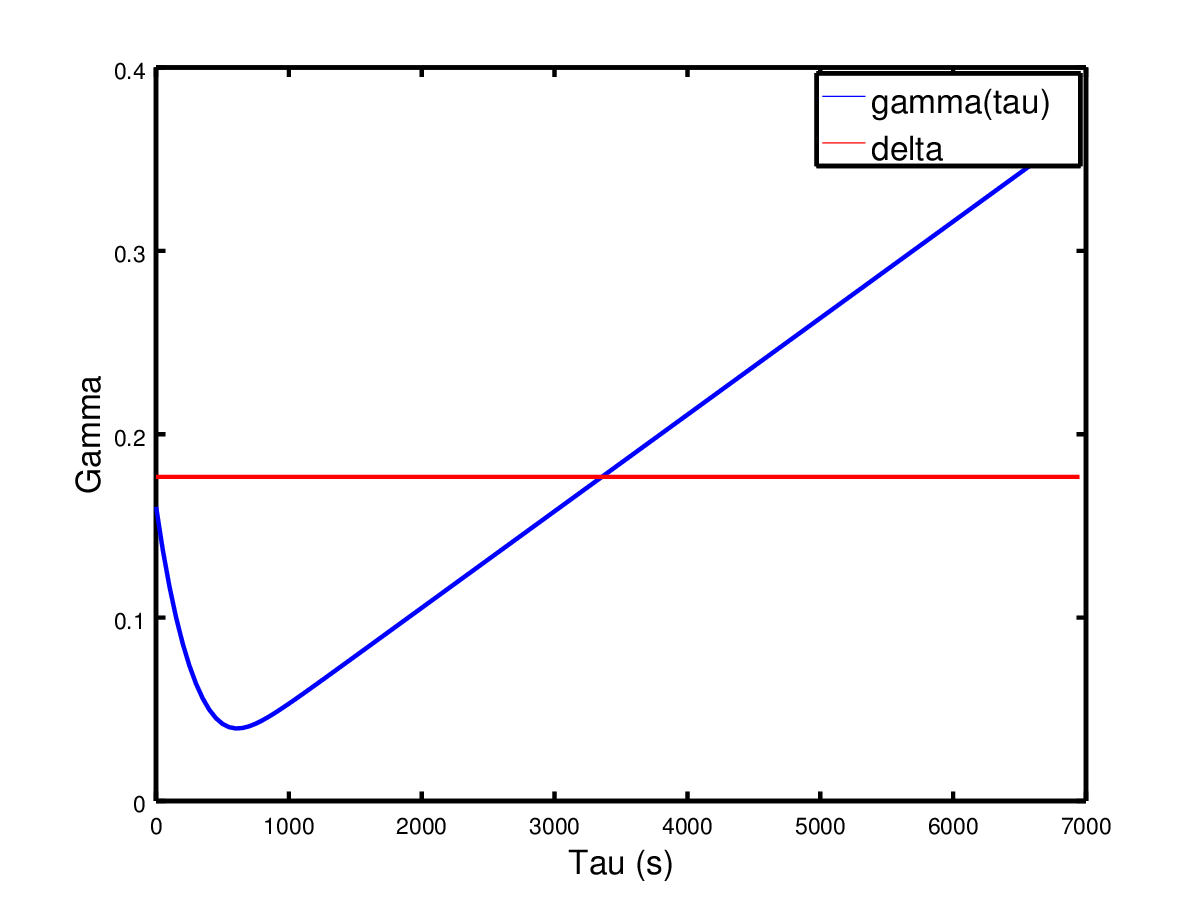
\includegraphics[width=0.55\linewidth]{gamma.png}
%   \caption{$\gamma$ as a function of $\tau$.}
%   \label{fig:gamma}
%  \end{figure}
% 
%  If no parameter $\tau$ is imposed by the system, then a good choice for 
%  the time sampling is the one minimizing $\gamma$, because it leads 
%  to a much easier synthesis (see Section \ref{sec:synthesis}).
%  
% 
% % \section{Appendix 1: Algorithms}
% % 
% % \centering
% % \fbox{
% % \begin{minipage}{0.82\textwidth}
% % \begin{algorithmic}
% % \STATE{\textbf{Function:} $Decomposition(W,R,S,B,D,R)$}
% %   \STATE{\begin{center}\line(1,0){150}\end{center}}
% % \STATE{\quad \textbf{Input:} A box $W$, a box $R$, a box $S$, a box $B$, a degree $D$ of bisection,
% % a length $R$ of input pattern}\STATE{\quad \textbf{Output:}$\langle\{(V_i,\pi_i)\}_{i},True\rangle$ or $\langle\_ ,False\rangle$}
% %   \STATE{\begin{center}\line(1,0){150}\end{center}}
% %   \STATE{ $(\pi,b) := Find\_Pattern(W,R,S,B,R)$}
% %   \IF{$b=True$}{
% %     \STATE{\textbf{return} $\langle\{(W,Pat)\},True\rangle$}
% %   }
% %   \ELSE
% %     \IF{$D = 0$} \RETURN{$\langle \_,False\rangle$} \ELSE
% %   \STATE{Divide equally $W$ into $(W_1,\dots, W_{2^{n}})$ \FOR{$i=1\dots2^{n}$}\STATE{\small{$(\Delta_i,b_i)$ := $Decomposition(W_i,R,S,B,D - 1,R)$}}\ENDFOR
% %   \RETURN $(\bigcup_{i=1\dots 2^{n}} \Delta_i,\bigwedge_{i=1\dots 2^{n}} b_i)$ } \ENDIF
% %  \ENDIF
% % \end{algorithmic}
% % \end{minipage}
% % }
% % 
% % \vspace{1em}
% % 
% % \fbox{
% % \begin{minipage}{0.82\textwidth}
% %  \begin{algorithmic}
% %  \STATE{\textbf{Function:} $Find\_Pattern(W,R,S,B,R)$}
% %    \STATE{\begin{center}\line(1,0){150}\end{center}}
% %  \STATE{\quad \textbf{Input:}A box $W$, a box $R$, a box $S$, a box $B$, a length $R$ of input pattern}
% %  \STATE{\quad \textbf{Output:}$\langle \pi,True\rangle$ or $\langle\_, False\rangle$}
% %    \STATE{\begin{center}\line(1,0){150}\end{center}}
% %    \FOR{$i=1\dots R$} \STATE{$\Pi :=$ set of input patterns of length $i$}
% %    \WHILE{$\Pi$ is non empty} \STATE{Select $\pi$ in $\Pi$}
% %    \STATE{$\Pi:= \Pi\setminus  \{\pi\}$}
% %    \IF{$Post_{\pi}(W) \subseteq R$ \AND $Tube_{\pi}(W) \subseteq S$ \AND $Tube_{\pi}(W) \bigcap B = \emptyset$ }{\RETURN{$\langle \pi,True\rangle$}} \ENDIF
% %    \ENDWHILE
% %    \ENDFOR
% %    \RETURN{$\langle \_,False \rangle$}
% % 
% %  \end{algorithmic}
% % \end{minipage}
% % }
% 
% 
% \section*{Superfluous material}
% We now extend the definitions of $\phi$ 
% % and $\tilde \phi$ 
% to sets of initial states.
% Let $Z_i$, $i \in I$ be a tile of $R$, we define:
% 
% \[ 
% \forall j \in U, \quad \phi(\tau;Z_i,j) = \{ \phi(\tau;x,j), x \in Z_i \}. 
% \]
% 
% % Likewise,
% % \[ 
% % \forall j \in U, \quad \tilde \phi_{\tilde x_0}(\tau;Z_i,j) = \{ \tilde \phi_{\tilde x_0}(\tau;x,j), x \in Z_i \}. 
% % \]
% 
% 
% 
% The principle of the algorithm is the following:
% for every tile $Z_i$, $i \in I$, look for a mode $j$ such that $\phi(\tau;Z_i,j) \subseteq R$.
% If every tile is controlled, then the algorithm succeeds. Otherwise, another (finer) tiling is tested.
% % Note that the algorithm can fail if some regions of $R$ are not controllable.
% 
% Because $\phi$ is hard to compute, we use the approximate model for the synthesis, {\em i.e.}
% using $\tilde \phi$. For every tile $Z_i$, $i \in I$, we denote the center of the tile by 
% $z_i$. Instead of computing $\phi(\tau;Z_i,j)$, 
% we compute $\tilde \phi_{z_i}(\tau;z_i,j)$, but the deviation error must be taken
% into account as follows.
% 
% Thanks to Proposition \ref{prop:bound}, we can bound the deviation
% between the approximate and the reduced model. 
% The tolerance $\delta$ is in fact the size of the half-diagonal of the tiles (see Figure \ref{fig:post} (a)).
% Indeed, if $x^0$ is in a tile $Z_i$, $\delta$ is the maximal distance 
% with the center of $Z_i$, and Proposition \ref{prop:bound} can be applied.
% If the approximate state~$z_i$ is sent in $R - {\gamma} = [x_1^{min} - \gamma ,x_1^{max} + \gamma]\times \dots \times [x_n^{min}-\gamma,x_n^{max}+ \gamma]$ (Figure \ref{fig:post} (a)), 
% the exact state will be sent in $R$ (Figure \ref{fig:post} (b)).
% It means that it is in fact sufficient to control the central point of a tile.
% This is formally stated in the theorem:
% 
% 
% \begin{theorem}
% Let $Z_i$, $i \in I$, be a tile of $R$, and let $\delta$ be the length of its
% half diagonal. If there exists a mode $j \in U$ such that
%  \[
%   \tilde \phi_{z_i}(\tau;z_i,j) \in R - {\gamma},
%  \]
% then we have
% \[
%  \phi(\tau;Z_i,j) \subseteq R.
% \]
% \end{theorem}
% 
% \begin{proof}
% Suppose there exists a mode $j \in U$ such that
% $ \tilde \phi_{z_i}(\tau;z_i,j) \subseteq R - {\gamma}$.
% 
% Let $x_0 \in Z_i$. We have $\| x_0 - z_i \| \leq \delta$
% 
% For any $\tilde x_0$ such that $\| x_0 - \tilde x_0 \| \leq \delta$, $\| \phi ( \tau;x_0,j) - \tilde \phi_{\tilde x_0}(\tau;\tilde x_0,j)  \|^2 \leq \gamma^2$.
% 
% In particular, $\| \phi ( \tau;x_0,j) - \tilde \phi_{z_i}(\tau;z_i,j)  \|^2 \leq \gamma^2$.
% 
% If the synthesis succeeds, we have $\phi_{z_i}(\tau;z_i,j) \in R - \gamma$, 
% and we can conclude that $\phi ( \tau;x_0,j) \in R$.
% %
% \end{proof}
% 
% Time sampling for non-increasing error
% \begin{corollary}
% Consider a point $\tilde{x}_0\in S$ such that $B(\tilde{\phi}_\sigma(t;\tilde{x}_0),\delta)\subseteq S$ for all $0\leq t\leq \tau$.\footnote{Since $\tilde{\phi}_\sigma$ is linear and $S$ is convex, it suffices to have
% $B(\tilde{\phi}_\sigma(t;\tilde{x}_0),\delta)\subseteq S$ for $t=0$ and $t=\tau$.}
% %for all $0\leq t\leq\tau$.
% %
% Suppose we are given a switched system \eqref{eq:sys_part2} satisfying (H0-H1)
% %and an approximate  model \eqref{eq:sys_part22} on $t\in [0,\tau)$
% with initial point $x_0\in B(\tilde{x}_0,\delta)$. 
% 
%  Suppose we are given a switched system \eqref{eq:sys_part2} 
% satisfying (H0-H1) with an initial point $x_0\in S$. Consider a point $\tilde{x}_0\in S$.
% %and an approximate  model \eqref{eq:sys_part22}. 
% Suppose: $\tau \leq \frac{\sqrt{\lambda} \delta}{ C_j}$.
% 
% If $x_0\in B(\tilde{x}_0,\delta)$ then, for all $0\leq t\leq \tau$, we have:
% %
% %$$\phi_j(t;x_0)\in B(\tilde{x}_0-t f_j(\tilde{x}_0), \delta).$$ 
% $$\phi_\sigma(t;x_0)\in B(\tilde{\phi}_\sigma(t;\tilde{x}_0), \delta).$$ 
% %
% \label{prop:1}
% \end{corollary}
% 
% %\begin{corollary}
% % Suppose we are given a switched system \eqref{eq:sys_part2} and an approximate 
% % model \eqref{eq:sys_part22}.
% %%Under hypotheses \ref{hyp:1} and \ref{hyp:2}, if $\|x_0 - \tilde x_0 \| \leq \delta$,
% %and if ,   we have, for all $j \in U$:
% %\[
% % \| \phi(\tau;x_0,j) - \tilde \phi_{\tilde x_0}(\tau;\tilde x_0,j) \| \leq {\delta}
% %\]
% %\end{corollary}
% \begin{proof}
% Suppose we want to have
% \[
% \|x(t)-\tilde x(t)\| \leq \|x_0-\tilde x_0\|.
% \]
% then a sufficient condition is
% \[
% \|x_0-\tilde x_0\|^2\, \exp(-\lambda t)
% + \frac{(C_j\, t)^2}{\lambda}\left( 1-\exp(-\lambda t) \right)
% \leq \|x_0-\tilde x_0\|^2.
% \]
% It yields 
% \[
% \frac{(C_j\, t)^2}{\lambda} \leq \|x_0-\tilde x_0\|^2.
% \]
% If we are given a tolerance $\|x_0-\tilde x_0\| \leq \delta$.
% We obtain
% \[
% t \leq \frac{\sqrt{\lambda} \delta}{C_j}.
% \]
% This leads to choosing a switching period inferior to this bound, for example
% %
% \begin{equation}
% \tau := \frac{\sqrt{\lambda} \delta}{2 C_j},
% \label{eq:dt}
% \end{equation}
% %
% in the Euler explicit scheme, in order to guarantee that the approximate solution
% goes near the exact solution.
% \end{proof}
% 
% \section{Introduction}
% In this paper, we present an application of symbolic (guaranteed) control synthesis method to a class
% of nonlinear switched systems. We show that under the hypothesis of strong monotony of the vector fields, an approximate 
% model based on a forward explicit Euler scheme can be used to build a guaranteed control.
% After implementation, we compare the method with \cite{le2016control} on the example
% of a four room apartment presented in \cite{meyer2014ecc}.
% 
% ``Robust infinity observer design for sampled-data Lipschitz nonlinear systems
% with exact and Euler approximate models''.
% Masoud Abbaszadeh, Horacio J. Marquez
% 
% Th2:asymptotical stabilty of the observer error dynamics
% 
% Th3: the algorithm
% proposed in Theorem 2 can be used to design an observer using
% Euler approximate discrete-time model (38) guaranteeing the
% observer practical convergence when applied to the (unknown)
% exact model (36). In other words, the estimates provided by the
% observer designed using Theorem 3 are practically convergent
% to the states of the (unknown) exact discrete-time model
% 
% In this paper, a new algorithm for robust $H_\infty$ nonlinear observer
% design for nonlinear discrete-time systems was proposed.
% The observer is robust in the sense that it can achieve convergence
% to the true state, despite nonlinear model uncertainty
% with optimized exogenous disturbance rejection ratio. When
% the exact discrete-time model of the system is not available,
% the same algorithm can still be used for the Euler approximate
% model.\\
% 
% 
% 
% 
% 
% The OSL condition we use is introduced in [8], [10] and naturally generalizes the
% existing notions of LC, of dissipativity (or monotonicity; cf., e.g., [2], [5]), and the
% (uniform) OSL condition [15], [7] of set-valued maps. It does not, however, imply continuity
% of $F(t, \cdot)$, as the Lipschitz condition, nor uniqueness of the trajectory starting
% from a given point, as the latter (uniform) OSL condition.
% Nevertheless, it assures stability of the attainable set, which is important for
% the sensitivity and approximations analysis of (1.1). This gives a positive answer
% to Artstein's question [1] of whether there is some general condition other than the
% Lipschitz one leading to stability of the attainable set.
% We give an implementation of the above-mentioned theorem to obtain error estimates
% for Euler discrete approximation of differential inclusions.\\
% 
% The one-sided Lipschitz condition generalizes the classical
% Lipschitz theory to a more general family of nonlinear systems
% [15]. It is worth mentioning that the one-sided Lipschitz constant
% can be zero or even negative while the Lipschitz constant must be
% positive. It is easy to see that any Lipschitz function is also 
% one-sided Lipschitz. However,the converse is not true. As it has been
% pointed out in [15,16], usually the one-sided Lipschitz constant can
% be found to be much smaller than the Lipschitz constant.\\
% 
